                                                                                                        %\pdfoutput=1
\documentclass[a4paper,11pt,twoside]{amsart}
\usepackage{amsmath}
\usepackage{geometry}
%\newproof{proof}{Proof}
\usepackage{amssymb, latexsym}
\usepackage{appendix}
\usepackage{verbatim}
%\usepackage{amscd}
\usepackage{enumerate}
\usepackage{comment}
\usepackage{txfonts}
\usepackage{float}
\usepackage{parskip}
\usepackage{lipsum}
\usepackage{hyperref}

%\usepackage{psfig}
\usepackage{graphicx}
%\usepackage{showkeys}  
%\usepackage{siunitx}
%\usepackage{tikz-cd}
%\usepackage{color}
%\usetikzlibrary{arrows}
% uncomment this when editing cross-references
%\numberwithin{equation}{section}
%\usepackage{hyperref}

%\volume{}
%\doi{}


% \usepackage{mathabx}


\usepackage{mathtools}%                  http://www.ctan.org/pkg/mathtools
\usepackage[tableposition=top]{caption}% http://www.ctan.org/pkg/caption
\usepackage{booktabs,dcolumn}%           http://www.ctan.org/pkg/dcolumn + http://www.ctan.org/pkg/booktabs
\usepackage[symbol]{footmisc}

\geometry{a4paper,total={6in,8in}, margin=1in}
\interfootnotelinepenalty=10000
     
%\theoremstyle{plain}

\newtheorem{theorem}{Theorem}[section]
%\newtheorem{theorem}[theorem]{Theorem}
\newtheorem{proposition}[theorem]{Proposition}
\newtheorem{hypothesis}[theorem]{Hypothesis}
\newtheorem{lemma}[theorem]{Lemma}
\newtheorem{corollary}[theorem]{Corollary}
\newtheorem{conjecture}[theorem]{Conjecture}
\newtheorem{principle}[theorem]{Principle}
\newtheorem{claim}[theorem]{Claim}

%\theoremstyle{definition}

%\newtheorem{roughdef}[subsection]{Rough Definition}
\newtheorem{definition}[theorem]{Definition}
\newtheorem{remark}[theorem]{Remark}
\newtheorem{remarks}[theorem]{Remarks}
\newtheorem{example}[theorem]{Example}
\newtheorem{examples}[theorem]{Examples}
%\newtheorem{problem}[subsection]{Problem}
%\newtheorem{question}[subsection]{Question}

\DeclareRobustCommand{\muS}{\text{\reflectbox{$\sum$}}}

\newcommand\F{\mathbb{F}}
\newcommand\E{\mathbb{E}}
\newcommand\R{\mathbb{R}}
\newcommand\Z{\mathbb{Z}}
\newcommand\N{\mathbb{N}}
\newcommand\D{\mathbb{D}}
\newcommand\C{\mathbb{C}}
\newcommand\Q{\mathbb{Q}}
\newcommand\T{\mathbb{T}}
\newcommand\e{\mathrm{e}}
\newcommand\sech{\mathrm{sech}}
\newcommand\KummerM{\mathrm{KummerM}}
\newcommand\LerchPhi{\mathrm{LerchPhi}}
\newcommand\erf{\mathrm{erf}}
\newcommand{\sgn}{\text{sgn}}
\renewcommand\Re{{\operatorname{Re\,}}}
\renewcommand\Im{{\operatorname{Im\,}}}
\renewcommand{\thefootnote}{\fnsymbol{footnote}}
\newcommand\Log{{\operatorname{Log}}}
\newcommand\eps{\varepsilon}

\renewcommand\P{\mathbf{P}}

% include the ifthen package for conditional compilation
\usepackage{ifthen}

% comment out the next command for the release version
%\newcommand{\debugmode}{}

\ifthenelse{\isundefined{\debugmode}}{
%%%%%%%%%%%%%%%%%%%%%%%%%%%%%%%%%%%%
%%% code to include for shipping %%%
%%%%%%%%%%%%%%%%%%%%%%%%%%%%%%%%%%%%
\newcommand{\unfinished}{\hl{\textnormal{***UNFINISHED***}}}
\newcommand{\addthis}{\hl{\textnormal{***ADD THIS***}}}
\newcommand{\selfnote}[1]{\todo{\textnormal{#1}}\xspace}
%
\newcommand{\verifiedeq}{=}
\newcommand{\unverifiedeq}{=}
\newcommand{\defeq}{=}
\newcommand{\verifiedleq}{\leq}
\newcommand{\unverifiedleq}{\leq}
\newcommand{\verifiedgeq}{\geq}
\newcommand{\unverifiedgeq}{\geq}
\newcommand{\verifiedlessthan}{<}
\newcommand{\unverifiedlessthan}{<}
\newcommand{\verifiedgreaterthan}{>}
\newcommand{\unverifiedgreaterthan}{>}
\newcommand{\missingcitation}{\cite{?}\xspace}
%%%%%%%%%%%%%%%%%%%%%%%%%%%%%%%%%%%%
%%%%%%%%%%%%%%%%%%%%%%%%%%%%%%%%%%%%
%%%%%%%%%%%%%%%%%%%%%%%%%%%%%%%%%%%%
}{
%%%%%%%%%%%%%%%%%%%%%%%%%%%%%%%%%%%%
%%% code to include for debugging %%
%%%%%%%%%%%%%%%%%%%%%%%%%%%%%%%%%%%%
\newcommand{\unfinished}{\hl{\textnormal{***UNFINISHED***}}}
\newcommand{\addthis}{\hl{\textnormal{***ADD THIS***}}}
\newcommand{\selfnote}[1]{\todo{\textnormal{#1}}\xspace}
%
\newcounter{eqverifcounter}
\setcounter{eqverifcounter}{1}

\newcommand{\verifiedeq}{\stackrel{\checkmark}{=}}
\newcommand{\unverifiedeq}{\stackrel{{\color{red!70!black}\scriptscriptstyle \arabic{eqverifcounter}}}{=}\stepcounter{eqverifcounter}}
%
\newcommand{\defeq}{\stackrel{\scriptscriptstyle \textnormal{def}}{=}}
%
\newcommand{\verifiedleq}{\stackrel{\checkmark}{\le}}
\newcommand{\unverifiedleq}{\stackrel{{\color{red!70!black}\scriptscriptstyle \arabic{eqverifcounter}}}{\le}\stepcounter{eqverifcounter}}
%
\newcommand{\verifiedgeq}{\stackrel{\checkmark}{\ge}}
\newcommand{\unverifiedgeq}{\stackrel{{\color{red!70!black}\scriptscriptstyle \arabic{eqverifcounter}}}{\ge}\stepcounter{eqverifcounter}}
%
\newcommand{\verifiedlessthan}{\stackrel{\checkmark}{<}}
\newcommand{\unverifiedlessthan}{\stackrel{{\color{red!70!black}\scriptscriptstyle \arabic{eqverifcounter}}}{<}\stepcounter{eqverifcounter}}
%
\newcommand{\verifiedgreaterthan}{\stackrel{\checkmark}{>}}
\newcommand{\unverifiedgreaterthan}{\stackrel{{\color{red!70!black}\scriptscriptstyle \arabic{eqverifcounter}}}{<}\stepcounter{eqverifcounter}}
%
\newcommand{\missingcitation}{[{\color{red!70!black}{$\textrm{\bf ?}_{\scriptscriptstyle\arabic{eqverifcounter}}$}}]\stepcounter{eqverifcounter}\xspace}
%%%%%%%%%%%%%%%%%%%%%%%%%%%%%%%%%%%%
%%%%%%%%%%%%%%%%%%%%%%%%%%%%%%%%%%%%
%%%%%%%%%%%%%%%%%%%%%%%%%%%%%%%%%%%%
}
%%%%%%%%%%%%%%%%%%%%%%%%%%%%%%%%

\setlength\evensidemargin\oddsidemargin
%\setlength{\parindent}{0cm}

\usepackage{color}
\definecolor{almond}{rgb}{0.94,0.87,0.8}

\let\oldv\verbatim
\let\oldendv\endverbatim

\def\verbatim{\par\setbox0\vbox\bgroup\oldv}
\def\endverbatim{\oldendv\egroup\fboxsep0pt \noindent\colorbox[gray]{0.8}{\usebox0}\par}

\title[Visualising the flows of orthogonal polynomial expansions of the Riemann $\Xi$-function]{Visualising the flows of orthogonal polynomial expansions \\ of the Riemann $\Xi$- function}

\author{Dolph Dwars, Kalpesh Muchhal}
\date{\today, v3.3}
\address{\tt{{\it E-mail Address}: ra.dwars@quicknet.nl}}
\address{\tt{{\it E-mail Address}: kalpesh.muchhal@iitbombay.org}}

%%% AMS subject classification
\subjclass[2010]{Primary 33C45, 11M06}
% 33-XX Special functions
% 33Cxx      Hypergeometric functions
% 33C45      Orthogonal polynomials and functions of
%            hypergeometric type (Jacobi, Laguerre, 
%            Hermite, Askey scheme, etc.)
%
% 11-XX Number theory
% 11Mxx	     Zeta and $L$-functions: analytic theory
%   11M06    $\zeta (s)$ and $L(s, \chi)$

\keywords{Orthogonal polynomials, Riemann xi function, Riemann zeta function, Riemann hypothesis, De Bruijn-Newman constant}

\begin{document}

\begin{abstract}
In a comprehensive paper \cite{rom}, Dan Romik derives new infinite series expansions for the Riemann $\Xi(t)$ function in three specific families of orthogonal polynomials; the Hermite polynomials, the symmetric Meixner-Pollaczek polynomials and the continuous Hahn polynomials. He also launched the idea to use the Poisson kernel from the theory of orthogonal polynomials to distort the Riemann $\Xi-$function and thereby induce a 'flow' in its zeros that obeys some dynamical evolution law. Building on Romik's work, we initially aimed at visualising only his three flows, however ended up embarking on a broader journey that included the six continuous polynomials families in the Askey scheme. For each of them we visualised their flows and derived their governing laws. We observe that the visualised flows can be categorised into two types. As a by-product, we derived simpler expressions for the expansion coefficients of the Laguerre, Meixner Pollaczek, Continuous Hahn, Continuous Dual Hahn and Wilson flows.  
\end{abstract}

\maketitle

\section{Introduction and preliminaries}

When a conjecture about the zeros of function is hard to proof, a line of attack could be to use suitable approximations of this function that are easier to handle. Another approach is to distort the function by a smartly chosen parameter and to study the evolution of its zeros. These approaches have also been used to attack the Riemann Hypothesis (RH). Early last century, Pólya started work in this direction and spurred the development of many new ideas (see chapters 1 of \cite{rom} and \cite{pol} for a comprehensive historic overview). This culminated in the 2018 Polymath15 project \cite{pol} that managed to successfully reduce the range of validity of the RH (measured by the De Bruijn-Newman constant) when distorting the Riemann $\Xi-$function by a special parameter. It also demonstrated how through further numerical verification of the RH, this range would be reduced further. Both authors of the current paper have been involved on the numerical/computational side of the project and the production of data and associated graphs. 

Shortly after the Polymath15 project had completed in 2019, Dan Romik published a paper in which he proposed an interesting new line of attack \cite{rom}. He started from the work of Turán who explored the more 'natural' idea of expanding the Riemann $\Xi-$function into a series involving orthogonal Hermite polynomials. Romik built on this idea and managed to derive new infinite series expansions for the Riemann $\Xi$-function, including rigorous asymptotics for their coefficients, in three specific families of orthogonal polynomials; the Hermite polynomials, the symmetric Meixner-Pollaczek polynomials and the Continuous Hahn polynomials. He also introduced the provoking idea of using an intrinsic property from the theory of orthogonal polynomials, the so-called 'Poisson kernel', to distort $\Xi$ and thereby induce a 'Poisson flow' of its real and complex zeros that obey some dynamical evolution law. To quote Romik p19, chapter 2 of \cite{rom}: 

\begin{quotation}
 \textit{...the point is that Poisson flows are a method of approximation that allows us considerable freedom in choosing a system of orthogonal polynomials to use, and it is conceivable that this might lead to new families of approximations with useful properties.} 
\end{quotation}

Inspired by Romik's work, we started from the idea to use the computational learnings from the Polymath15 project and make an attempt to visualise the newly developed Poisson flows. Initially we followed his approach to directly link a generating function of a family of orthogonal polynomials (for a specific choice of parameters) to the kernel of the Fourier cosine integral of the Rieman $\Xi-$function. This leads to significantly simpler expansion coefficients and paves the way for a rigorous proof of convergence and asymptotics. However, we found that this approach seems only viable for a relatively small set of families and parameters. All families of orthogonal polynomials have been organised in the so-called Askey scheme. In this hierarchy, they are ranked by increasing hypergeometric complexity and the number of free parameters. Since each family has its own characteristics and we wanted to produce the flows for each of them, we decided to compute the generic Fourier series expansion that is independent of the function to be expanded. This has the following advantages: 
\begin{itemize}
\item The Poisson flows as well as their governing laws can be derived and visualised for all continuous families in the Askey-scheme (the discrete/finite families are not suitable for our purpose, since they only allow expansions at integer values. We also excluded the $q-analogues$).
\item We can easily adjust our code by just plugging in any other sufficiently fast decaying entire function other than $\Xi$. For comparative purposes we chose to include the flows of the $\Xi_i$ function (explained later in this paper) that shares a couple equivalent properties. 
\end{itemize}
However, it also comes with disadvantages:
\begin{itemize}
\item The computationally intense $\Xi$-function will show up in each coefficient, although a key insight from the Polymath15 project (p16, remark 4.1 of \cite{pol}) is that evaluating $\Xi$ at smaller heights has become quite tractable when using modern software and hardware.
\item A clear disadvantage of our generic expansion approach is that it doesn't open up an easy path towards establishing the asymptotics of the coefficients, nor does it pave the way for a rigorous proof of convergence in $\mathbb{C}$. This paper will therefore be more of an experimental kind. Having said that, during our investigations we have developed a significant amount of "by-products" that expand on Romik's initial work on the three families of orthogonal polynomials. We managed for instance to generalise his Meixner-Pollaczek and Continuous Hahn expansions towards a broader set of parameters than $\frac34$. We also found similar expansions (i.e. with easy to compute coefficients) for the Laguerre, Continuous Dual Hahn and Wilson polynomial families. For readability purposes, we shared these results and their derivations in the appendix.  
\end{itemize}

We will focus our work on visualising the evolution of the real zeros only. Pairs of complex zeros typically occur when two trajectories of real zeros 'collide' at a certain point in 'time'. We have developed the tools to visualise the complex zeros (requiring a 3D-plot), but leave these out of scope for now. 

For our computations we require all relevant formulae  associated with a specific family of orthogonal polynomials (hypergeometric function, weight, orthogonality relation, leading coefficients, etc.) and for this we will follow the 2010 standard reference by Koekoek, Lesky and Swarttouw \cite{koe} that has been complemented by Koornwinder's 2022 paper containing new insights, additions and errata \cite{koesup}. The literature about orthogonal polynomials comes with its own historically evolved nomenclature that we will obviously strictly follow. However, some labels of the polynomials are not unique and for the unique labelling of the Poisson flows, we allowed ourselves a bit more freedom to ensure unambiguous and easy reference for the reader. We don't use any special mathematical symbols, but the Pochhammer symbol $(x)_n$ will appear quite often in the paper and reflects the rising factorial.

\section{Structure of the paper}
In the next chapters we will numerically and visually explore the Poisson flows of the real zeros of infinite series expansions for $\Xi(t)$ and $\Xi_i(t)$ into six families of orthogonal polynomials. We start with an introduction of the Askey-scheme in chapter \ref{askeyscheme} followed by the derivations of the Poisson flow in chapter \ref{poissonflow} and the laws that govern the flows in chapter \ref{lawspoissonflow}. Chapter \ref{functobexpanded} introduces our target functions $\Xi$ and $\Xi_i$ and shows their Pólya-De Bruijn flows. After some computational and mathematical considerations in chapters \ref{mathcons} and \ref{compcons}, we will explain how the computational results were verified in chapter \ref{checks}. We will end the paper by presenting our results in chapter \ref{results} and a concluding remark in chapter \ref{concremarks}. We have moved the many "by-products" of our investigations as well as their derivations to appendix \ref{specexpansions}. 

\pagebreak
\section{Askey scheme}\label{askeyscheme}

The Askey scheme is a way of organizing orthogonal polynomials into a hierarchy (see \cite{koe}).
\begin{figure}[H]
  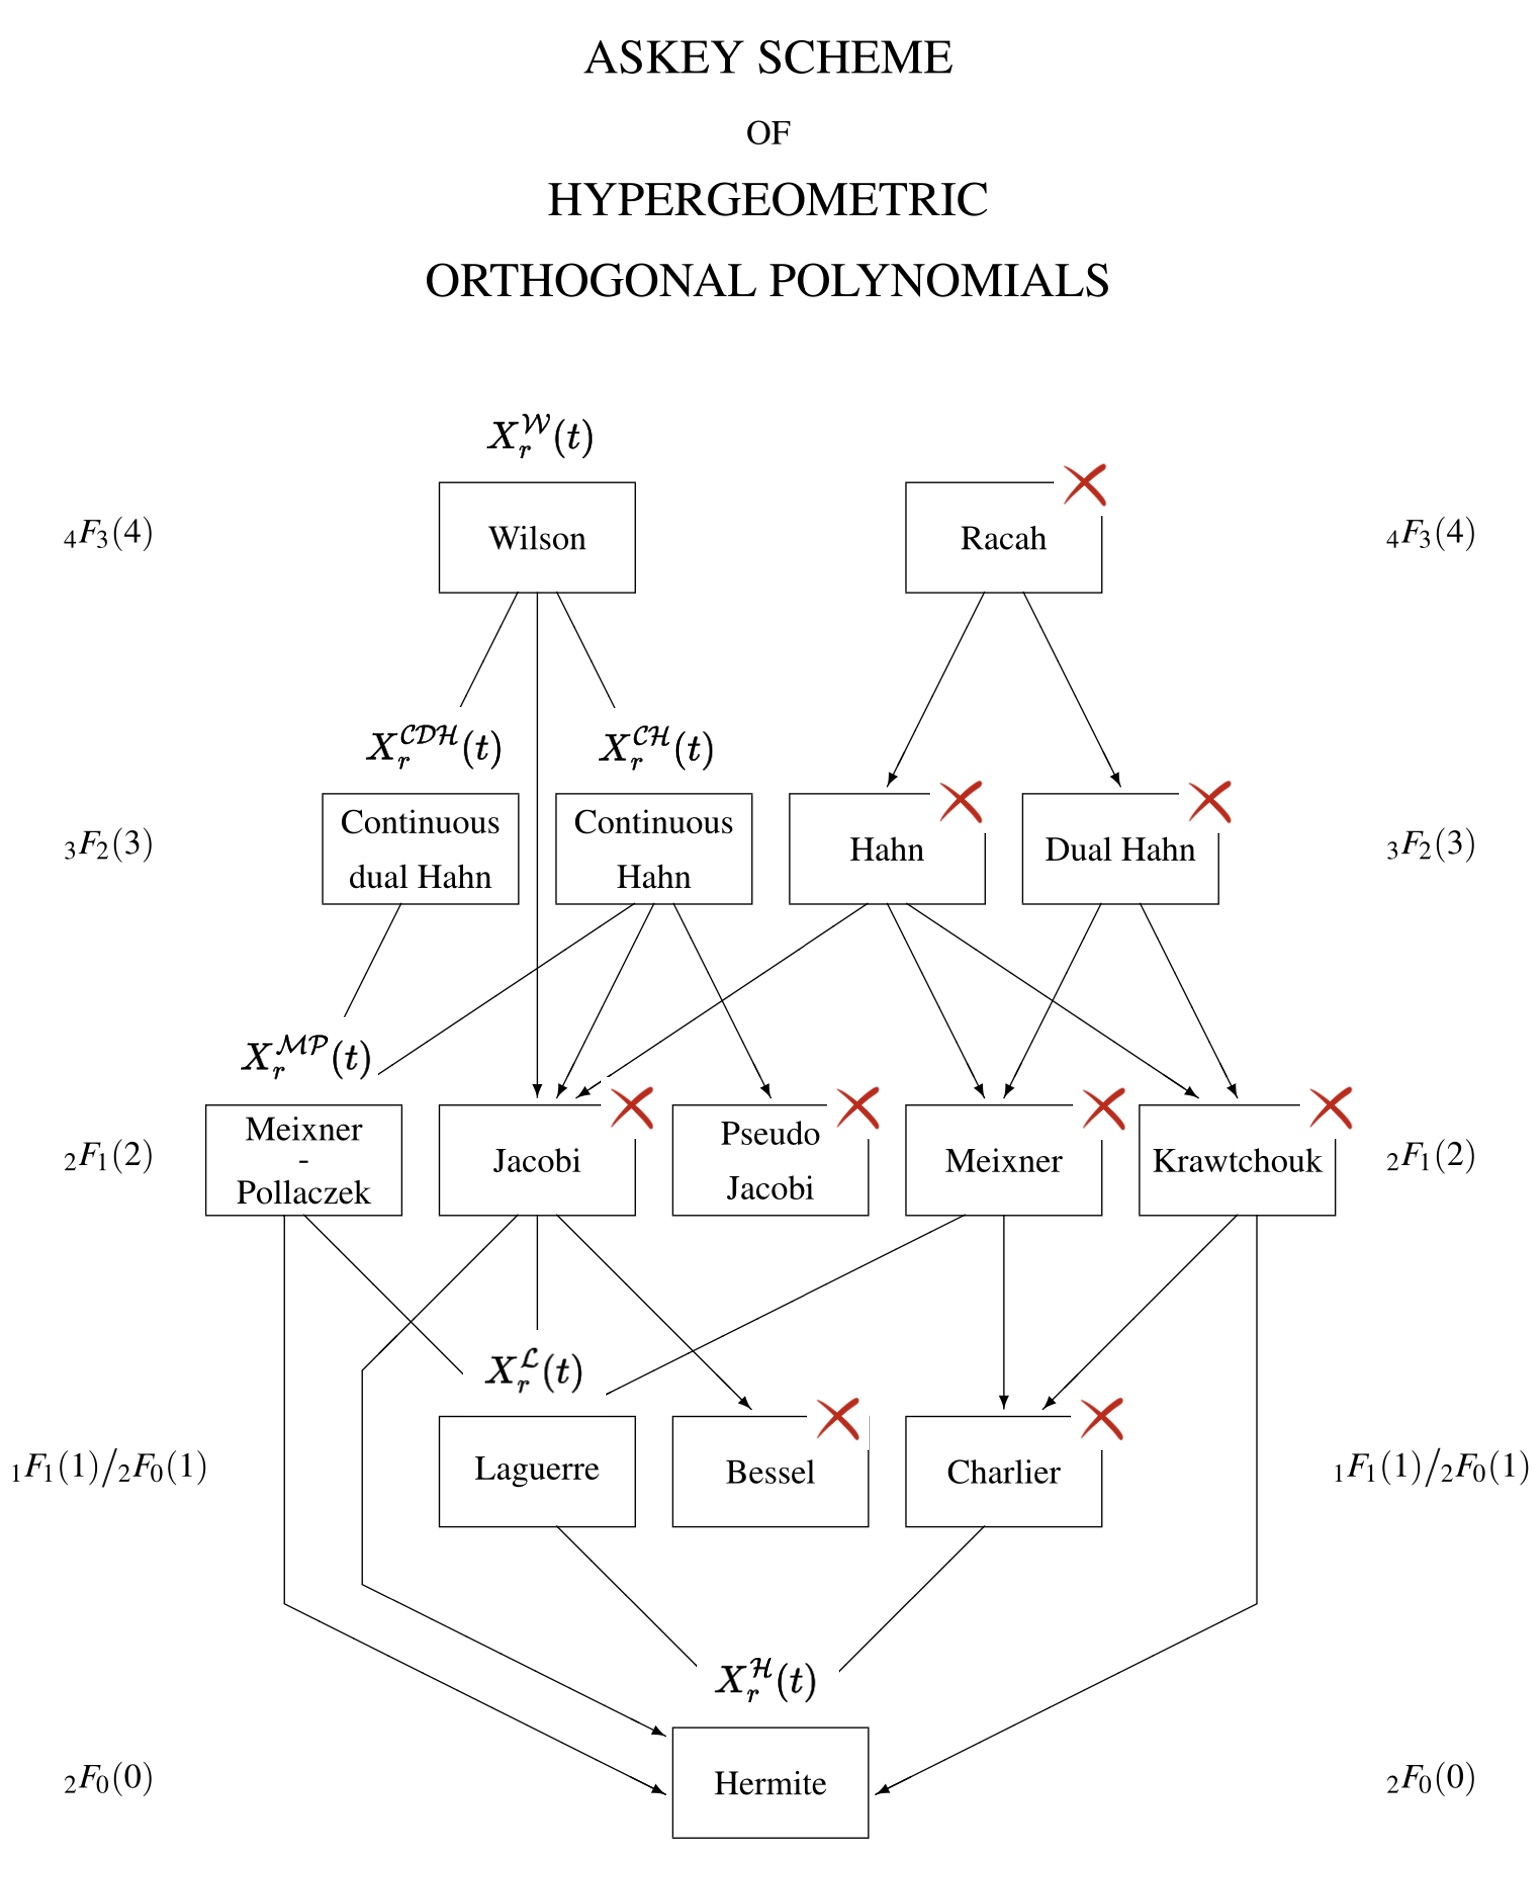
\includegraphics[width=0.8\linewidth]{Askeyschemenew.jpeg}
  \caption{Askey scheme of orthogonal polynomials. The complexity of the polynomials increases from bottom to top which is reflected in the assocated hypergeometric function. The number between parenthesis reflects the number of free parameters. The arrows always flow from top to bottom and denote possible transformations (mostly based on infinite limits) from one family into another. We have added the labels $X_r^{\mathcal{\Phi}}(t)$ as an easy and unique reference to the Poisson flow connected to a polynomial family. The discrete families have been 'crossed out' from our scope. The polynomials in each family in the Askey scheme are eigenfunctions of either a second order differential operator or a second order difference operator with eigenvalue $n\kappa_n$, where $\kappa_n$ equals either $1$ or equals $n$ plus a term depending on the parameters. In fact, for the families not crossed out in Figure \ref{fig:askey}, only Continuous Hahn and Wilson have $\kappa_n$ non-trivial.}
  \label{fig:askey}
\end{figure}

\pagebreak
\section{The Poisson flow} \label{poissonflow}
In paragraph 2.5 of \cite{rom}, Romik introduces the interesting concept of a "Poisson flow". This is based on the idea that any series expansion of the Riemann $\Xi$-function in a system of orthogonal polynomials comes equipped with its own flow based on the standard construction of the so-called Poisson kernel from the theory of orthogonal polynomials. 

We start by denoting $\phi \verifiedeq \left(\phi_n\right)_{n=0}^\infty$ as the family of polynomials that are orthogonal with respect the weight function $w_x$. We have the orthogonality relation:

\begin{equation}\label{ortrel}
 \int_{\mathbb{R}} \phi_n(x)\,\phi_m(x)\,w_x\, \mathrm{d}x = M_n\,\delta_{m,n}
\end{equation}

where $\delta_{m.n}$ is the Kronecker delta function. The quantity $M_n$ is the closed form of the orthogonality relation where the two indices are equal. The Poisson flow for function $F$ is now defined as follows:

\begin{equation}\label{poiflow}
X^\phi_z(t)\defeq
    \begin{cases}
        \int_{-\infty}^{\infty} p_z(t, \tau)\,F(\tau)\,w(\tau)\,\mathrm{d}\tau & \text{if } 0 < z < 1\\
        \\
        F(t) & \text{if } z = 1
    \end{cases}
\end{equation}

where $F(t)$ is the function to be expanded and $p_z(t, \tau)$ is the Poisson Kernel defined as:

\begin{equation}\label{poiker}
 p^\phi_z(x,y) \defeq \sum_{n=0}^\infty\frac{z^n}{M_n}\, \phi_n(x)\,\phi_n(y)
\end{equation}

with $M_n \verifiedeq \int_\mathbb{R}\phi_n(x)^2\,w_x\,\mathrm{d}x$. Note that depending on the polynomial family, the integral could also be an infinite sum.

\textit{Remark:} For some families of orthogonal polynomials, the Poisson Kernel $p_z(t, \tau)$ itself can be expressed into a hypergeometric form. In the literature these are referred to as expressions for "bilinear sums" or "bilinear generating functions" (see for instance \cite{genoverview} and \cite{meipolgen}). We derived a few of these simplified expressions, and one of them has been used for our computations (see \ref{lagpoiclosed}).

Swapping the summation and integration in the Poisson flow (assuming Fubini's theorem applies for $F(t)$), recovers the underlying Fourier series expansion into a family of orthogonal polynomials $\phi$:
\begin{align}
 X^\phi_z(t) &\verifiedeq \sum_{n=0}^\infty z^n\,\gamma_n\,\phi_n(t) \\
 \gamma_n &\verifiedeq \frac{1}{M_n}\,\int_{-\infty}^\infty F(x)\,\phi_n(x)\,w_x \,\mathrm{d}x
\end{align}

It is this generic structure that we decided to use for our computations, since it allows for the once-off calculation of the coefficients $\gamma_n$ for a certain set of chosen parameters for the orthogonal polynomial under study. All six orthogonal polynomials in scope can now be expressed into a hypergeometric function and a leading factor $g_n$ that is only dependent on $n$ and the free parameters. This allows us to optimise the coefficient pre-computations a bit further:

\begin{align}
 X^\phi_z(t) &\verifiedeq \sum_{n=0}^\infty z^n\,\gamma_n\,g_n\,{}_pF_q(n,t,\text{parms})\\
 \gamma_n &\verifiedeq  \frac{1}{M_n}\,\int_{-\infty}^\infty F(x)\, g_n\,{}_pF_q(n,x, \text{parms})\,w(x) \,\mathrm{d}x
\end{align} 

Collecting all terms that are independent of $r$ and $t$, we will pre-compute $\gamma_n$ as follows:
\begin{align}
 X^\phi_z(t) &\verifiedeq \sum_{n=0}^\infty z^n\,\gamma_n\,{}_pF_q(n,t, \text{parms}) \label{defflow} \\
 \gamma_n &\verifiedeq  f_n\,\int_{-\infty}^\infty F(x)\,{}_pF_q(n,x,\text{parms})\,w(x) \,\mathrm{d}x \qquad \text{with } f_n = \dfrac{g_n^2}{M_n} \label{deffn}
\end{align} 

In view of our treatment of the Poisson Flow in section 5 we substiture in (\ref{defflow}):
\begin{equation}
 z \defeq \exp(-\kappa_n\,r), \quad r > 0
\end{equation}

Accordingly we rewrite (\ref{defflow}) as:
\begin{equation}
 X^\phi_r(t) \verifiedeq \sum_{n=0}^\infty \exp(-n\kappa_n\,r)\,\gamma_n\,{}_pF_q(n,t, \text{parms}) \label{defflow1}
\end{equation}

\section{The laws that govern the evolution of the zeros under the Poisson Flow} \label{lawspoissonflow}
When varying parameter $r$ in the Poisson Flow (\ref{defflow1}) between $0$ and $\infty$, the real and or complex zeros of function $F$ at time $r=0$ will start to move. Subsequent changes in $r$ will therefore induce a 'trajectory' of zeros. Trajectories of real zeros can 'collide' (not cross) neighbouring trajectories and transform  into a conjugated pair of complex zeros. An interesting property is 'hyperbolicity', that forces trajectories of zeros, once real, to stay real 'forever' (this can occur moving forwards or backwards in "time" $r$). In this section we aim to derive the laws that govern the flow of zeros expressed into the first derivative of time of a zero at a certain point in time. 

We have actually started visualising the flow (\ref{defflow}) with $z$, however found that using the exponential variable $r$ in \ref{defflow1}) induces more 'natural' flows (i.e. resembling the collision patterns of the Pólya-De Bruijn flows). It therefore seems that this mapped distortion factor provides a more 'natural' way to describe the flow and it also directly paves the way for deriving the governing laws.    

We will now demonstrate how this works for the Generalised even Laguerre (using its Partial Differential Equation - PDE) and the Wilson (using its Differential Difference Equation - DDE) orthogonal polynomial families. The derivation of all the other families follows exactly the same lines and the results have been captured in appendix \ref{eqsused}.

\subsection{Evolution of the zeros under the Generalised Laguerre Poisson Flow governed by a PDE} \label{Laguerrelawspoissonflow}
We start from the Generalised Laguerre Poisson Flow (\ref{lagflow}):
\begin{align}
  M(r,t)=  X^{\mathcal{L}}_r(t;a)\left[F(t)\right] &\verifiedeq \sum_{n=0}^\infty \gamma_n(a)\,{}_1F_1\left(-n, a+1,t\right)\,\exp(-nr)\quad r \ge 0
\end{align} 

For brevity, we also set $H_n(t) \defeq {}_1F_1\left(-n, a+1,t\right)$. 

\begin{lemma}\label{proofBes1} The function $M(r,t)$ satisfies the Partial Differential Equation (PDE): 
\begin{align}
 \frac{\partial}{\partial r}M(r,t) \verifiedeq \frac12\,\frac{\partial^2}{\partial t^2}M(r,t) + \left(\frac{\alpha+\frac12}{x}-x\right)\,\frac{\partial }{\partial t}M(r,t)
\end{align}
\end{lemma}

\begin{proof}
Using (\ref{lagPDE}) we obtain:
\begin{align}
 \frac{\partial}{\partial r}M(r,t) &\verifiedeq  \frac{\partial}{\partial r}\,\left(\sum_{n=0}^\infty \gamma_n(a)\,H_n(t)\,\exp(-2nr)\right) \\
 &\verifiedeq 2\,\sum_{n=0}^\infty \gamma_n(a)\,H_n(t)\,\left(-n\right)\,\exp(-2nr) \\
 &\verifiedeq 2\,\sum_{n=0}^\infty \gamma_n(a)\,\left(\frac14\,\frac{\partial^2}{\partial t^2}H_n(t)+ \left(\frac{2\alpha+1}{4\,x}-\frac{x}{2}\right)\, \frac{\partial}{\partial t}H_n(t)  \right)\, \exp(-nr)\\
 &\verifiedeq \frac12\,\frac{\partial^2}{\partial t^2}M(r,t) + \left(\frac{\alpha+\frac12}{x}-x\right)\,\frac{\partial }{\partial t}M(r,t)
\end{align}
\end{proof}

Now let $z_k(r)$ be the $k$-th simple zero of the flow $M(r,t)$ for a some fixed parameter $a$.
 
\begin{lemma}\label{proofBes2} The evolution of the zeros under the flow $M(r,t)$ is governed by the following equation:
\begin{align}
 \frac{\mathrm{d}}{\mathrm{d} r}z_k(r) \verifiedeq -\,\sum_{j \ne k}^{'} \frac{1}{z_k(r)-z_j(r)} -\frac{\alpha+\frac12}{z_k(r)}+z_k(r)
\end{align}
\end{lemma}
where $j \in \mathbb{Z}\backslash\{0\}, j \ne k$. The prime indicates $j$ and $-j$ terms should be summed together (the remaining $k=-j$ term is summed separately).
\begin{proof}

We start from the observation that:
\begin{align}
M(r,z_k(r)) &\verifiedeq 0 \\
\frac{\mathrm{d}}{\mathrm{d} r} \big(M(r,z_k(r))\big) &\verifiedeq 0 \\
\frac{\partial M}{\partial r}(r,z_k(r))+ \frac{\partial M}{\partial t}(r,z_k(r))\,\frac{\mathrm{d} z_k(r)}{\mathrm{d} r} &\verifiedeq 0 \\
-\frac12\,\frac{\partial^2}{\partial z_k(r)^2}M(r,z_k(r)) -\left(\frac{\alpha+\frac12}{x}-x\right)\,\frac{\partial }{\partial t}M(r,z_k(r))  &\verifiedeq \frac{\partial}{\partial t}M(r,z_k(r))\,\frac{\mathrm{d}}{\mathrm{d} r}z_k(r)
\end{align}

Since we assumed $z_k(r)$ to be simple, its derivative with respect to $t$ can't be zero, hence we can rewrite this as follows:

\begin{align}
\frac{\mathrm{d} }{\mathrm{d} r}z_k(r) &\verifiedeq \dfrac{-\frac12\,\frac{\partial^2}{\partial t^2}M(r,z_k(r)) -\left(\frac{\alpha+\frac12}{z_k(r)}-z_k(r)\right)\,\frac{\partial }{\partial t}M(r,z_k(r))}{ \frac{\partial}{\partial t}M(r,z_k(r))} \\
&\verifiedeq -\frac12\,\dfrac{\frac{\partial^2}{\partial t^2}M(r,z_k(r))}{ \frac{\partial}{\partial t}M(r,z_k(r))}  -\left(\frac{\alpha+\frac12}{z_k(r)}-z_k(r)\right) \label{secondder}
\end{align}

From Taylor expansion of $M(r,z_k(r)), \frac{\partial}{\partial t}M(r,z_k(r))$ and $\frac{\partial^2}{\partial t^2}M(r,z_k(r))$ around the simple zero $z_k$ we get:

\begin{align}\label{taylor}
 \dfrac{\frac{\partial^2}{\partial t^2}M(r,z_k(r))}{\frac{\partial}{\partial t}M(r,z_k(r))} \verifiedeq 2\,\lim_{z\to z_k} \left(\dfrac{\frac{\partial}{\partial t}M(r,z)}{M(r,z)} -\frac{1}{z - z_k(r)} \right)
\end{align}

\pagebreak
We also have the Hadamard product: 

\begin{align}
  M(r,z) \verifiedeq M(r,0)\prod_j^{'}\left(1-\frac{z}{z_j}\right)
\end{align}

where the prime indicates that the $j$ and $-j$ factors are multiplied together. We now take its logarithmic derivative:

\begin{align}
  \dfrac{\frac{\partial}{\partial t}M(r,z)}{M(r,z)} \verifiedeq \sum_j^{'} \frac{1}{z-z_j}
\end{align}

Plugging this into (\ref{taylor}) and then into (\ref{secondder}) gives the result.
\end{proof}

\subsection{Evolution of the zeros under the Wilson Poisson Flow governed by a DDE} \label{Wilsonlawspoissonflow}

We start from the Wilson Poisson Flow (\ref{wilflow}) and let $\kappa_n = n+a+b+c+d-1$: 

\begin{align}
  M(r,t) \verifiedeq X^\mathcal{W}_{r}(t;a,b,c,d) &= \sum_{n=0}^\infty \gamma_n(a,b,c,d)\,H_n(t)\,\exp(-n\,\kappa_n\,r)
\end{align} 

For brevity we have set $H_n(t) \defeq {}_4F_3\left(\left[-n, \kappa_n,a+it, a- it\right], \left[a+b, a+c, a+d\right], 1\right)$.
\begin{lemma}\label{proofWil1} The function $M(r,t) \verifiedeq X^\mathcal{W}_{r}(t;a,b,c,d)$ satisfies the Differential Difference Equation: 
\begin{align}
 \frac{\partial}{\partial r}M(r,t) \verifiedeq -B(t)\,M(r,t+i) +\left(B(t)+D(t)\right)M(r,t)- D(t)\,M(r,t-i) \label{WilDDE}
\end{align}

 with $B(t) \verifiedeq \dfrac{(a-it)\,(b-it)\,(c-it)\,(d-it)}{2it(2it-1)}$ and $D(t)=\dfrac{(a+it)\,(b+it)\,(c+it)\,(d+it)}{2it(2it+1)}$.
\end{lemma}

\begin{proof}
Using (\ref{wildde}) we obtain:

\begin{align} 
 \frac{\partial}{\partial r}M(r,t) &\verifiedeq  \frac{\partial}{\partial r}\,\left(\sum_{n=0}^\infty \gamma_n(a)\,H_n(t)\,\exp(-n\,\kappa_n\,r)\right) \\
 &\verifiedeq \sum_{n=0}^\infty \gamma_n\,H_n(t)\,\left(-n\,\kappa_n\right)\,\exp(-n\,\kappa_n\,r) \\
 &\verifiedeq \sum_{n=0}^\infty \gamma_n\,\bigg(-B(t)\,H_n(t+i) +\left(B(t)+D(t)\right)H_n(t)- D(t)\,H_n(t-i)\bigg)\,\exp(-n\,\kappa_n\,r)  \\
 &\verifiedeq-B(t)\,M(r,t+i) +\left(B(t)+D(t)\right)M(r,t)- D(t)\,M(r,t-i)
\end{align}
\end{proof}

\pagebreak
Now let $z_k(r)$ be the $k$-th simple zero of the flow $M(r,t)$ for a some fixed set of parameters $a,b,c,d$.
\begin{lemma}\label{proofWil2} The evolution of the zeros under the Wilson Poisson flow for a finite version of $M(r,t)$, named $M_p(r,t)$, is governed by the following equation:

\begin{align}
 \frac{\mathrm{d}}{\mathrm{d} r}z_k(r) \verifiedeq i\,B(z_k(r))\, \prod^{'}_{\substack{1\le j \le n \\j \ne k}}\left(1+ \frac{i}{z_k(r)-z_j(r)}\right) -i\,D(z_k(r))\,\prod^{'}_{\substack{1\le j \le n \\j \ne k}} \left(1-\frac{i}{z_k(r)-z_j(r)}\right)
\end{align}

where $j \in \mathbb{Z}\backslash\{0\}, j \ne k$. The prime indicates $j$ and $-j$ terms should be multiplied together (the remaining $k=-j$ term is multiplied separately). The finite entire function $M_p(r,t)$ is:

\begin{align}
M_p(r,t) \verifiedeq \sum_{k=0}^n \gamma_k \, H_k(t)\,\exp(-k\,\kappa_k\,r) 
\end{align}

and defined as a solution to the DDE (\ref{WilDDE}), where $p(t) \defeq \prod_{k=1}^n(t-z_k)$ and the initial condition $M_p(0,t) \defeq p(t)$. Note that $p(t)$ is a monic polynomial of degree $n$ with simple zeros for $t$ in a neighbourhood of $t_0$ where the polynomial $r \mapsto M_p(t,r)$ has simple zeros. Remark: formally we can let $n\to\infty$ and make it approach $M(r,t)$ infinity close.
\end{lemma}

\begin{proof}
We start from the observation that:

\begin{align}
M_p(r,z_k(r)) &\verifiedeq 0 \\
\frac{\mathrm{d}}{\mathrm{d} r} \big(M_p(r,z_k(r))\big) &\verifiedeq 0 \\
\frac{\partial M_p}{\partial r}(r,Z_k(r))+ \frac{\partial M_p}{\partial t}(r,z_k(r))\,\frac{\mathrm{d} z_k(r)}{\mathrm{d} r} &\verifiedeq 0 \\
B(z_k(r))\,M_p(r,z_k(r)+i) + D(z_k(r))\,M_p(r,z_k(r)-i)  &\verifiedeq \frac{\partial}{\partial t}M_p(r,z_k(r))\,\frac{\mathrm{d}}{\mathrm{d} r}z_k(r)
\end{align}

Since we assumed $z_k(r)$ to be simple, its derivative with respect to $t$ can't be zero, hence we can rewrite this as follows into the DDE:
\begin{align} \label{WilDDE1}
\frac{\mathrm{d} }{\mathrm{d} r}z_k(r) &\verifiedeq \dfrac{B(z_k(r))\,M_p(r,z_k(r)+i) + D(z_k(r))\,M_p(r,z_k(r)-i)}{ \frac{\partial}{\partial t}M_p(r,z_k(r))}
\end{align}

For the next step we follow the same approach as Romik in section 3.5 of \cite{rom}. We have the factorisation and its derivative of $M_p(r,t)$: 
\begin{align}
M_p(r,t) &\verifiedeq \exp(-n\,\kappa_n\,r)\,\prod_{j=1}^n\bigg(t-z_j(r)\bigg)\\
\frac{\partial}{\partial t} M_p(r,z_k(r)) &\verifiedeq \exp\left(-n\,\kappa_n\,r\right)\,\prod^n_{\substack{j=1\\j\ne k}}\bigg(z_k(r)-z_j(r)\bigg)
\end{align}

plugging these into (\ref{WilDDE1}) gives the result.
\end{proof}
\pagebreak
\section{The functions to be expanded: Riemann $\Xi(t)$ and $\Xi_i(t)$} \label{functobexpanded}
Our main focus will be on expanding the Riemann $\Xi(t)$ function and to visualise its flows. Since our framework is generic, we decided to include a similar, yet much simpler function in our scope and to compare the results. We know that the non-trivial zeros $\rho_n$ of $\xi(s)$ determine the oscillation (error) term in the prime counting function(s). 

Analogously, the equidistant zeros $\mu_n\verifiedeq 0 \pm 2\pi n i$ induce the oscillating term (sawtooth shaped) in the integer counting function. The entire function associated with the Hadamard product of these $\mu$'s is $\displaystyle \xi_i(s) \defeq \frac{2}{s}\sinh\left(\frac{s}{2}\right)$. Analogously to $\Xi(t)$, we can define $\displaystyle \Xi_i(t) \defeq  \xi_i\left(it\right) \defeq \frac{t}{2}\sin\left(\frac{t}{2}\right)$. The main properties of both functions are summarised in table \ref{tab:tablefunc}.

\small{
\begin{table}[H]
  \begin{center}
    \caption{Properties of the selected functions and the Pólya-De Bruijn flow $X^{\mathcal{PB}}_{\lambda}(t)[F]$}:
    \label{tab:tablefunc}
    \begin{tabular}{|c|c|} 
      \hline
       & \\
      $F\verifiedeq\Xi(t)$ & $F\verifiedeq\Xi_i(t)$\\
       & \\
      \hline
       & \\
      $ \xi(s) \defeq \displaystyle \frac{s\,(s-1)}{2} \,\pi^{-s/2}\, \Gamma\left(\frac{s}{2}\right)\, \zeta(s)$ & $\xi_i(s) \defeq\displaystyle \frac{2}{s}\,\sinh\left(\frac{s}{2}\right)$ \\ 
       & \\
      $ \displaystyle \Xi(t)\defeq\xi\left(\frac12+it\right)$ & $\displaystyle \Xi_i(t)\defeq \xi_i\left(it\right)\defeq\frac{2}{t}\,\sin\left(\frac{t}{2}\right)$ \\
       & \\
      $ \displaystyle \Xi(t) \verifiedeq \Xi(-t)$ & $\displaystyle \Xi_i(t) \verifiedeq \Xi_i(-t)$ \\
       & \\
      $ \displaystyle \Xi(\overline{t}) \verifiedeq \overline{\Xi(t)}$ & $\displaystyle \Xi_i(\overline{t}) \verifiedeq \overline{\Xi_i(t)}$ \\
       & \\
      $ \displaystyle \Xi(t) \verifiedeq \Xi(0)\,\prod_n \left(1-\dfrac{t}{\Im(\rho_n)}\right)\left(1+\dfrac{t}{\Im(\rho_n)}\right)$ & $\displaystyle \Xi_i(t) \verifiedeq \Xi_i(0)\,\prod_n \left(1-\dfrac{t}{\mu_n}\right)\left(1+\dfrac{t}{\mu_n}\right)$\\
       & \\
      $ \Xi(t) \verifiedeq\displaystyle \int_{-\infty}^\infty \Phi(x)\, \cos(t\,x)\, dx$ & $\Xi_i(t) \verifiedeq\displaystyle \int_{-\frac12}^{\frac12} \Phi_i(x)\, \cos\left(t\,x\right)\, dx$ \\
       & \\
      $ \Xi'(t) \verifiedeq\displaystyle -\int_{-\infty}^\infty \Phi(x)\, x\,\sin(t\,x)\, dx$ & $\Xi_i'(t) \verifiedeq\displaystyle -\int_{-\frac12}^{\frac12} \Phi_i(x)\, x\,\sin\left(t\,x\right)\, dx$ \\
       & \\
      $\Phi(x)\verifiedeq\displaystyle 2\sum_{n=1}^\infty \left(2\,\pi^2\,  n^4\, \mathrm{e}^{9x/2} - 3\,\pi\, n^2\, \mathrm{e}^{5x/2} \right) \mathrm{e}^{-\pi\, n^2 \mathrm{e}^{2x}}$  & $\displaystyle \Phi_i(x)\verifiedeq1$ \\
       & \\
      $\displaystyle \Xi_{\lambda}(t) \verifiedeq \frac{1}{\sqrt{\pi}}\int_{-\infty}^\infty \Xi\left(t - 2\,i\,x\sqrt{\lambda}\right)\mathrm{e}^{-x^2}\mathrm{d}x$ & $\displaystyle \Xi_{i\,\lambda}(t) \verifiedeq \frac{1}{\sqrt{\pi}}\int_{-\infty}^\infty \Xi_i\left(t - 2\,i\,x\sqrt{\lambda}\right)\mathrm{e}^{-x^2}\mathrm{d}x \,^{(i)}$ \\
       & \\
      $\displaystyle \frac{\partial^1}{\partial \lambda^1} \Xi_{\lambda}(t) \verifiedeq -\,\frac{\partial^{2}}{\partial t^{2}} \Xi_{\lambda}(t)$  & $\displaystyle \frac{\partial^1}{\partial \lambda^1} \Xi_{i\,\lambda}(t) \verifiedeq -\,\frac{\partial^{2}}{\partial t^{2}} \Xi_{i\,\lambda}(t)$\\
       & \\
       \hline
    \end{tabular}
  \end{center}
\end{table}
}

(i) This Gaussian integral has a closed form (using the standard expressions for the Gaussian integral): 

\begin{equation}
\displaystyle  X^{\mathcal{PB}}_{\lambda}(t)[\Xi_i] =\Xi_{i\,\lambda}(t) = -\frac{i}{2}\,\frac{\sqrt{\pi}}{\sqrt{\lambda}}\,\exp\left(\frac{t^2}{4\,\lambda}\right)\left(\erf\left(\frac{i\,\lambda-t)}{2\sqrt{\lambda}}\right)+\erf\left(\frac{i\,\lambda+t)}{2\sqrt{\lambda}}\right)\right) \label{cfbruijn}
\end{equation}

and this can be used to derive new insights about the flow of its zeros (see Figure \ref{fig:poldebruijnflow}).
\pagebreak

In Figure \ref{fig:poldebruijnflow} we visualise the Pólya-De Bruijn flows for $\Xi_{\lambda}(t)$ and $\Xi_{i\,\lambda}(t)$.
\begin{figure}[H]
  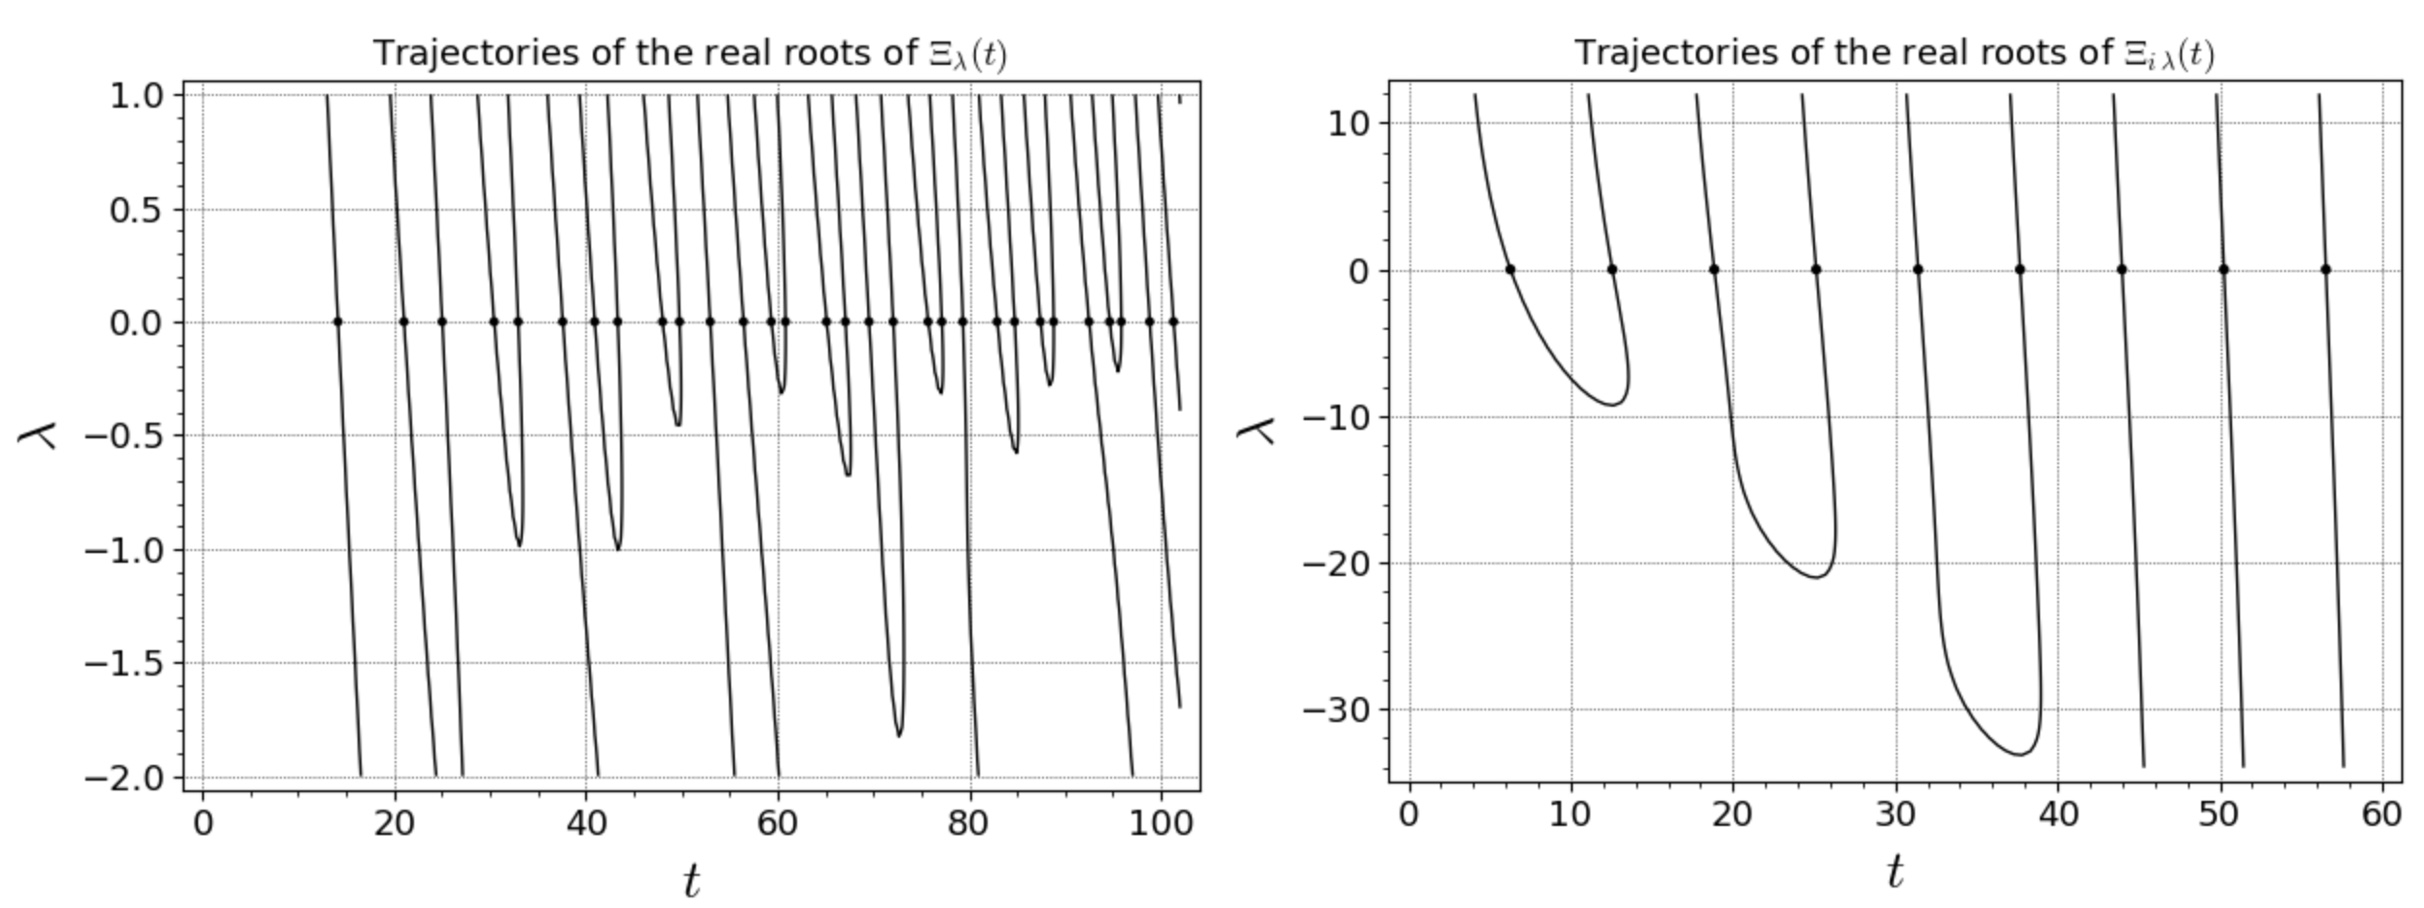
\includegraphics[width=1\linewidth]{PolyaDeBruijnFlowdouble.jpg}
  \caption{The graphs show the Pólya-De Bruijn flows of real zeros of $\Xi_{\lambda}(t)$ (left) and $\Xi_{i\,\lambda}(t)$ (right). Some collisions between the trajectories occur when $\lambda < 0$. The collision point is where the real zeros transform into a complex pair when going further back in 'time'. The RH is equivalent to no collisions occurring for $\lambda \ge 0$, which is clearly true for $\Xi_{i\,\lambda}(t)$. The concept of "hyperbolicity", i.e. the preservation of the reality of the zeros when time-parameter $\lambda$ become more positive, is visible in both flows. Observe that from eq. \ref{cfbruijn}, it follows that any collision point of zeros is necessarily (but not sufficiently) at $(t,\lambda)$ where $\frac{d}{dt} \Xi_{i\,\lambda}(t) =0$. From the definition of erf in DLMF, formula 7.2.1, one sees that this occurs if and only $t$ is an integer multiple of $2\pi$. These values of $t$ are also precisely the zeros of $\Xi_{i\,0}(t)$. The right hand plot suggests that the collision points of real zeros are at $t$ where $t$ is an integer multiple of $4\pi$ and that for given $t=4 k \pi$, they occur only for one negative value of $\lambda$ which is asymptotically equal to $-4k \pi$.}
  \label{fig:poldebruijnflow}
\end{figure}
A few facts about the flow of $\Xi_{\lambda}(t)$:
\begin{itemize}
  \item De Bruijn and Newman showed that there exists a constant $\Lambda$, now known as the De Bruijn-Newman constant, at which all zeros will be real and that this is also true for all $\lambda > \Lambda$. During the last decades, good progress has been made on the improvement of the lower bound of $\Lambda$, but little on the upper bound.
  \item In 2018 Tao and Rodgers \cite{rot} proved Newman's lower bound conjecture that $\Lambda \ge 0$, They used techniques from Random Matrix theory to predict the 'time to cool down' and compared this to known facts about the distribution of zeros at $\lambda = 0$. A student of Tao, Alex Dobner later found a much simpler proof \cite{dob} that $\Lambda \ge 0$ which avoids the heat equation approach. Dobner’s approach instead relies on a Riemann-Siegel type approximation for $\Xi_{\Lambda}(t)$ in order to demonstrate the existence of zeros off the critical line.
   \item The prime objective of the 2018 Polymath15 project \cite{pol}, was to lower the upper bound. This was successfully accomplished through a combination of analytic proof, existing numerical verification of the RH up to a certain height and advanced computer calculations. The new upper bound became $\Lambda \verifiedeq 0.22$. After further numerical verification of the RH by Platt et al \cite{pla}, it has now been proven that the upper bound of the De Bruijn-Newman constant is $\lambda \le 0.2$. Hence, a breach of the RH would imply that there exists some pair complex zeros at a certain $T$ that collide in the region $0 \le \Xi_{\lambda}(t) \le 0.2$.
  \item For increasingly positive $\lambda$ we know that the trajectories of zeros "cool down" into a deterministic arithmetic progression that is now well understood. Increasingly negative $\lambda$ will induce more pairs of complex zeros that eventually will organise themselves on deterministic curves. A sparse, but regular set of real zeros (see the $1$-st and $6$-th trajectories in the graph) remains real 'forever'. 
\end{itemize}

\pagebreak

\section{Mathematical considerations}\label{mathcons}
The functions $\Xi(t)$ and $\Xi_i(t)$ need to comply with the following:
\begin{enumerate}
\item Its expansion has to be convergent everywhere in $\mathbb{C}$.
\item Fubini's theorem should hold when swapping summation and integration.
\item All zeros in the flow must be simple to ensure their first derivative is $\ne 0$.
\item For Hadamard factorisation, the flow must be even, non-zero at the origin and entire of order $1$. 
\end{enumerate} 

The disadvantage of our generic approach is that the Riemann $\Xi(t)$ function appears in the coefficients. This makes the task of providing a rigorous proof for 1) and 2) more difficult. Romik showed in his paper how to derive simpler expressions for the coefficients that enable a rigorous proof of 1) and 2) and also pave the way for deriving their asymptotics. Following the same techniques, we managed to generalise his approach towards a broader set of parameters for Meixner-Pollaczek and Continuous Hahn families. We also found similar expressions for the coefficients of the Generalised Laguerre, Continuous Dual Hahn and Wilson polynomials, albeit for the latter two for $\Xi'(t)/t$ and $\Xi(0) \pm \Xi(t)$ and with a restricted set of parameters. We've captured these in appendix \ref{specexpansions}. Since this approach does not allow for a free choice of parameters of each family that we aim to visualise, and our domain of interest is $t < 60$, we decided to just assume that 1) and 2) to be true at this stage.

For $\Xi(t)$ it is still an open problem whether all its zeros are simple, however in our domain of interest $t < 60$ this is true. Also, it is known that 4) holds for $\Xi(t)$ and $\Xi_i(t)$.

Note that to properly compare the new Poisson flows with the Polya-De Bruijn flow, the latter should be vertically "flipped" ($\lambda = -\lambda$) (since we use  $\exp(-r)$.

\section{Computational considerations}\label{compcons}
Visualising the Poisson flow of the Riemann $\Xi$ and $\Xi_i$-functions requires a significant amount of evaluations of the function itself as well as the hypergeometric functions associated with the family of orthogonal polynomials. During the Polymath15 project we discovered that with modern software and hardware evaluating $\Xi$ actually has become quite tractable at smaller heights (p16, remark 4.1 of \cite{pol}). 

The most intense task is to pre-compute and store the coefficients (for each set of polynomial parameters) that are independent of $t, r$. This once-off computation makes the evaluation of the flow $X^\phi_r(t)$ significantly faster since only one hypergeometric function remains. For both steps we have used the advanced FLINT/ARB C-library for arbitrary-precision ball arithmetic \cite{arb}. We have also considered using pari/gp and, although much easier to code, it proved to be slower and lacks some of the more advanced hypergeometric functions (${}_3F_2,{}_4F_3$) that we need.

For the pre-computation step we require the full FLINT/ARB C-library and especially the multi-threaded function for the fast evaluation of the integral. This multi-threaded function seems not (yet) available in the 'wrapped', easier readable, version of FLINT/ARB under SageMath, hence we coded it all in "plain ARB". For the flow visualisation step, we make use of Sagemath \textit{implicit plot} function that automatically plots where the contour of a function vanishes. There is no longer a need for dedicated root finding routines and this again speeds up computations considerably. To allow for easy integration between evaluating and plotting the Poisson flow, we made use of the "wrapped" version of FLINT/ARB under SageMath.    

To keep a decent balance between gaining sufficient visual insights and the amount of computations required, we decided to compute the flows up to $t=60$ which comprises the flows of the first $13$ ordinates of the non-trivial zeros of $\Xi(t)$ at $r=0$. Our target accuracy at $t=60, r=0$ is $20$ digits, which allows for some contingency to 'peek' beyond that point. The key tuning parameters to achieve this accuracy are the number of pre-computed coefficients, the precision settings in the software and the finite limits of the integrals/sums involved. Finding the right settings was done heuristically. 

For the hardware we have used an Apple Mac Studio, M2 ultra, 64Gb, using all its 24 cores to the max. All documented software, including the accuracy settings that we have used to pre-compute the coefficients and to produce the visuals, is available from our GitHub \cite{git} repository. All pre-computed coefficients and other relevant data are stored there as well.
\pagebreak
\section{Verifying the results}\label{checks}
We have implemented the following checks to ensure the computations were done correctly:

\begin{enumerate}
\item \textit{Ensure the code produces replicable results.} We verified the correct working of our FLINT/ARB code by fully reproducing it in Maple\texttrademark  \cite{map} and comparing randomly chosen values. 
\item  \textit{Verify the expansion meets the target accuracy of $20$ digits.} Check that the difference $F(60)-X^\phi_0(60)$ shows at least $20$ zeros.
\item  \textit{Verify the expansion has been done correctly.} Check that $F(t) \verifiedeq \sum_{n=0}^\infty (\text{coefficient}_n)$ at $t=0$ (Hermite and Laguerre) and at $t\verifiedeq ai$ (Meixner-Pollaczek, Continuous Hahn, Continuous Dual Hahn and Wilson polynomials). 
\item \textit{Verify that the derived expressions for $\frac{d}{d\,r}z_k(r)$ work correctly.}. Check that the Newton approximation of the first derivative at a known $k$-th zero of $F$ at $r=0$, equals the value of the derived equation for $\frac{d}{d\,r}z_k(0)$. For brevity let $z_n = z_n(0)$. 

For the PDEs we evaluate the sum of zeros for $F=\Xi(t), z_n=\Im(\rho_n)$ and $F=\Xi_i(t), z_n=2\pi n$ respectively as:

\begin{align}
 \sum_{j \ne k}^{'} \frac{1}{z_k-z_j} &\verifiedeq \left(\sum_{j =1}^{k-1} \left(\frac{1}{z_k-z_j}\right)+\left(\frac{1}{z_k+z_j}\right)\right) +\left(\sum_{j = k+1}^{100000} \left(\frac{1}{z_k-z_j}\right)+\left(\frac{1}{z_k+z_j}\right)\right)+\left(\frac{1}{2\,z_k} \right) \notag \\
  \sum_{j \ne k}^{'} \frac{1}{z_k-z_j} &\verifiedeq -\frac{1}{2\pi k} \notag
\end{align}

For the DDEs we evaluate the product of zeros $F\verifiedeq \Xi(t), z_n=\Im(\rho_n)$ and $F=\Xi_i(t), z_n=2\pi n$ respectively as (note: $c \verifiedeq \pm 1$ or $c =\pm i$):

\begin{align}
 \prod_{j \ne k}^{'} \frac{z_k+c-z_j}{z_k-z_j} &\verifiedeq c\,\left(\prod_{j =1}^{k-1} \left(1+\frac{c}{z_k-z_j}\right)\,\left(1+\frac{c}{z_k+z_j}\right)\right)\,\left(\prod_{j = k+1}^{100000} \left(1+\frac{c}{z_k-z_j}\right)\,\left(1+\frac{c}{z_k+z_j}\right)\right)\,\left(1+\frac{c}{2\,z_k} \right) \notag \\
 \prod_{j \ne k}^{'} \frac{z_k+c-z_j}{z_k-z_j} &\verifiedeq 2\,k\,\pi\,c^4\,(-1)^k\,\frac{\sin\left(\pi\,k+\dfrac{c}{2}\right)}{\pi\,k+\dfrac{c}{2}} \notag
\end{align}
\end{enumerate}

\section{Overview of the results and observations} \label{results}
We have demonstrated that visualising the Poisson flows is computationally tractable at limited heights (say $t < 100$). The visualised flows could provide potentially new perspectives on the evolution of the real zeros of $\Xi(t)$ and $\Xi_i(t)$ as well as their governing laws.

In appendix \ref{eqsused}, we list all relevant equations for each orthogonal polynomial family in scope. The visuals of the flows for a specific set of parameters are also included there. In support of our conclusions below, we did produce much more data using different parameters to understand the impact on the flows and the asymptotics of the coefficients (data is available on our github \cite{git}). 

\subsection{Some generic observations}

We begin with a realistic one: all Poisson flows share a common characteristic. At  $r = 0$, these flows exhibit a distortion or approximation of the original functions  $\Xi(t)$  and  $\Xi_i(t)$ , where the complexity appears to be at its highest. As  $r$  evolves over ‘time,’ we observe information seemingly flowing away from  $r = 0$  toward later or earlier phases. In these less complex, ‘distorted’ domains ($ r \ne 0$ ), the trajectories either collide or converge toward an arithmetic progression. Unfortunately, this ‘distorted’ domain does not (yet) provide any additional insights into the distribution of the zeros at  $r = 0$.

However, on a more positive note, we find it encouraging to see that there appear to be two types of flows for $F$, at least for smaller parameters say $<1$. \textit{Type A:} Collisions seem to occur when $r > 0$: Polya-De Bruijn, Hermite and Generalised even Laguerre flows. \textit{Type B:} No collisions seem to occur when $r > 0$: Meixner-Pollaczek, Continuous Hahn, Continuous Dual Hahn and Wilson. All type A flows are driven by PDEs (and sums of zeros) and all type B flows by DDEs (and products of zeros). Both worlds are only connected through the two limit relations; between the Meixner-Pollaczek and the Generalised even Laguerre family (eq. (9.7.14) in \cite{koe}) and between the Meixner-Pollaczek and Hermite family (eq. (9.7.15) in \cite{koe}). 

In the table \ref{tab:tablefindings} we summarize the observed behaviour of the expansion coefficients (i.e. whether they are always positive/negative/alternating and/or increase/decrease monotone).
\begin{table}[H]
  \begin{center}
    \caption{Overview of our findings ordered by flow type (for small parameters only)}
    \label{tab:tablefindings}
    \begin{tabular}{|l|c|c|l|} 
      \hline
     Flow & Type & Dynamics & Coefficients\\
      \hline
      & & & \\
      $X^\mathcal{PB}_{\lambda}(t)$ & A & PDE &\\
      $X^\mathcal{H}_r(t)$  & A & PDE & Odd index $= 0$, all positive real, monotone decreasing\\
      $X^\mathcal{L}_r(t)$  & A & PDE & All positive real, monotone decreasing\\
      & & & \\
      $X^\mathcal{MP}_r(t)$  & B & DDE & Odd index $= 0$, all positive real, monotone decreasing\\
      $X^\mathcal{CDH}_r(t)$  & B & DDE & All positive real, monotone decreasing\\
      $X^\mathcal{CH}_r(t)$  & B & DDE & Odd index $= 0$, all positive real, monotone decreasing\\
      $X^\mathcal{W}_r(t)$  & B & DDE & All positive real, monotone decreasing\\
      & & & \\
      \hline
    \end{tabular}
  \end{center}
\end{table}

We observe that when the parameters of a family are increased beyond the domain  $> 1$ , the coefficients no longer exhibit a monotonic decrease. Instead, the initial coefficients tend to increase rapidly and/or fluctuate for a period (also negatively) before eventually resuming the monotonic decreasing pattern. To illustrate this behaviour for the Meixner Pollaczek family, in Figure \ref{fig:MeixCoeff} we plotted the coefficients for different values of parameter $a$.

\begin{figure}[H]
  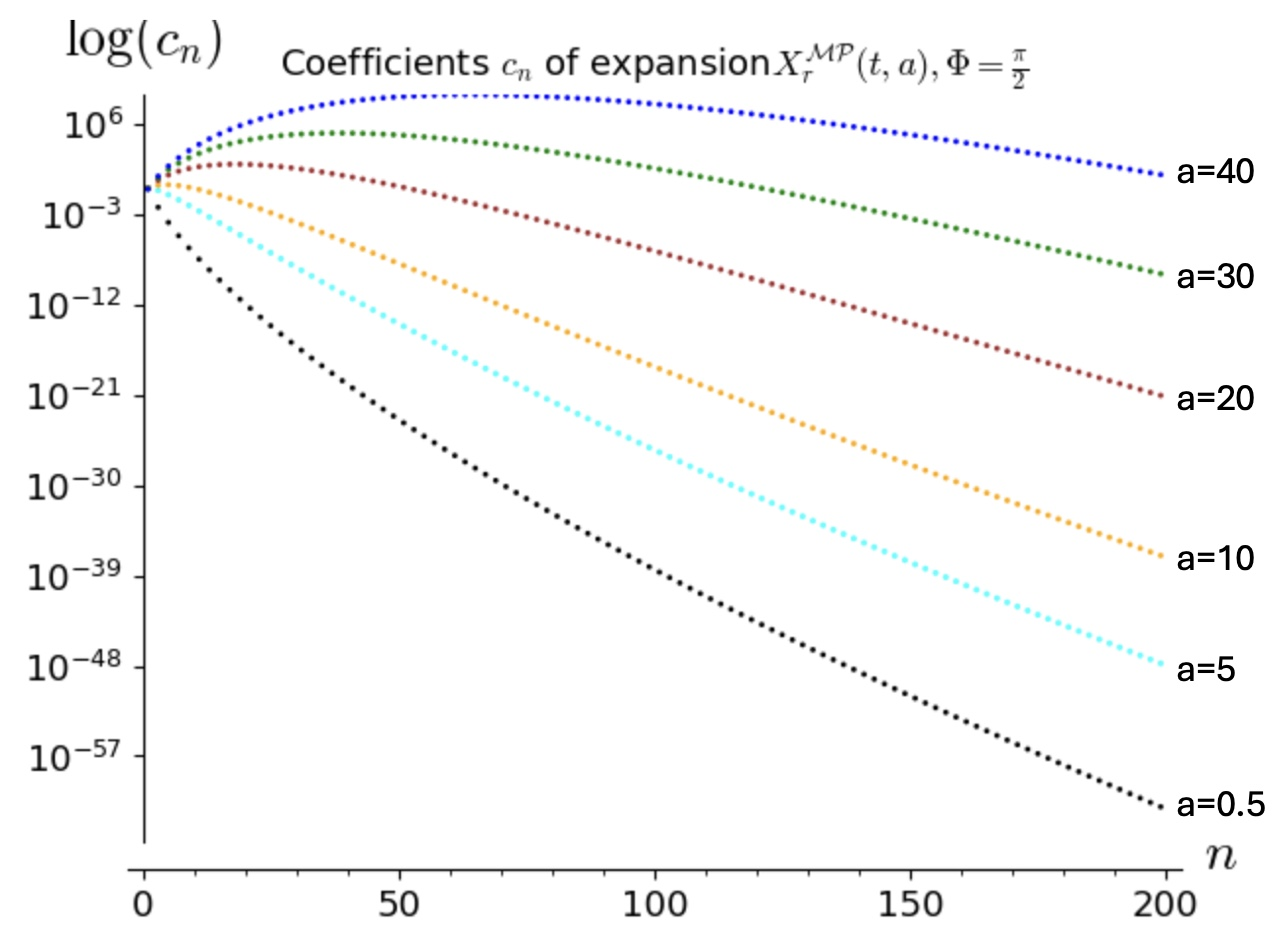
\includegraphics[width=0.8\linewidth]{MeixCoeff.jpg}
  \caption{When parameter $a$ is increased, we can clearly see a significant "hump" is induced in the first set of coefficients of the expansion. This "hump" will become higher and its tail longer for larger $a$. Observe that for $a$ small, say $\frac12$, we see a monotonic decreasing set of coefficients, without any 'hump'. Note that $c_{2n+1}=0$, hence the small gaps between the dots.}
  \label{fig:MeixCoeff}
\end{figure}   

In the next two sections, we take a deeper dive into the type A (Generalised even Laguerre) and type B flows.

\subsection{Specific observations about the Generalised even Laguerre flow}

We observed from Figure \ref{fig:flowL} that the trajectories of the real zeros rotate anti-clock wise when $\alpha$ is increased and vice versa. This raises the question at which $\alpha$ the trajectory will be fully vertical i.e. when $\frac{\mathrm{d}}{\mathrm{d} r} z_k(0) = 0$.

The equation (\ref{zerodiff}):

\begin{equation}
\frac{\mathrm{d}}{\mathrm{d} r} z_k(r)\verifiedeq-\sum_{j \ne k}^{'} \frac{1}{z_k(r)-z_j(r)} -\frac{\alpha+\frac12}{z_k(r)}+z_k(r))
\end{equation}

allows us to find the value for $\alpha$ where $\frac{\mathrm{d}}{\mathrm{d} r} z_k(r) = 0$. Since we know the (ordinates of) zeros at $r=0$ for both $F= \Xi(t)$ and $F= \Xi_i(t)$ and can use those to compute the (finite) sum. For $\Xi(t)$ we have used the first $300.000$ ordinates of the non-trivial zeros that provides a sufficiently accurate approximation (at approx. 2-3 decimal points). For the zeros of $\Xi_i(t)$ we have the closed form \ref{zeroclosed}. The graphs on the next page visualise how the trajectories curve backwards when $\frac{\mathrm{d}}{\mathrm{d} r} z_k(0) = 0$ for a selected $k$, and eventually hit the $r$-axis at $t=0$. 

\small{
\begin{table}[H]
  \begin{center}
    \caption{$F\verifiedeq\Xi(t)$}
    \label{tab:tablefunc}
    \begin{tabular}{|c|c|c|} 
      \hline
       & &\\
      $k$ & $z_k$ & $\alpha$ where $\frac{\mathrm{d}}{\mathrm{d} r} z_k(0) = 0$ \\
       & \\
      \hline
       & &\\
      $ 1$ & $14.134725141 $ &$207.47977679$ \\ 
      $ 2$ & $21.022039638 $ &$457.28973963$ \\ 
      $ 3$ & $25.010857580 $ &$639.68392465$ \\ 
       & & \\
       \hline
    \end{tabular}
  \end{center}
\end{table}
}

\begin{figure}[H]
  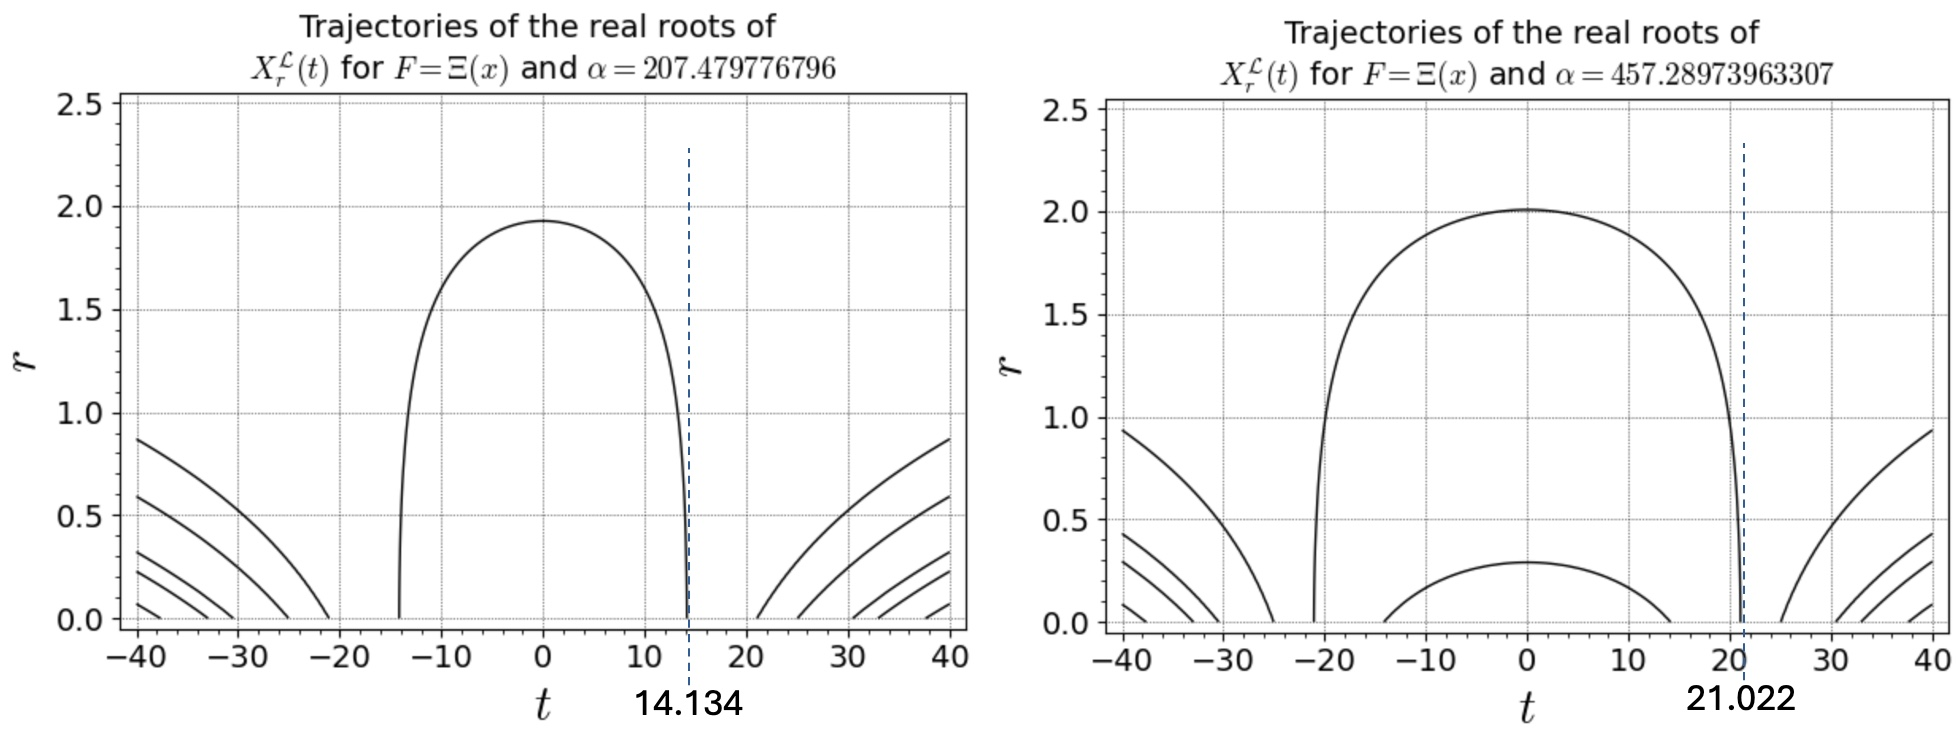
\includegraphics[width=1\linewidth]{LaguerreCurvedXi.jpg}
  \caption{It appears that for subsequent $z_k$, the associated $\alpha$ bends the curves backwards sequentially (so, first $z_1$, then $z_2$, etc.). }
  \label{fig:flowLcurveXi}
\end{figure}


\small{
\begin{table}[H]
  \begin{center}
    \caption{$F\verifiedeq\Xi_i(t)$}
    \label{tab:tablefunc}
    \begin{tabular}{|c|c|c|} 
      \hline
       & &\\
      $k$ & $z_k$ & $\alpha$ where $\frac{\mathrm{d}}{\mathrm{d} r} z_k(0) = 0$ \\
       && \\
      \hline
       & &\\
      $ 1$ & $2\,\pi $ &$\,\,\,4\,\pi^2 + 1/2$ \\ 
      $ 2$ & $4\,\pi $ &$16\,\pi^2 + 1/2$ \\ 
      $ 3$ & $6\,\pi $ &$36\,\pi^2 + 1/2$ \\ 
       & &\\
       \hline
    \end{tabular}
  \end{center}
\end{table}
}

\begin{figure}[H]
  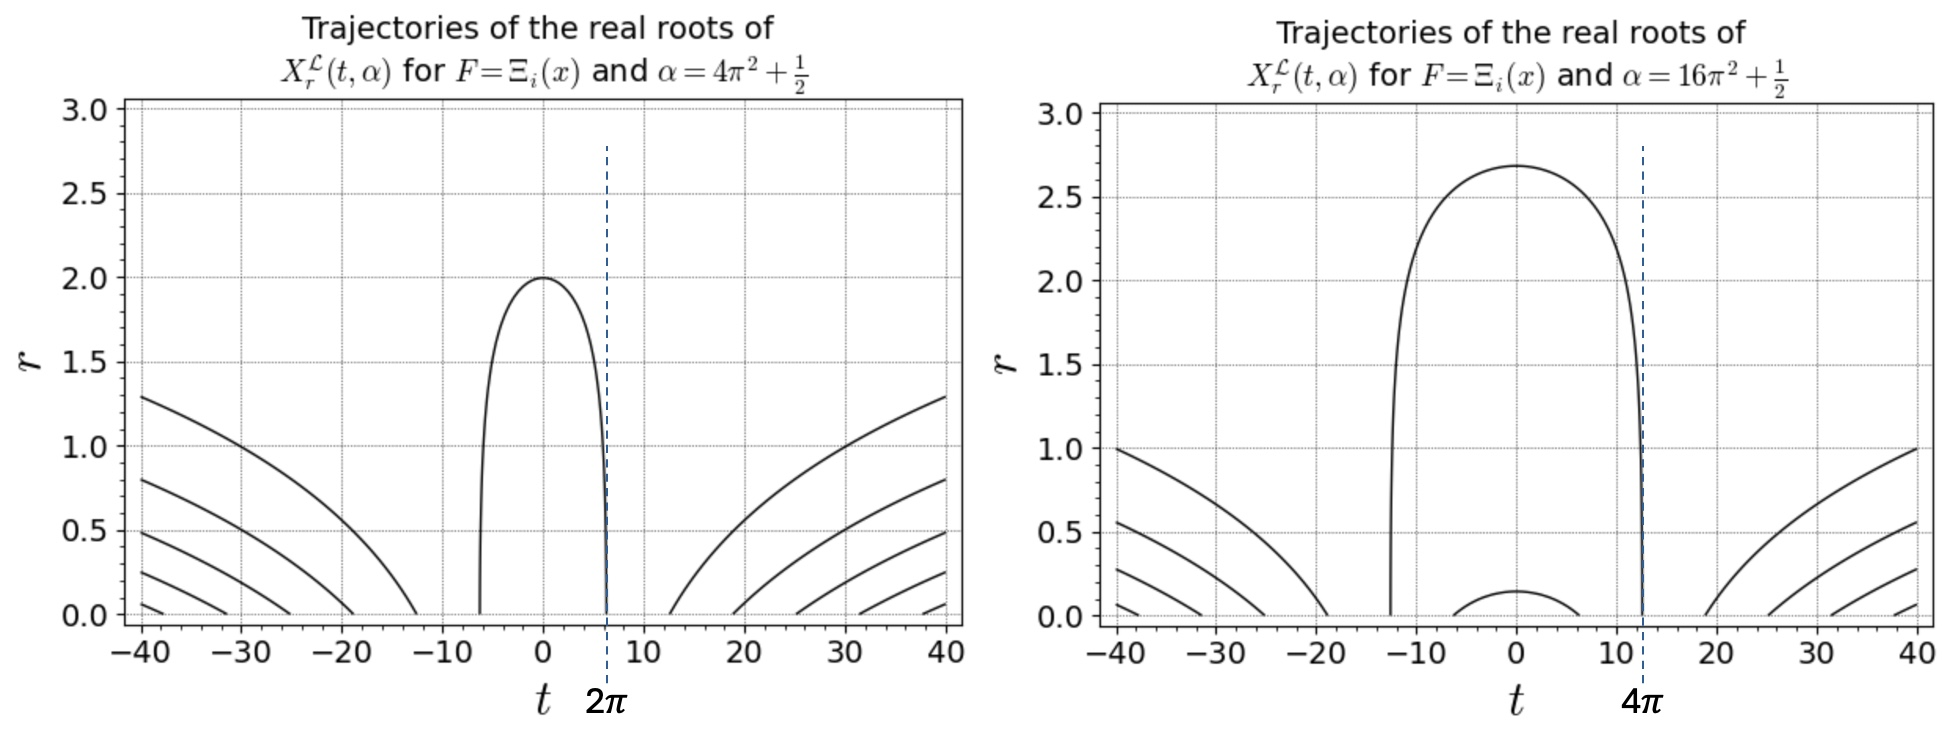
\includegraphics[width=1\linewidth]{LaguerreCurvedXii.jpg}
  \caption{It appears that for subsequent $z_k$, the associated $\alpha$ bends the curves backwards sequentially (so, first $z_1$, then $z_2$, etc.). }
  \label{fig:flowLcurveXii}
\end{figure}

For $r > 0$, it is difficult to analytically find collisions between trajectories of real zeros, i.e. those locations where $\frac{\mathrm{d}}{\mathrm{d} r} z_k(r) = 0$ and we have maxima or minima. There is something else could verify though:

\begin{lemma} \label{LagisPB} The following relation exists between the Laguerre, Hermite and Pólya- DeBruijn flows:

\begin{equation}
X^{\mathcal{L}}_r\left(t;-1/2\right) = X^{\mathcal{H}}_r\left(t\right) = X^{\mathcal{PB}}_{\tfrac{\exp(-2r)-1}{4}}\left(\exp(-r)\,t\right) 
\end{equation} 
\end{lemma}
\begin{proof}
This was already proven by Romik (eq. 2.51 of \cite{rom}) for the Hermite flow, however we follow a different approach. We temporarily switch back to $r^{2n}$ instead of $\exp(-2nr)$ and therefore have the Laguerre flow as:
\begin{equation}
  X^{\mathcal{L}}_r(t;\alpha)\left[F(t)\right] \verifiedeq \sum_{n=0}^\infty \gamma_n(\alpha)\,{}_1F_1\left(-n, \alpha+1,t^2\right)\,r^{2n}
\end{equation}
Now, take the Poisson kernel and apply the Hardy-Hille formula to obtain its closed form:
\begin{align}
  p^\mathcal{L}_r(x,y, \alpha) &= \sum_{n=0}^\infty \frac{2\,n!}{\Gamma(a+n+1)}\,\hat{L}^{\alpha}_n(x)\,\hat{L}^{\alpha}_n(y)\,r^{2n} \\
  &=2\,\frac{\left((x y r)^2\right)^{-\alpha/2}}{1-r^2}\,\exp\left(-\frac{(x^2+y^2)\,r^2}{1-r^2}\right)\,\text{BesselI}\left(\alpha, 2\,\frac{x y r}{1-r^2}\right) \label{lagpoiclosed}
\end{align}
The Poisson flow can now also expressed as: 
\begin{align}
X^{\mathcal{L}}_r(t;\alpha) &\verifiedeq \int_0^\infty F(x)\,p^\mathcal{L}_r(x,y)\,w_x(\alpha) \,\mathrm{d} x \\
   &\verifiedeq \int_0^\infty F(x)\,2\,\frac{\left((x y r)^2\right)^{-a/2}}{1-r^2}\,\exp\left(-\frac{(x^2+y^2)\,r^2}{1-r^2}\right)\,\text{BesselI}\left(\alpha, 2\,\frac{x y r}{1-r^2}\right)\,\exp(-x^2)\,x^{2\alpha+1} \,\mathrm{d} x
\end{align}
For $\alpha = -1/2$, the Bessel-function has a closed form and after some clean-up the flow becomes:
\begin{align}
X^{\mathcal{L}}_r(t;-1/2) &= \int_0^\infty F(x)\,\frac{2\,i\,\exp\left(\frac{(x^2+y^2)\,r^2}{r^2-1}\right)\,\cosh\left(\frac{2 t x r}{r^2-1}\right)}{\sqrt{r^2-1}\,\sqrt{\pi}}\,\exp(-x^2)\,\mathrm{d} x \\
&= \frac{1}{\sqrt{r^2-1}\,\sqrt{\pi}}\, \int_0^\infty F(x)\,\left(\exp\left(\frac{(r t -x)^2}{r^2-1}\right)+\exp\left(\frac{(r t +x)^2}{r^2-1}\right)\right)\,\mathrm{d} x \\
&= \frac{1}{\sqrt{r^2-1}\,\sqrt{\pi}}\, \int_{-\infty}^\infty F(x)\,\exp\left(-\frac{(r t -x)^2}{1-r^2}\right)\,\mathrm{d} x \\
&= \frac{1}{\sqrt{\pi}}\, \int_{-\infty}^\infty F\left(r t-v \,i\, \sqrt{r^2-1}\right)\,\exp\left(-v^2\right)\,\mathrm{d} v \label{result}
\end{align}
where we used $v = \dfrac{r t -x}{\sqrt{1-r^2}}$. Comparing (\ref{result}) to the Gaussian type integral for the Pólya-DeBruijn flow:
\begin{equation}
X^{\mathcal{PB}}_{\lambda}(t)[F] =   \frac{1}{\sqrt{\pi}}\,\int_{-\infty}^\infty F\left(t - 2\,i\,v\sqrt{\lambda}\right)\mathrm{e}^{-v^2}\mathrm{d}v
\end{equation}
and after reintroducing the mapping $r \mapsto \exp(-r)$, the result follows.
\end{proof}

Lemma \ref{LagisPB} implies that the Laguerre and Hermite flows only cover the range $-0.25 \le \lambda \le \infty$ of the Pólya-DeBruijn flow. From studying the collision plot in Figure \ref{fig:poldebruijnflow} of the latter and some additional computations, we know that the first collision in this restricted domain occurs between the zeros $\Im(\rho_{26}) = 94.651344..$ and $\Im(\rho_{27}) = 95.870634..$ at $t \approx 95.4$ and $\lambda \approx -0.22$. We therefore expect to see this collision reflected in the Laguerre flow at $t \approx 277$ and $r \approx 1.06$. This is indeed what we find in Figure \ref{fig:flowLcoll}.
\begin{figure}[H]
  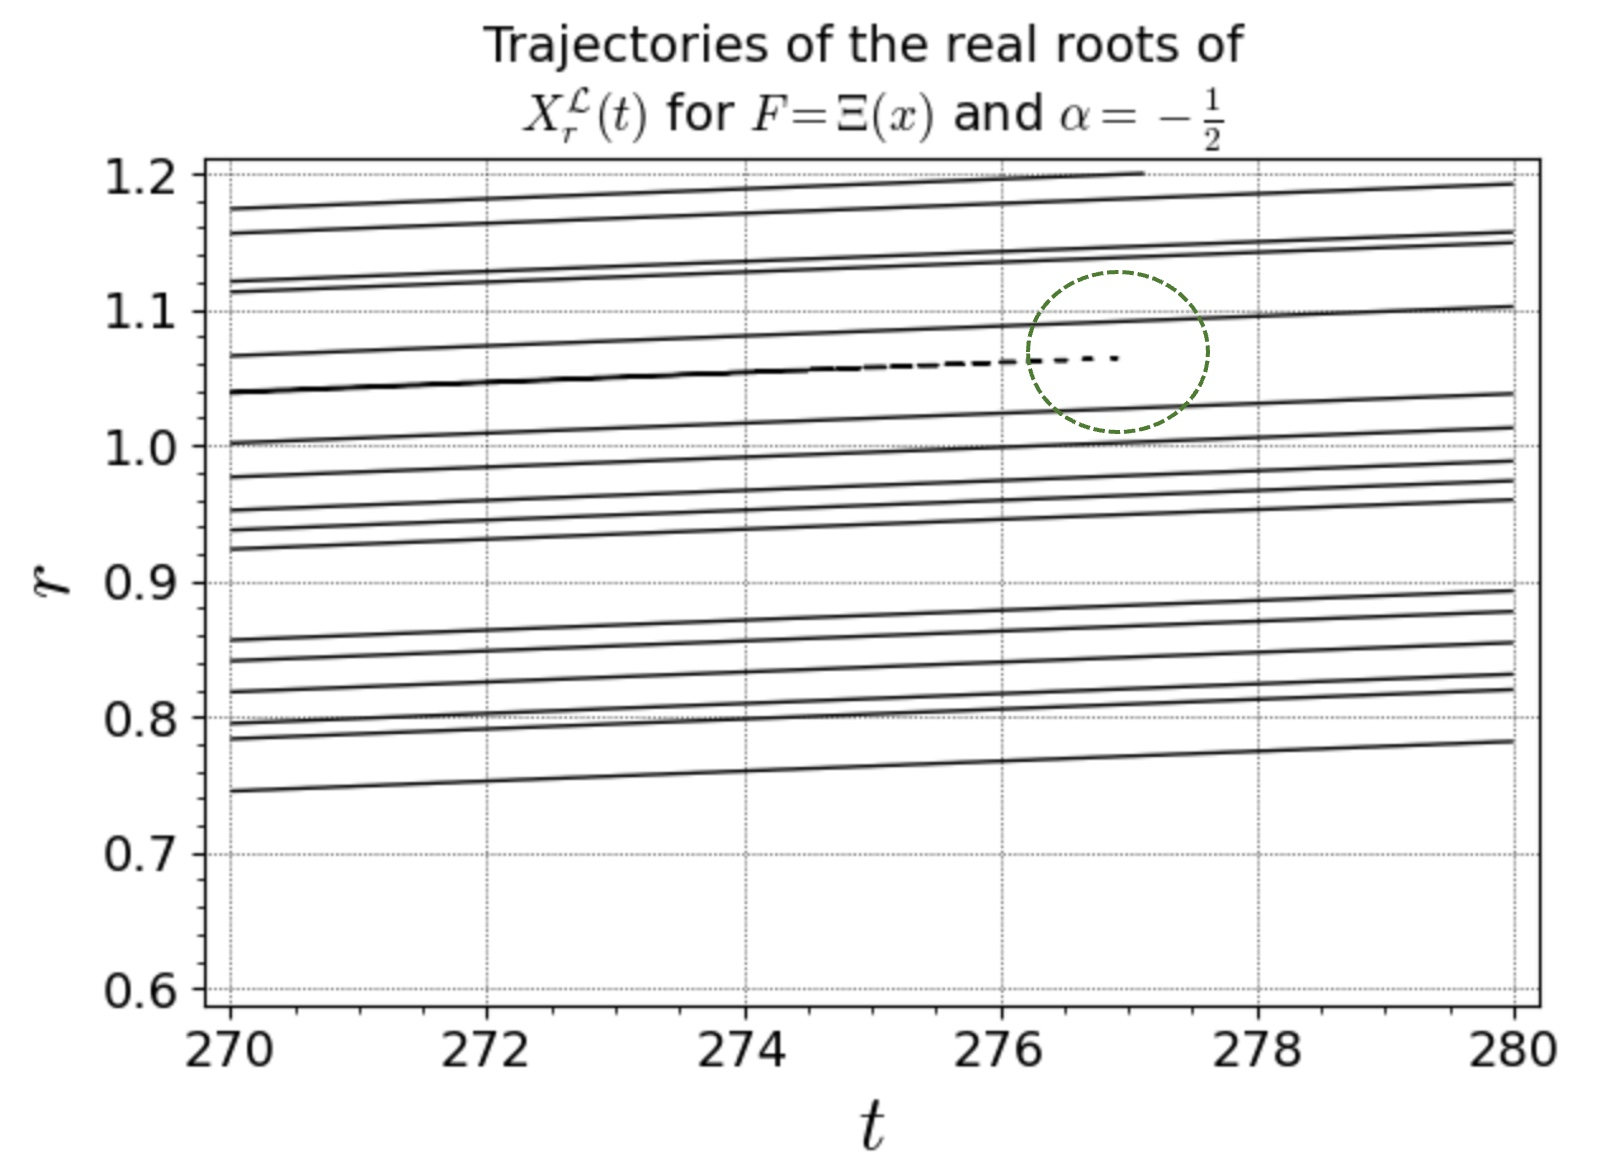
\includegraphics[width=0.7\linewidth]{LaguerreFlowColl.jpg}
  \caption{The collision between zeros $26$ and $27$ as can be seen in Figure \ref{fig:poldebruijnflow} reappears at the expected location in the Hermite flow and this Laguerre flow at $\alpha = -\frac12$.}
  \label{fig:flowLcoll}
\end{figure}

This immediately raises the follow up question on whether this collision continues to exist when $\alpha$ is varied and in particular when $\frac{\mathrm{d}}{\mathrm{d} r} z_{26}(0) = 0$ or $\frac{\mathrm{d}}{\mathrm{d} r} z_{27}(0) = 0$. Figure \ref{fig:flowLcollsplit} illustrates what happens in this case and we observe the collision has fully disappeared. 

\begin{figure}[H]
  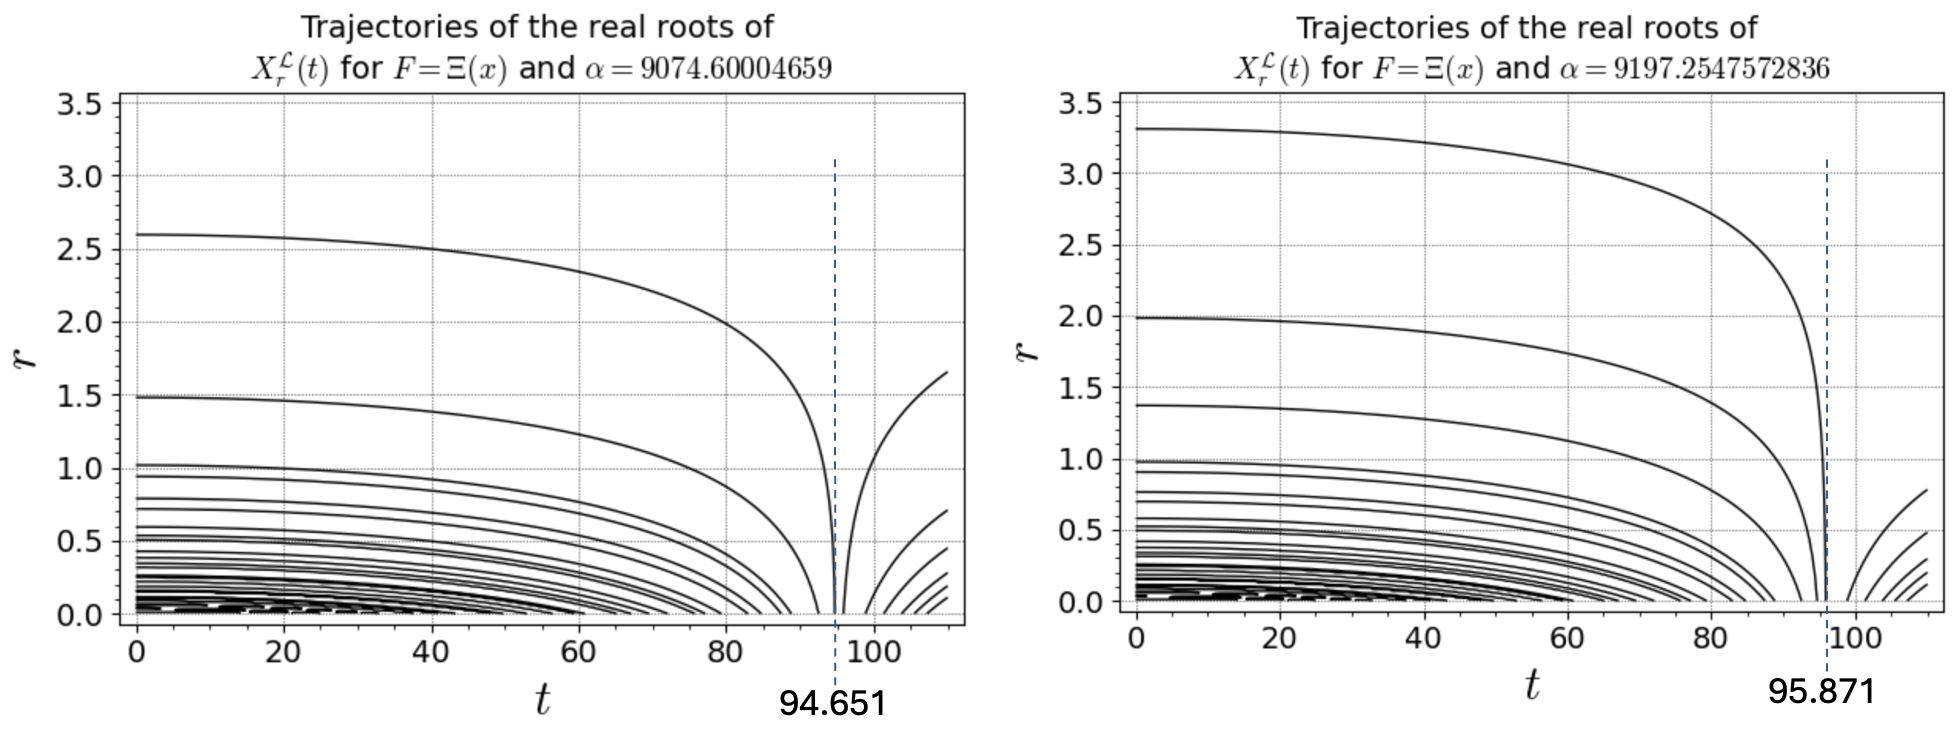
\includegraphics[width=0.9\linewidth]{LaguerreCollSplitdouble.jpg}
  \caption{The trajectories of real zeros when $\frac{\mathrm{d}}{\mathrm{d} r} z_{26}(0) = 0$ (left) or $\frac{\mathrm{d}}{\mathrm{d} r} z_{27}(0) = 0$ (right). Note that the collision between zeros $26$ and $27$ as shown in Figure \ref{fig:flowLcoll} has disappeared at these levels of $\alpha$.}
  \label{fig:flowLcollsplit}
\end{figure}

Based on this observation, it seems that when $\alpha \rightarrow \infty$ all collisions will vanish and all zeros will eventually become real in the domain $r > 0$. Eventually they all appear to gather on the $r$-axis at $t=0$ when $r \rightarrow \infty$. Is there more to about the zeros on the line $t=0$? 

\begin{lemma}
The equation for the even Laguerre flow at $t=0$ is:
\begin{equation}
X^{\mathcal{L}}_r\left(0;\alpha\right) =  \frac{2}{\Gamma(\alpha+1)}\,\int_0^\infty F\left(v\sqrt{1-\exp(-2r)}\right)\,v^{2\alpha+1}\,\mathrm{e}^{-v^2}\mathrm{d}v
\end{equation} 
\end{lemma}
\begin{proof}
For readability reasons we again temporarily switch back to $r^{2n}$ instead of $\exp(-2nr)$. Take the Poisson kernel and apply the Hardy-Hille formula to obtain its closed form:
\begin{align}
  \lim_{y\to 0} \,p^\mathcal{L}_r(x,y,\alpha) &= \sum_{n=0}^\infty \frac{2\,n!}{\Gamma(\alpha+n+1)}\,\hat{L}^{\alpha}_n(x)\,\hat{L}^{\alpha}_n(y)\,r^{2n} \\
  &=\frac{2}{\Gamma(\alpha+1)}\,\frac{\exp\left(-\frac{x^2\,r^2}{1-r^2}\right)}{\left(1-r^2\right)^{\alpha+1}}
\end{align}
The Poisson flow can also be written as: 
\begin{align}
X^{\mathcal{L}}_r(0;\alpha) &\verifiedeq \int_0^\infty F(x)\,p^\mathcal{L}_r(x,y,\alpha)\,w_x(\alpha) \,\mathrm{d} x \\
&\verifiedeq \int_0^\infty F(x)\,\frac{2}{\Gamma(\alpha+1)}\,\frac{\exp\left(-\frac{x^2\,r^2}{1-r^2}\right)}{\left(1-r^2\right)^{\alpha+1}}\,\exp(-x^2)\,x^{2\alpha+1} \,\mathrm{d} x \\
&\verifiedeq \frac{2}{\Gamma(\alpha+1)\,\left(1-r^2\right)^{\alpha+1}}\,\int_0^\infty F(x)\,\exp\left(-\frac{x^2\,r^2}{1-r^2}\right)\,\exp(-x^2)\,x^{2\alpha+1} \,\mathrm{d} x \\
&\verifiedeq \frac{2}{\Gamma(\alpha+1)\,\left(1-r^2\right)^{\alpha+1}}\,\int_0^\infty F(x)\,\exp\left(-\frac{x^2}{1-r^2}\right)\,x^{2\alpha+1} \,\mathrm{d} x \\
&\verifiedeq \frac{2}{\Gamma(\alpha+1)}\,\int_0^\infty F\left(v\sqrt{1-r^2}\right)\,v^{2\alpha+1}\,\mathrm{e}^{-v^2}\mathrm{d}v \label{result3}
\end{align}
where we used $v = \dfrac{x}{\sqrt{1-r^2}}$. 

The result follows after re-introducing the mapping $r \mapsto \exp(-r)$.
\end{proof}

We have used equation \ref{result3} to compute some zeros and we indeed find the ones plotted in Figure \ref{fig:flowLcurveXi} and \ref{fig:flowLcurveXii}. However, we did not observe any pattern nor any rational values (not even for the simpler $\Xi_i$-function). It seems that the complexity of the zeros on the line $r=0$ is still preserved or has become even greater when they reach the line $t=0$. Hence, a possible proof that all zeros on the $r$-axis are all real, seems out of reach.   

\subsection{Specific observations about the type B flows}
For the type B families, we tried to apply a similar trick as in the previous section by computing the free parameter ($a$) at which $\frac{\mathrm{d}}{\mathrm{d} r} z_k(0) = 0$ for a certain $k$. To keep things manageable for the families with multiple free parameters, we kept then all the same. Using equations \ref{zerodiffmp}, \ref{zerodiffch}, \ref{zerodiffcdh} and \ref{zerodiffw}, we obtain the following results for the first 3 zeros:

\small{
\begin{table}[H]
  \begin{center}
    \caption{Solutions for $a$ where $\frac{\mathrm{d}}{\mathrm{d} r} z_k(0) = 0$}
    \label{tab:tablezeros}
    \begin{tabular}{|l|l|c|l|} 
      \hline
       & & &\\
      Polynomial family & Parameters & k & Solution(s) for $a$ where $\frac{\mathrm{d}}{\mathrm{d} r} z_k(0) = 0$ \\
       & & &\\
      \hline
       & & &\\
      Meixner-Pollaczek & $(a, \pi/2)$ & 1 & \,\,\,-21.669631 \\
         &  & 2 & \,\,\,-22.572751 \\
         &  & 3 & \,\,\,-37.543615 \\
       & & &\\
      Continuous Hahn &$(a,a,a,a)$ & 1 & \,\,\,-47.541688, \,\,\,4.202426  \\  
         &  & 2 & \,\,\,-53.418419,  \,\,\,8.272916  \\
         &  & 3 & \,\,\,-82.655321,  \,\,\,7.568091 \\
       & & &\\
      Continuous Dual Hahn &$(a,a,a)$ & 1 & \,\,\,-68.170830, 12.599724, \,\,\,-4.670814\\ 
         &  & 2 & \,\,\,-79.705489, 20.857647, \,\,\,-5.721374 \\
         &  & 3 & -121.785557, 22.209862, \,\,\,-8.317406 \\
       & & &\\
      Wilson &$(a,a,a,a)$ & 1 &\,\,\,-91.458801,   19.302338, -10.350583, 2.184485 \\ 
         &  & 2 & -107.335435,  31.262075, -14.136174, 4.117243 \\
         &  & 3 & -163.574678, 34.039808, -18.376806, 3.824204 \\
       & & &\\
       \hline
    \end{tabular}
  \end{center}
\end{table}
}

Since our expansions require the parameters to be positive, we ruled out the negative solutions for $a$. This implies we cannot apply the approach from the previous section to the Meixner-Pollaczek family. To still obtain some information about this family, we decided to just visualise the flows at increasingly higher $a$ and this yielded some information. In section 3.5 of his paper \cite{rom}, Romik showed numerically that the “hyperbolicity” effect no longer persists for the Meixner-Pollaczek flow (using $a =3/4$). Initially, we did not observe this phenomenon in our visuals at lower $a$, however, when we increase $a$ substantially, the 'hyperbolicity' property clearly vanishes (see figure \ref{fig:MeixHyperbFail}).  

\begin{figure}[H]
  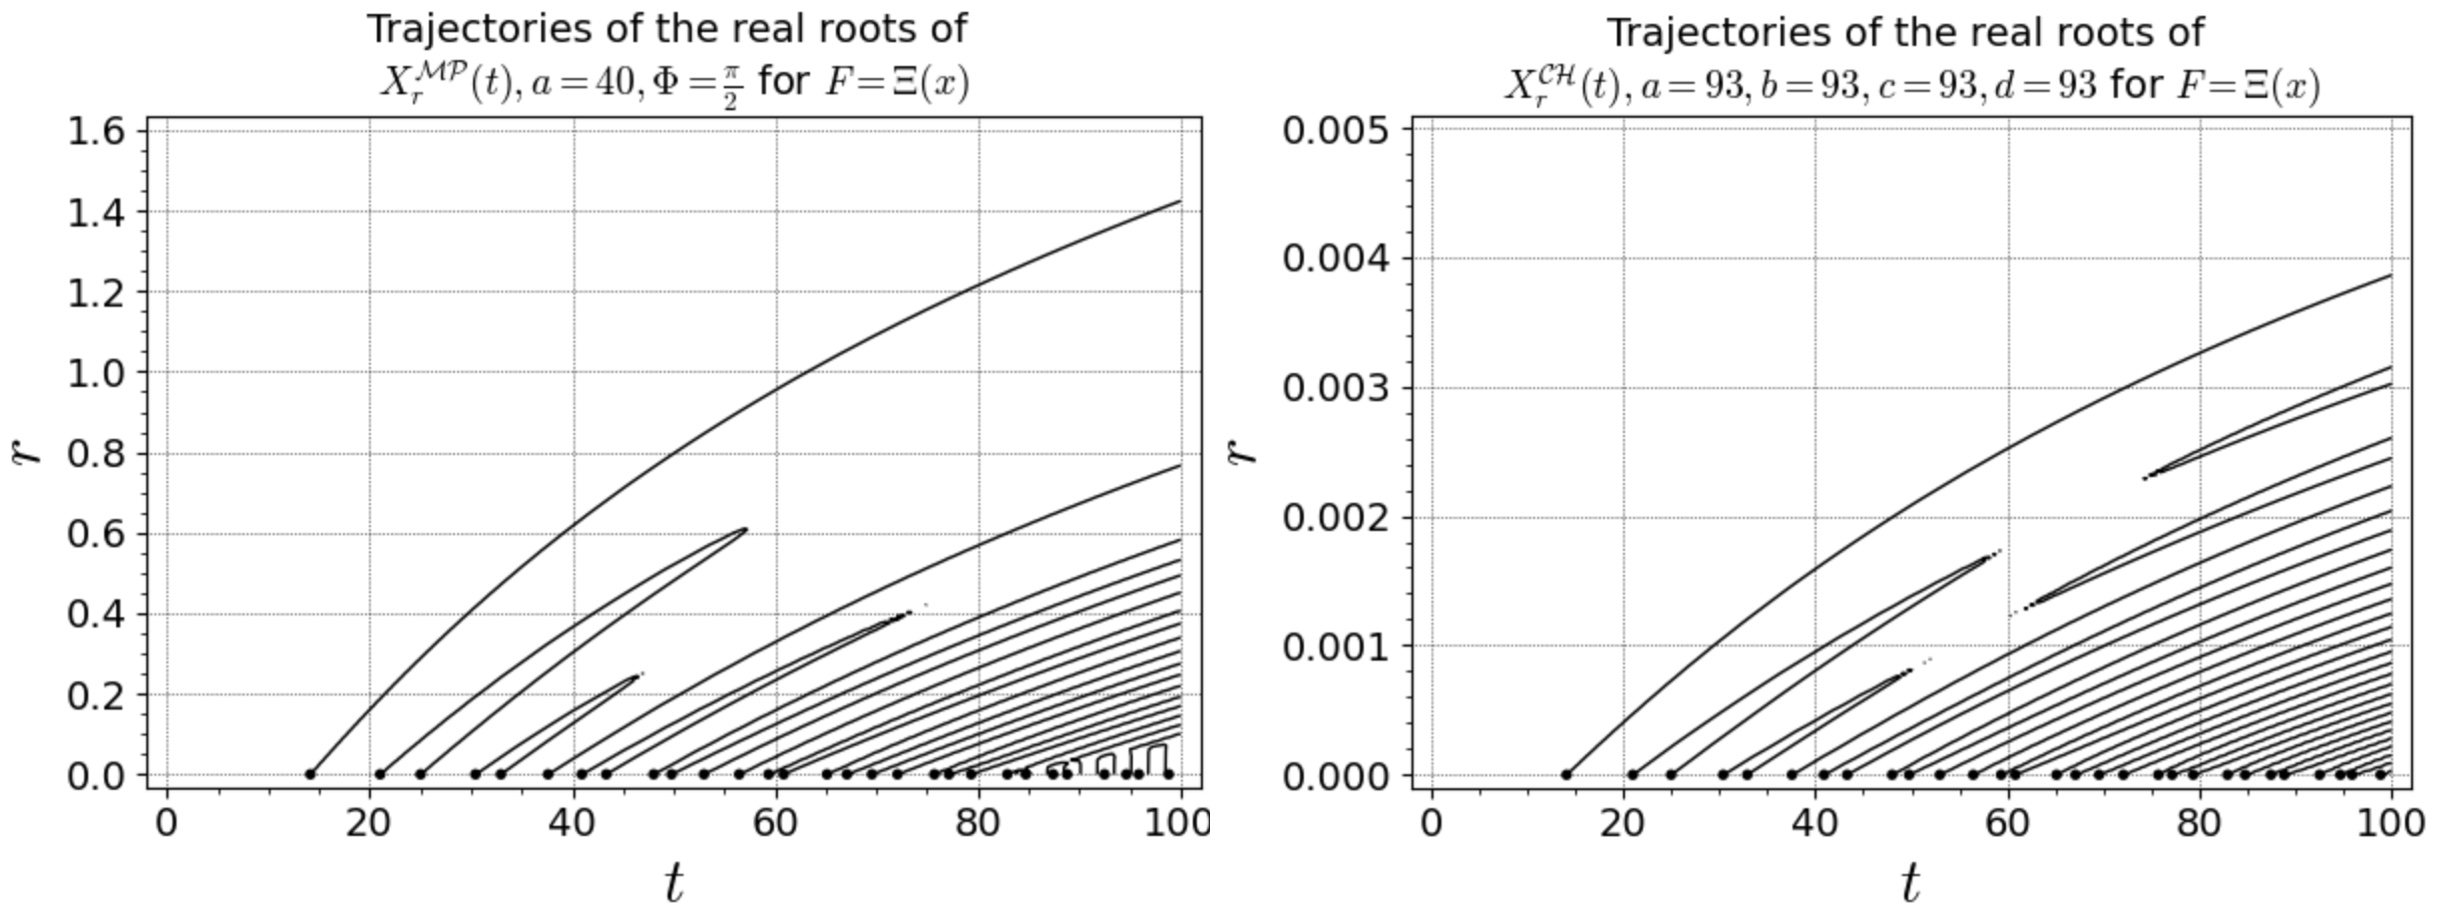
\includegraphics[width=1\linewidth]{MeixPollContHahnbreak.jpg}
  \caption{At lower values of parameter $a$, we still see the 'hyperbolicity' effect in the absence of collisions and the relaxation of the trajectories into some arithmetic progression when $r$ increases. However when $a$ increases, we see collisions occurring in the Meixner-Pollaczek case (left graph) and even multiple collisions emerging in the Continuous Hahn case. Both examples provide a clear indication that the zeros 'once real, do not stay real forever' in these two flows.}
  \label{fig:MeixHyperbFail}
\end{figure}

Table (\ref{tab:tablezeros}) suggests we can compute positive solutions for $a$ for three of the four type B families. To establish whether the trajectories also "bend back" to the $r$-axis, we computed the Continuous Dual Hahn flows at $a=10$ and $a=30$ and indeed find the expected patterns.

\begin{figure}[H]
  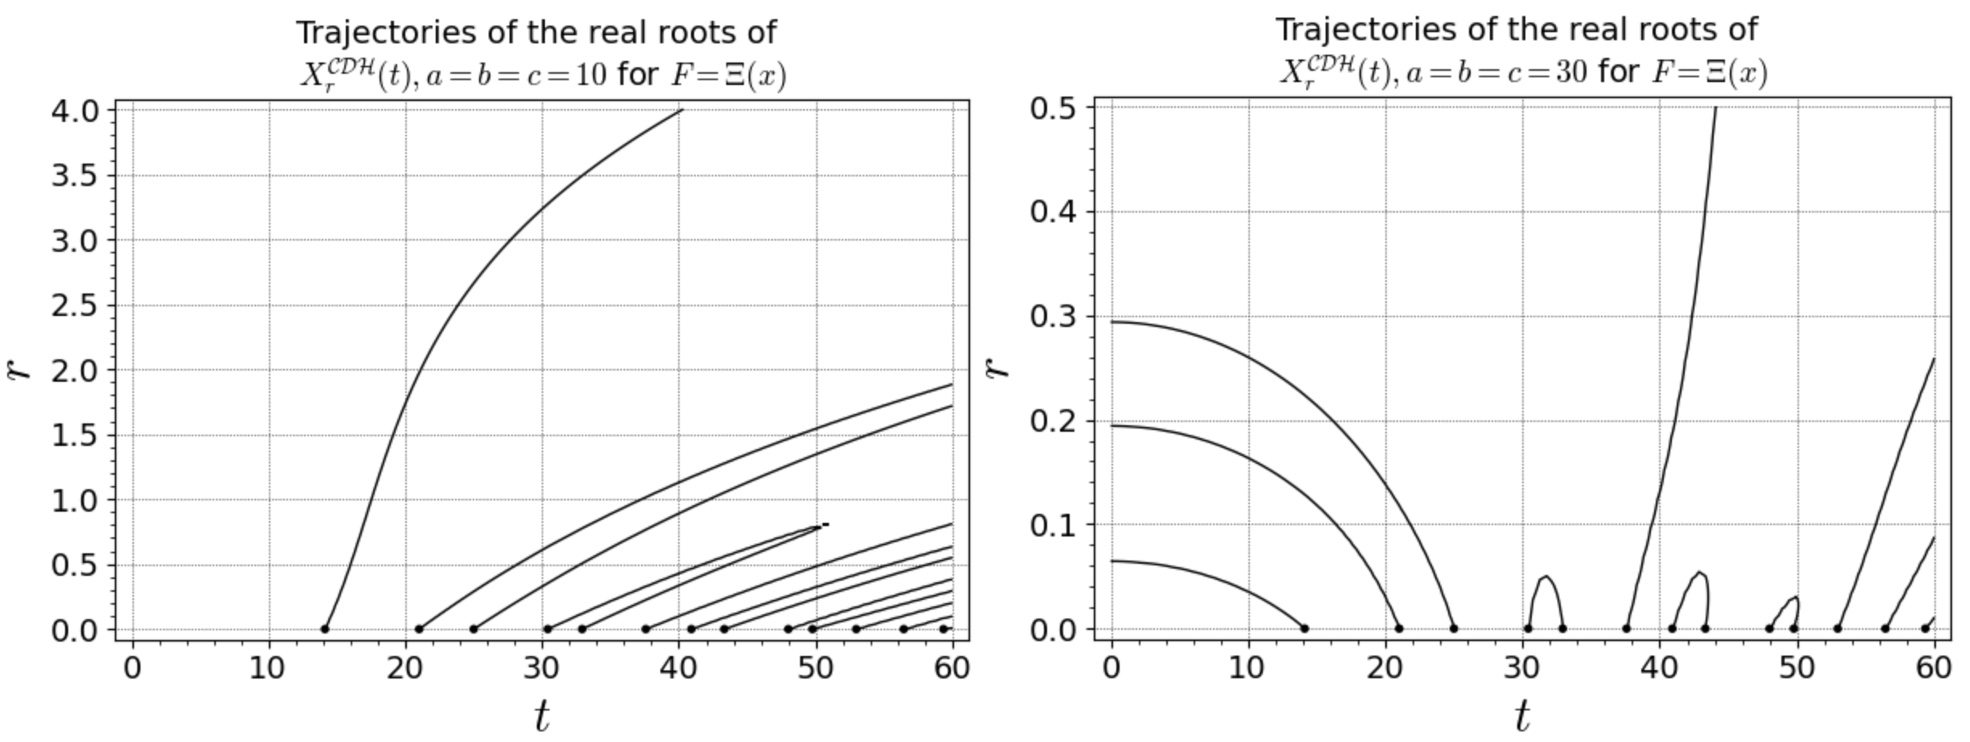
\includegraphics[width=0.9\linewidth]{ContDualHahncolls.jpg}
  \caption{We show the graphs for the Continuous Dual Hahn family for $a=10$ (left) and $a=30$ (right). Similarly to the Laguerre flow, we again see three curves curving towards the $r$-axis in the right panel (since $a=30 > a=22.209862$). In both graphs we also see some collisions emerging. A check of a graph for $a=3$ (not shared), reveals that there do not seem to be any collisions. It appears that, when $a$ increases, we are watching a kind of 'race' between emerging collisions and the backward curves catching up and 'ripping' the collisions apart.}
  \label{fig:ContHahnCurved}
\end{figure}

An interesting case arises from the two solutions for $a$ we find for the Wilson family. The outcomes are visualised in Figure \ref{fig:WilsonCurved}.

\begin{figure}[H]
  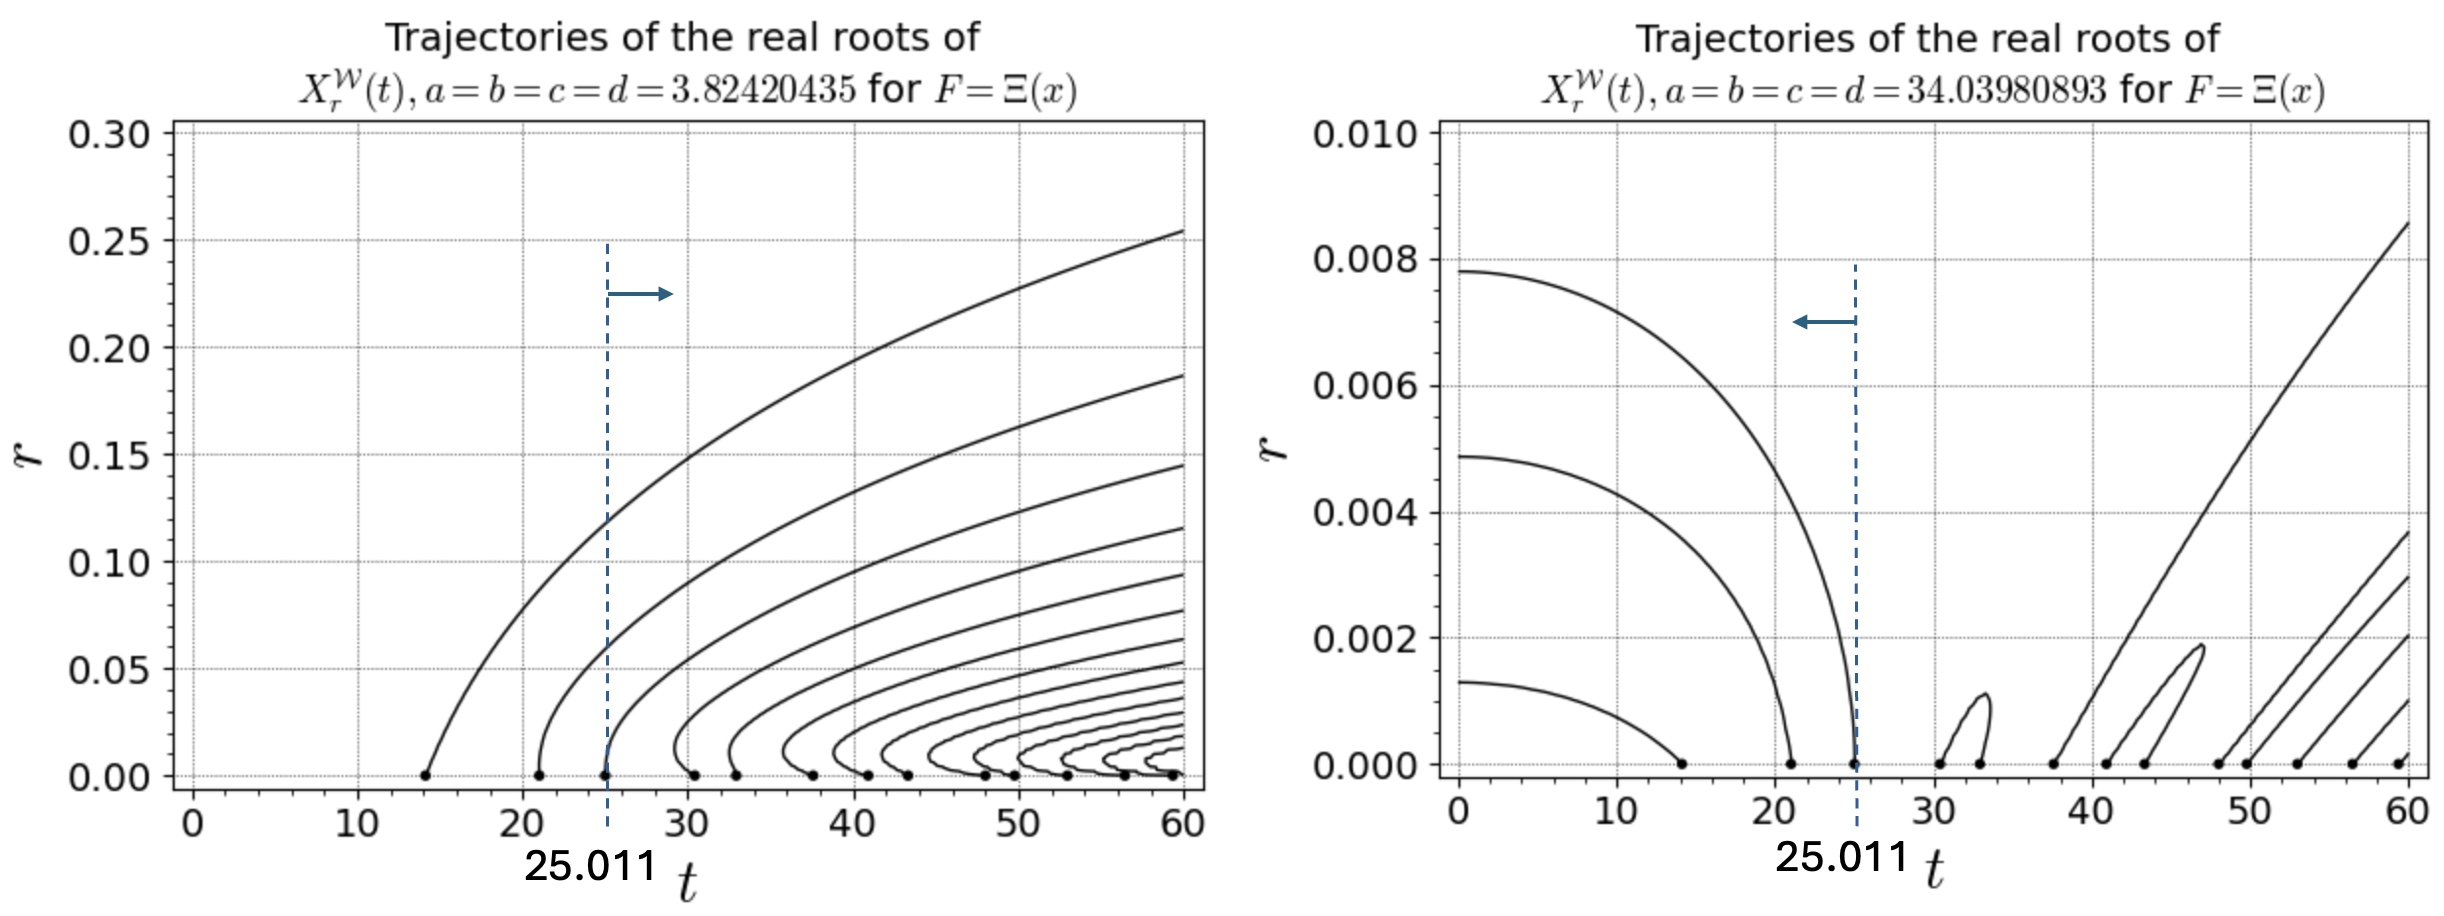
\includegraphics[width=0.9\linewidth]{WilsonCurveDouble.jpg}
  \caption{We show the two solutions for $a$ for the third zero where $\frac{\mathrm{d}}{\mathrm{d} r} z_3(0) = 0$. At the lower solution (left graph) we see the trajectories all being bent to the right, whereas for the higher solution (right graph) we see the trajectories being bent to the left and travelling again all the way back to the $r$-axis.}
  \label{fig:WilsonCurved}
\end{figure}

\small{
\begin{table}[H]
  \begin{center}
    \caption{Summary of our observations about the type B families when parameter $a$ is steadily increased. The hyperbolicity-effect no longer exists in any of the 4 families.}
    \label{tab:summary type B}
    \begin{tabular}{|l|l|c|c|} 
      \hline
       & & &\\
      Polynomial family & Parameters & \multicolumn{1}{|p{4cm}|}{\centering Does the flow start to \\increasingly resemble \\ the Pólya-DeBruijn flow?} & \multicolumn{1}{|p{3cm}|}{\centering Do all trajectories \\ eventually land \\ on the $r$-axis?} \\
      \hline
       & & &\\
      Meixner-Pollaczek &$(a,\pi/2)$ &Yes & No \\
      Continuous Hahn &$(a,a,a,a)$ & Yes & No \\
      Continuous Dual Hahn &$(a,a,a)$ & No & Yes \\ 
      Wilson &$(a,a,a,a)$ & No &Yes \\ 
       \hline
    \end{tabular}
  \end{center}
\end{table}
}

\section{Concluding remark}\label{concremarks}
 
In chapter 7 "Final remarks" of \cite{rom}, Romik makes the observation that:
\begin{quotation}
\textit{One rather striking fact is that the four different series expansions} (i.e. Pólya-De Bruijn, Hermite, Meixner Pollaczek, Continuous Hahn) \textit{we have considered for the Riemann $\Xi$ function, exhibit remarkably similar structural similarities: namely, in all four expansions the coefficients appear with alternating signs (and their asymptotics can be understood to a good level of accuracy, as our analysis shows). It is intriguing to wonder about the significance of this structural property of $\Xi(t)$. Can this information be exploited somehow to derive information about the location of the zeros of $\Xi(t)$? By way of comparison, one can consider “toy” expansions of the above forms involving more elementary coefficient sequences.}
\end{quotation}

He then shows the (trivial) reality of the zeros for all families, except for the Continuous Hahn polynomials. This raises the question whether anything could be said about the reality of the zeros of the $g_n$ polynomial expansion (i.e. the Continuous Hahn polynomials with parameters $\frac34, \frac34, \frac34, \frac34$). We found that after a slight change of parameters, it becomes quite easy to show that all zeros of the alternating generating function of the Continuous Hahn polynomial are real and regularly spaced for all $0 < r < 1$. We start from equation 9.4.11 in \cite{koe} and have:
\begin{align}
\sum_{n=0}^\infty (-1)^n\, \frac{(2)_{2n}}{\left(\frac32\right)_{2n}}\frac{ r^{2n}}{(2n)!}p_{2n}^{\left(\frac12,1,\frac12,1\right)}(t) &\verifiedeq \frac12\,\left(\frac{{}_2F_1\left(\left[1,\frac12-it\right],\left[1\right], -\frac{4r}{(1-r)^2}\right)}{(1-r)^2}+\frac{{}_2F_1\left(\left[1,\frac12-it\right],\left[1\right], \frac{4r}{(1+r)^2}\right)}{(1+r)^2} \right) \\
 & \verifiedeq \frac12\, \left(\frac{1}{\left(1-r \right)^{2}}\,\left(\left(\dfrac{r+1}{r -1}\right)^{2}\right)^{-\frac{1}{2}+it}+\frac{1}{{\left(1+r \right)^{2}}}\,\left(\left(\dfrac{r -1}{r+1}\right)^{2}\right)^{-\frac{1}{2}+it}\right) \notag
\end{align}
where the last equation has only real zeros (see table \ref{tab:tablezeros}).

Similarly we have for the Generalised Laguerre Polynomials the 'toy' generating function (note, we are using the traditional Laguerre polynomials here, not the 'even' version which we used for the flow-plots):
\begin{align}
\sum_{n=0}^\infty (-1)^n\,r^{2n} \,L_{2n}^{\left(a\right)}(t) \verifiedeq \frac12\,\left(\frac{1}{(1-ix)^{a+1}}\,\displaystyle \exp\left(\frac{-itx}{1-ix}\right)+\frac{1}{(1+ix)^{a+1}}\, \exp\left(\frac{itx}{1+ix}\right)\right)
\end{align}
which again only has real zeros that are well controlled (see table \ref{tab:tablezeros}).

This results in the list of "toy" expansions and the closed forms for their $n-$th zero (all real and simple):
{\footnotesize
\begin{table}[H]
  \begin{center}
    \caption{"Toy" expansions and the reality of their zeros}
    \label{tab:tablezeros}
    \begin{tabular}{|l|l|l|} 
      \hline
      Polynomial & Toy expansion for $0 < r < 1$ & Formula for the $n$-th zero, $ n \in \mathbb{Z}, r \in \mathbb{R}, |r| < 1$\\
      \hline
      & & \\
      "Polya De Bruijn" & $\displaystyle \sum_{n=0}^\infty (-1)^n\, \frac{ r^{2n}}{(2n)!}\,t^{2n}$  &$\displaystyle z_n(r) \verifiedeq \dfrac{\pi  \left(n-\frac12\right)}{r}$ \\       
      Hermite & $\displaystyle \sum_{n=0}^\infty (-1)^n\, \frac{ r^{2n}}{(2n)!}\, H_{2n}\left(t\right)$  &$\displaystyle z_n(r) \verifiedeq \dfrac{\pi  \left(n-\frac12\right)}{2r}$ \\
      General. Laguerre & $\displaystyle \sum_{n=0}^\infty (-1)^n\,r^{2n} \,L_{2n}^{\left(\alpha\right)}(t)$ & $\displaystyle z_n(r,\alpha) \verifiedeq i\,\frac{r^2+1}{2r}\,\left(\alpha\log\left(\frac{1-ir}{1+ir}\right)+\log\left(\frac{r+i}{r-i}\right)-2\pi i n\right)$ \\ 
      Meixner Pollaczek & $\displaystyle \sum_{n=0}^\infty (-1)^n\, r^{2n}\, P_{2n}^{\left(\lambda\right)}\left(t; \frac{\pi}{2}\right)$ &  $\displaystyle z_n(r) \verifiedeq \dfrac{\pi  \left(n-\frac12\right)}{\mathrm{log}\! \left(\dfrac{1+r}{1-r}\right)}$ \\
      Continuous Hahn & $\displaystyle \sum_{n=0}^\infty (-1)^n\, \frac{2n+1}{\left(\frac32\right)_{2n}}\,r^{2n}\,p_{2n}\left(t;\frac12,1,\frac12,1\right)$  & $\displaystyle z_n(r) \verifiedeq \dfrac{\pi  \left(n-\frac12\right)}{\mathrm{log}\! \left(\dfrac{r +1}{r-1}\right)-\mathrm{log}\! \left(\dfrac{r-1}{r+1}\right)}$\\
       & & \\
      \hline
    \end{tabular}
  \end{center}
\end{table}}

\pagebreak
\begin{thebibliography}{} 
\bibitem{rom}
Romik, D. \emph{Orthogonal polynomial expansions for the Riemann xi function in the Hermite, Meixner-Pollaczek, and continuous Hahn bases.}, Acta Arithmetica 200 (2021), 259-329.
Note: this paper exists in two different versions with different titles. See this page: https://www.math.ucdavis.edu/~romik/riemannxi/ for additional information and related resources. \\
\bibitem{pol}
D. H. J. Polymath, \emph{Effective approximation of heat flow evolution of the Riemann $\xi$ function, and a new upper bound for the de Bruijn-Newman constant}, Polymath 15 project, https://arxiv.org/abs/1904.12438.\\
\bibitem{arb}
Johansson, F. et al, \emph{FLINT/ARB - a C library for arbitrary-precision ball arithmetic}, https://flintlib.org.\\
\bibitem{map}
Maplesoft, \emph{Mathematics-based software solutions}, https://www.maplesoft.com.\\
\bibitem{koe}
Roelof Koekoek, Peter A. Lesky, René F. Swarttouw, \emph{Hypergeometric Orthogonal Polynomials and Their q-Analogues}, Springer, 2010, DOI 10.1007/978-3-642-05014-5\\
\bibitem{koesup}
Tom H. Koornwinder, \emph{Additions to the formula lists in “Hypergeometric orthogonal polynomials and their q-analogues” by Koekoek, Lesky and Swarttouw}, May 23, 2024, https://staff.fnwi.uva.nl/t.h.koornwinder/art/informal/KLSadd.pdf\\
\bibitem{rot}
B. Rodgers and T. Tao. \emph{The De Bruijn-Newman constant is non-negative.}, ArXiv e-prints, 2018. https://arxiv.org/abs/ 1801.05914\\
\bibitem{dob}
Dobner, A, \emph{A proof of Newman’s Conjecture for the extended Selberg class}, Acta Arithmetica 201 (2021), https://arxiv.org/abs/2005.05142\\
\bibitem{pla}
Platt, D., Trudgian, T., \emph{The Riemann hypothesis is true up to $3\,10^{12}$}, Bulletin of the London Mathematical Society, Volume 53, Issue 3, Pages: 643-962, June 2021\\
\bibitem{genoverview}
Hari Mohan Srivastava, \emph{Some Families of Generating Functions Associated with Orthogonal Polynomials and Other Higher Transcendental Functions}, MDPI, Mathematics 2022, 10(20), 3730; https://doi.org/10.3390/math10203730\\
\bibitem{meipolgen}
Wolter Groenevelt, Erik Koelink, Hjalmar Rosengren, \emph{Continuous Hahn functions as Clebsch-Gordan coefficients}, February 20, 2003, https://arxiv.org/abs/math/0302251v1\\
\bibitem{connex}
Michael A. Baeder, Howard S. Cohl, Hans Volkmer, \emph{Generalizations of generating functions for higher continuous hypergeometric orthogonal polynomials in the Askey scheme}, Journal of Mathematical Analysis and Applications, Elsevier, Volume 427, Issue 1, 1 July 2015, Pages 377-398\\
\bibitem{git} 
Dolph Dwars, Kalpesh Muchhal, \emph{GitHub environment with all code, data and graphs of this project}, https://github.com/km-git-acc/riemann-poly-expansions
\end{thebibliography}{} 

\appendix
\appendixpage
\renewcommand{\theequation}{A.\arabic{equation}}
\setcounter{equation}{0}
\section{Equations used for computing the Poisson Flows}\label{eqsused}
\begin{small}
\noindent\fbox{\begin{minipage}{\textwidth}
\begin{align}
\textbf{Legend:}& \notag \\
M_n(...) &\verifiedeq \text{the closed form of the orthogonality relation when $n=m$, see equation (\ref{ortrel})}. \notag \\
w_x(...) &\verifiedeq \text{the weight function, see equation (\ref{ortrel})}. \notag\\
g_n(...) &\verifiedeq \text{Factor before the hypergeom of the polynomial, see equation (\ref{deffn})}\notag \\
f_n(...) &\verifiedeq \bigg(g_n(...)\bigg)^2 / \,M_n(...)  \text{, see equation (\ref{deffn})}\notag \\
X_r^{\phi}(t;...)\left[F(t)\right] &\verifiedeq \text{the flow for polynomial family $\phi$.} \notag\\
\gamma_n(...) &\verifiedeq \text{coefficients of the expansion of the flow.} \notag \\
F(x) &\verifiedeq \text{the selected function to be expanded.} \notag  \\
-n(...)\,y(t) &\verifiedeq \text{the ODE or DDE for $y(t)=$ the polynomial under study.} \notag \\
\frac{\mathrm{d}}{\mathrm{d} r}z_k(r) &\verifiedeq \text{the first derivative of the $k$-th zero at "time" $r$ in the flow.} \notag \\
 \sum_{j \ne k}^{'} \frac{1}{z_k-z_j} &\verifiedeq \left(\sum_{j =1}^{k-1} \left(\frac{1}{z_k-z_j}\right)+\left(\frac{1}{z_k+z_j}\right)\right) +\left(\sum_{j = k+1}^{\infty} \left(\frac{1}{z_k-z_j}\right)+\left(\frac{1}{z_k+z_j}\right)\right)+\left(\frac{1}{2\,z_k} \right) \notag  \\
  \sum_{j \ne k}^{'} \frac{1}{2\pi k-2\pi j} &\verifiedeq -\frac{1}{2\pi k} \quad \text{for } F=\Xi_i \text{ at } r=0 \notag \\
\prod_{j \ne k}^{'} \frac{z_k+c-z_j}{z_k-z_j} &\verifiedeq c\,\left(\prod_{j =1}^{k-1} \left(1+\frac{c}{z_k-z_j}\right)\,\left(1+\frac{c}{z_k+z_j}\right)\right)\,\left(\prod_{j = k+1}^{\infty} \left(1+\frac{c}{z_k-z_j}\right)\,\left(1+\frac{c}{z_k+z_j}\right)\right)\,\left(1+\frac{c}{2\,z_k} \right) \notag \\
ZP(k,c) &\verifiedeq \prod_{j \ne k}^{'} \left(1-\frac{c}{2\pi k-2\pi j}\right)=2\,k\,\pi\,c^4\,(-1)^k\,\frac{\sin\left(\pi\,k+\dfrac{c}{2}\right)}{\pi\,k+\dfrac{c}{2}} \quad \text{for } F=\Xi_i \text{ at } r=0  \notag \\
  c &\verifiedeq \pm \,i \text{ or } \pm 1 \notag
\end{align}
\end{minipage}}

\pagebreak
\noindent\fbox{\begin{minipage}{\textwidth}
\begin{align}
  \textbf{Poisson}&\textbf{ Flow for the Hermite polynomials} \notag \\ \notag \\
  H_{2n}(x) &\defeq g_{2n} \,{}_1F_1\left(-n, \frac12,x^2\right)\\
  g_n &\verifiedeq i^n\,\frac{2^n\,\Gamma\left(\frac{n+1}{2}\right)}{\sqrt{\pi}} \\
  M_n &\defeq \sqrt{\pi}\,2^n\,n!\\
  w_x &\defeq \mathrm{e}^{-x^2}\\
  f_n &\verifiedeq (-1)^n\,\frac{2\,\Gamma\left(\frac{n}{2}+\frac12\right)}{\pi\,\Gamma(\frac{n}{2}+1)} \\
  -n\,y(x) &\verifiedeq \frac12\,y''(x)-x\,y'(x) \\
  X^\mathcal{H}_r(t)\left[F(t)\right] &\verifiedeq \sum_{n=0}^\infty \gamma_{2n}\,{}_1F_1\left(-n, \frac12,t^2\right)\,\exp(-2nr) = \Xi_{\tfrac{\exp(-r)^2-1}{4}} (\exp(-r)\,t) \\ 
  \gamma_n &\verifiedeq f_n\,\int_{0}^{\infty} F(x)\,w_x\,{}_1F_1\left(-\frac{n}{2}, \frac12,x^2\right)\,\mathrm{d}x \\
  \sum_{n=0}^\infty \gamma_n &\verifiedeq F(0) \\
\frac{\mathrm{d}}{\mathrm{d} r} z_k(r)&\verifiedeq-\,\sum_{j \ne k}^{'} \frac{1}{z_k(r)-z_j(r)} + z_k(r)\\
\frac{\mathrm{d}}{\mathrm{d} r} z_k(0)&\verifiedeq \frac{1}{2\,k\,\pi} + 2\,k\,\pi \quad \text{when } F=\Xi_i
\end{align}
\end{minipage}}
\begin{figure}[H]
  \noindent
  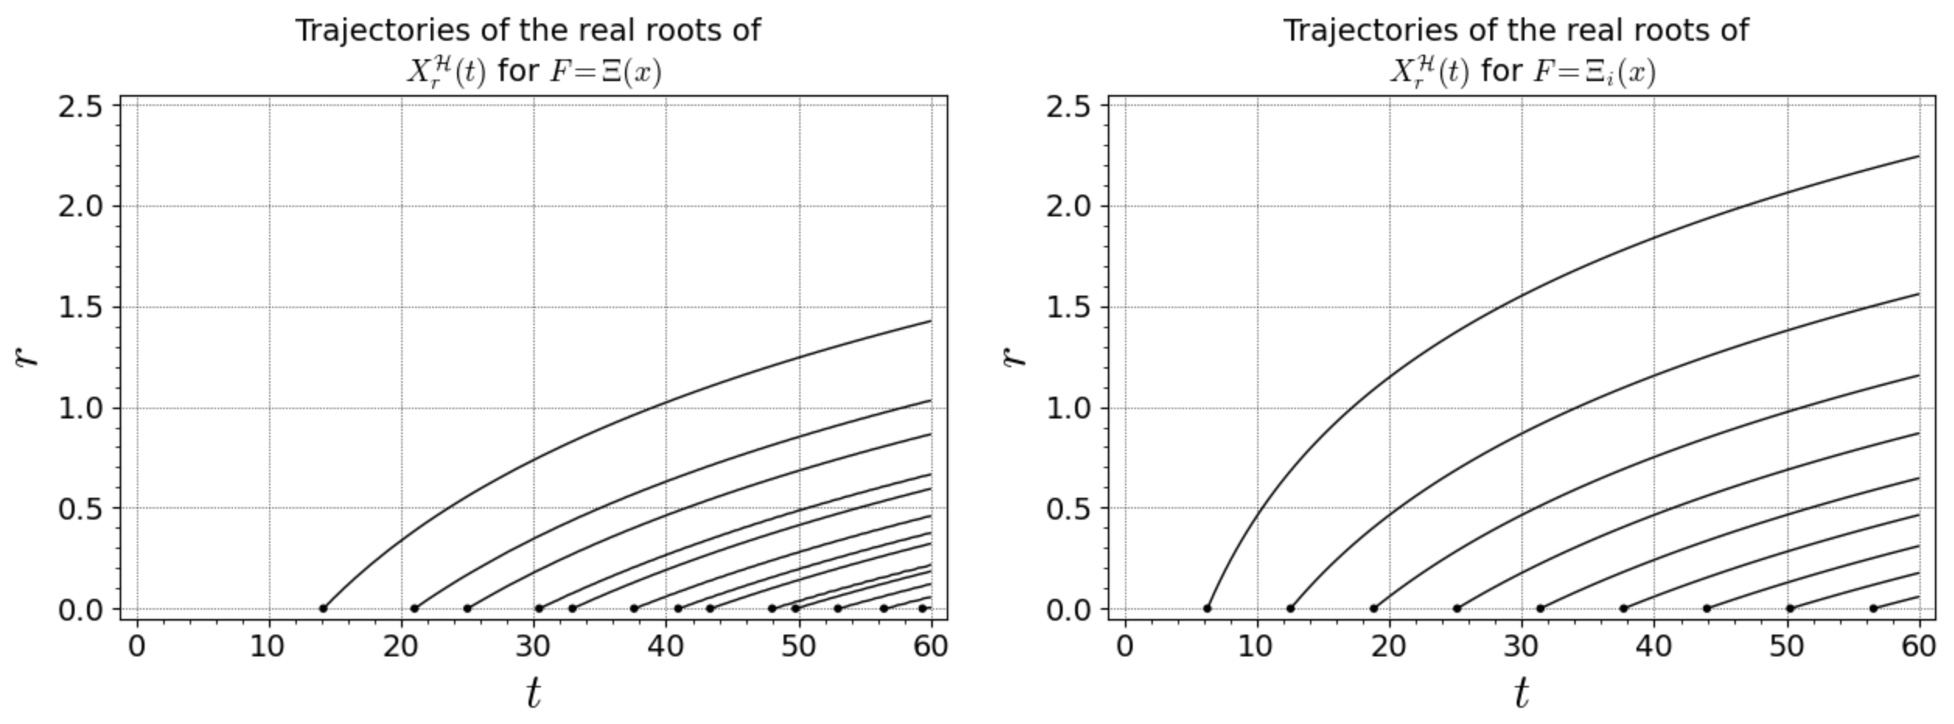
\includegraphics[width=1\linewidth]{HermiteFlowdouble.jpg}
  \caption{The graphs show the Poisson flows of the Hermite polynomial expansions for $\Xi(t)$ (left) and $\Xi_i(t)$ (right). We know these flows are the transformation of the Pólya de Bruijn flow, i.e.: $X^\mathcal{H}_r(t) \verifiedeq \Xi_{\frac{\exp(-2r)-1}{4}} (\exp(-r)\,t)$. The mapping $\exp(-r), r > 0$ can only cover the domain $-0.25 \le \lambda \le 0$, so we don't expect collisions to show up in the right hand graph (since all collisions in the flow $\Xi_{\lambda\,i}$ reside at increasingly negative $\lambda \ll -0.25)$. There are collisions between $-0.25..0$ for $\Xi_{\lambda}$ at higher $t$, so these will show up at some point in the left hand graph (see Figure \ref{fig:flowLcoll} for an example).}
  \label{fig:flowH1}
\end{figure}

\pagebreak
\end{small}
\begin{normalsize}
Computations with the expansion of $F$ into the traditional Laguerre polynomials revealed that the coefficients behaved quite randomly. We therefore decided to opt for an orthogonal system of even Laguerre functions that we denote $ \hat{L}^{\alpha}_n(x)$. This provides a much better fit with the even function $F$. 

\end{normalsize}
\begin{small}
\noindent\fbox{\begin{minipage}{\textwidth}
\begin{align}
  \textbf{Poisson}&\textbf{ Flow for the Generalised even Laguerre polynomials} \notag \\
  \hat{L}^{\alpha}_n(x) &\defeq g_n(\alpha)\, {}_1F_1(-n, \alpha+1,x^2) \\
  g_n(\alpha) &\verifiedeq \frac{(\alpha+1)_n}{n!} \\
  M_n(\alpha) &\defeq \frac{\Gamma(\alpha+1+n)}{2\,n!} \\
  w_x(\alpha) &\defeq \mathrm{e}^{-x^2}\,x^{2\alpha+1}\\
  f_n(\alpha) &\verifiedeq \frac{2\,\Gamma\left(n+\alpha+1\right)}{\Gamma(\alpha+1)^2\,n!} \\
  -n\,y(x) &\verifiedeq \frac14\,y''(x)+\left(\frac{2\alpha+1}{4x}-\frac{x}{2}\right)\,y'(x) \label{lagPDE}\\
  X^{\mathcal{L}}_r(t;\alpha)\left[F(t)\right] &\verifiedeq \sum_{n=0}^\infty \gamma_n(\alpha)\,{}_1F_1\left(-n, \alpha+1,t^2\right)\,\exp(-2nr) \\ 
  \gamma_n(\alpha) &\verifiedeq f_n(\alpha)\int_{0^+}^{\infty} F(x)\,w_x(\alpha)\,{}_1F_1\left(-n, \alpha+1,x^2\right)\,\mathrm{d}x \label{lagflow}\\
  \sum_{n=0}^\infty \gamma_n(\alpha) &\verifiedeq F(0) \\
  \frac{\mathrm{d}}{\mathrm{d} r} z_k(r)&\verifiedeq-\sum_{j \ne k}^{'} \frac{1}{z_k(r)-z_j(r)} -\frac{\alpha+\frac12}{z_k(r)}+z_k(r) \label{zerodiff}\\
  \frac{\mathrm{d}}{\mathrm{d} r} z_k(0)&\verifiedeq \frac{1-\alpha-\frac12}{2\,k\,\pi}+2\,k\,\pi \quad \text{when } F=\Xi_i \label{zeroclosed}
\end{align}
\end{minipage}}
\begin{figure}[H]
  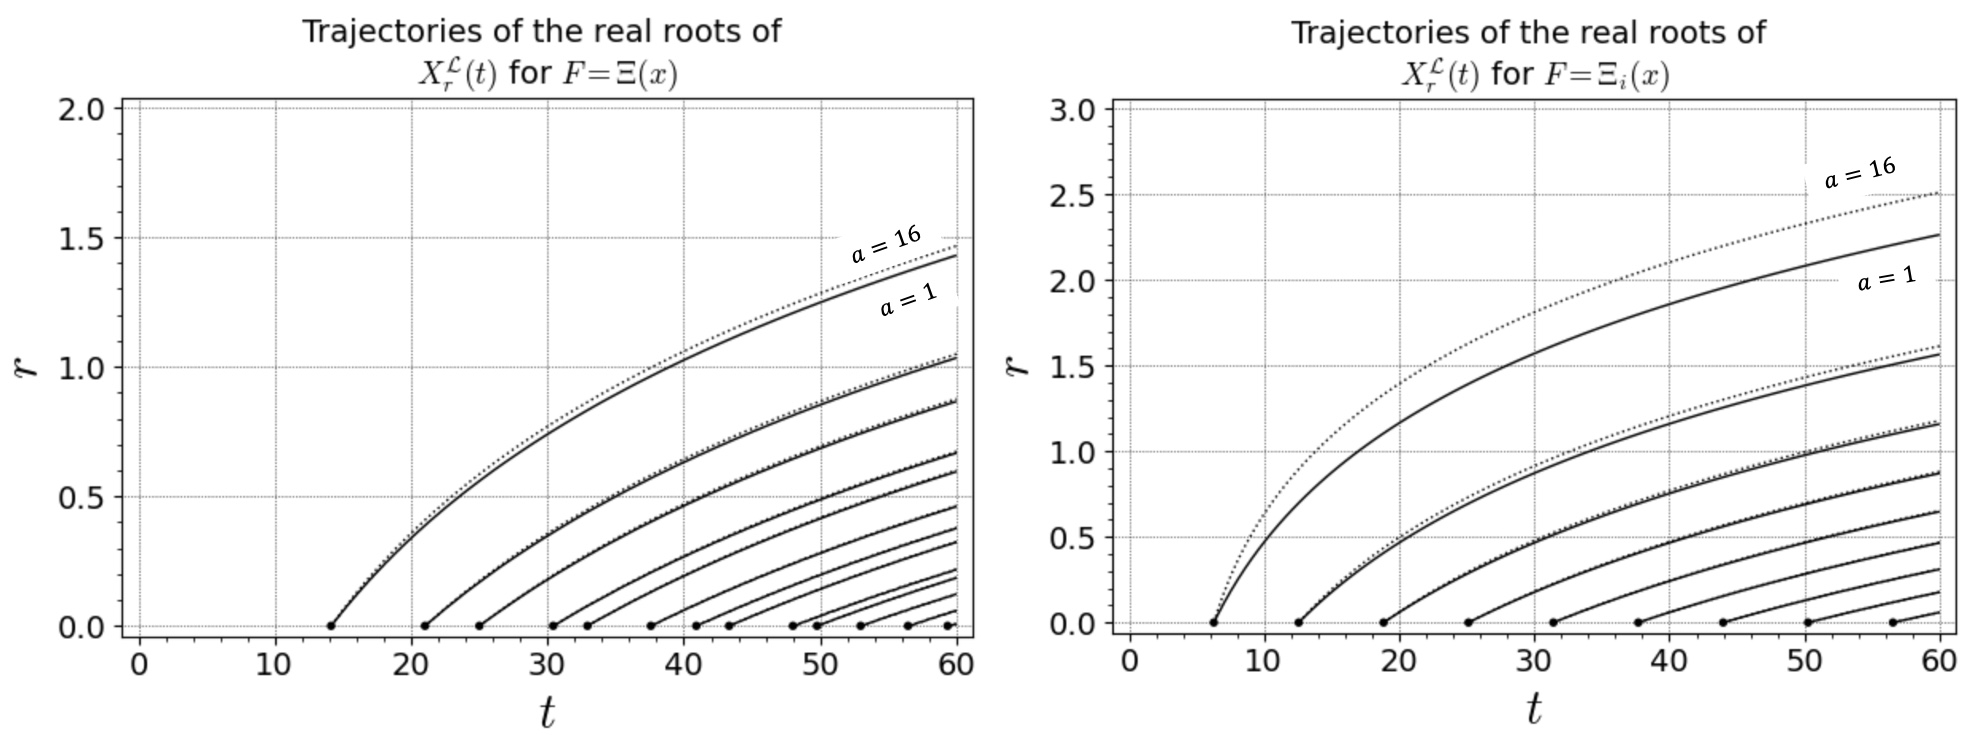
\includegraphics[width=1\linewidth]{LaguerreFlowdouble.jpg}
  \caption{The graphs show the Poisson flows of the Generalised Laguerre polynomial expansions for $\Xi(t)$ (left) and $\Xi_i(t)$ (right). We show the flow for the parameters $\alpha = 1$ and $\alpha = 16$. A change of parameter $\alpha$ induces a rotation around $r=0$. When $\alpha$ decreases the rotation is clockwise, when $\alpha0$ increases it turns counter-clockwise. Collisions can occur when $r$ is increased (see Figure \ref{fig:flowLcoll} for an example).}
  \label{fig:flowL}
\end{figure}
\pagebreak
\noindent\fbox{\begin{minipage}{\textwidth}
\begin{align}
  \textbf{Poisson}&\textbf{ Flow for the Meixner Pollaczek polynomials with $\Phi = \frac{\pi}{2}$} \notag \\
  P_n^{(\lambda)}\left(x; \frac{\pi}{2}\right) &\defeq g_n(\lambda)\,{}_2F_1\left([-n, \lambda+i\,x],[2\lambda],2\right)\\
  g_n(\lambda) &\verifiedeq i^n\,\frac{(2\lambda)_n}{n!}\\
  M_n(\lambda) &\defeq \frac{2\,\pi\,\Gamma(n+2\lambda)}{2^{2\lambda}\,n!} \\
  w_x(\lambda) &\defeq \Gamma(\lambda+ix)\,\Gamma(\lambda-ix) \\
  f_n(\lambda) &\verifiedeq \frac{4^\lambda\,\Gamma(n+2\lambda)}{2\,\pi\,\Gamma(2\lambda)^2\,\Gamma(n+1)} \\
  -n\,y(x) &\verifiedeq -\frac12\,(\lambda-ix)\,y(x+i)+\lambda\,y(x)-\frac12\,(\lambda+ix)\,y(x-i) \\
  X^\mathcal{MP}_r(t;\lambda)\left[F(t)\right] &\verifiedeq \sum_{n=0}^\infty \gamma_{2n}(\lambda)\,{}_2F_1\left([-2n, \lambda+it],[2\lambda],2\right)\,\exp\left(-2nr\right) \\ 
  \gamma_n(\lambda) &\verifiedeq f_n(\lambda)\,\int_{-\infty}^{\infty} F(x)\,w_x(\lambda)\,{}_2F_1\left([-n, \lambda+ix],[2\lambda],2\right)\,\mathrm{d}x \\
  \sum_{n=0}^\infty \gamma_n(\lambda) &\verifiedeq F(i\lambda) \\
  \frac{\mathrm{d}}{\mathrm{d} r} z_k(r)&\verifiedeq  \left(\frac{\lambda-i\,z_k(r)}{2}\right)\,\prod_{j \ne k}^{'} \left(1+\frac{i}{z_k(r)-z_j(r)}\right)+\left(\frac{\lambda+i\,z_k(r)}{2}\right)\,\prod_{j \ne k}^{'} \left(1-\frac{i}{z_k(r)-z_j(r)}\right) \label{zerodiffmp} \\
  \frac{\mathrm{d}}{\mathrm{d} r} z_k(0)&\verifiedeq \left(\frac{\lambda}{2}-k\,\pi\,i\right)\,ZP(k,i)+\left(\frac{\lambda}{2}+k\,\pi\,i\right)\,ZP(k,-i)\quad \text{when } F=\Xi_i 
\end{align}
\end{minipage}}
\begin{figure}[H]
  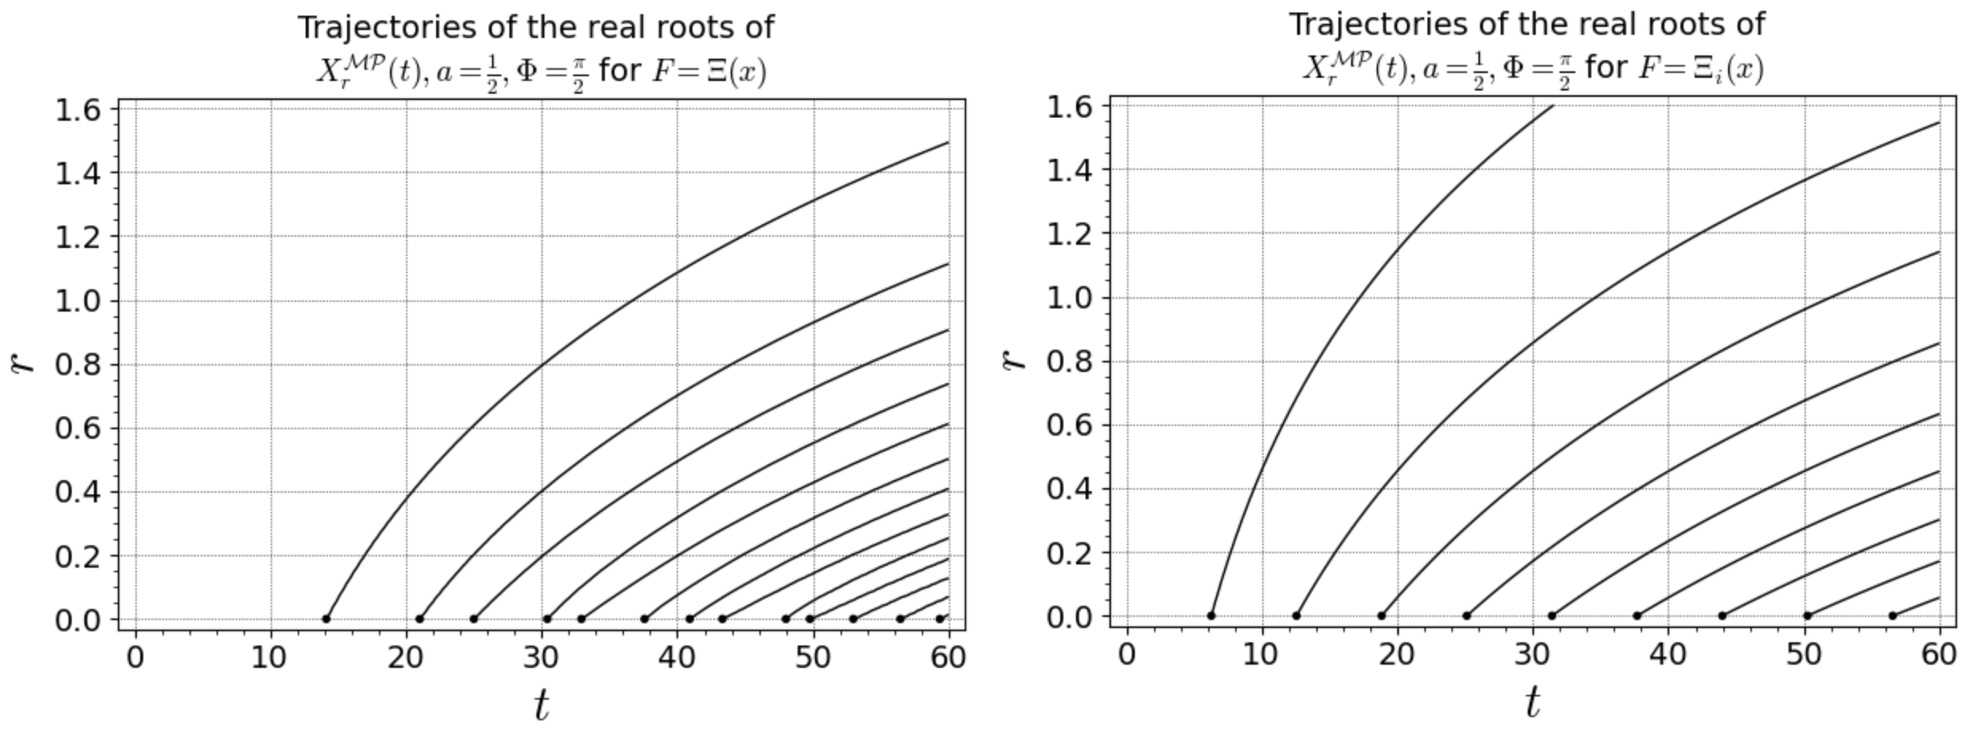
\includegraphics[width=1\linewidth]{MeixPollFlowdouble.jpg}
  \caption{The graphs show the Poisson flows of the Meixner-Pollaczek polynomial expansions for $\Xi(t)$ (left) and $\Xi_i(t)$ (right) for a fixed set of parameters.  When $r$ increases the flows seem to eventually line up vertically into an arithmetic progression (for this specific value of $a$).}
  \label{fig:flowMP}
\end{figure}
\pagebreak
\noindent\fbox{\begin{minipage}{\textwidth}
\begin{align}
  \textbf{Poisson}&\textbf{ Flow for the Continuous Dual Hahn polynomials} \notag \\
  S_n(x^2;a,b,c) &\defeq g_n(a,b,c)\, {}_3F_2([-n,a+ix, a- ix], [a+b, a+c], 1) \\
  g_n(a,b,c) &\verifiedeq (a+b)_n\,(a+c)_n  \\
  M_n(a,b,c) &\defeq 2\pi\,n!\,\Gamma(n+a+b)\,\Gamma(n+a+c)\,\Gamma(n+b+c) \\
  w_x(a,b,c) &\defeq \left|\frac{\Gamma(a+ix)\,\Gamma(b+ix)\,\Gamma(c+ix)}{\Gamma(2ix)}\right|^2 \\
  f_n(a,b,c) &\verifiedeq \frac{\Gamma(n+a+b)\,\Gamma(n+a+c)}{2\,\pi\,\Gamma(a+b)^2\,\Gamma(a+c)^2\,n!\,\Gamma(n+b+c)} \\
  -n\,y(x) &\verifiedeq -B(x)\,y(x+i)+\left(B(x)+D(x)\right)\,y(x)-D(x)\,y(x-i) \\
  B(x)&\verifiedeq\frac{(a-ix)\,(b-ix)\,(c-ix)}{2ix\,(2ix-1)} \\
  D(x)&\verifiedeq\frac{(a+ix)\,(b+ix)\,(c+ix)}{(2ix\,(2ix+1)} \\
  X^\mathcal{CDH}_r(t;a,b,c)\left[F(t)\right] &\verifiedeq \sum_{n=0}^\infty \gamma_n(a,b,c)\,{}_3F_2\left([-n, a+it, a-it],[a+b,a+c],1\right)\,\exp\left(-nr\right) \\ 
  \gamma_n(a,b,c) &\verifiedeq f_n(a,b,c)\,\int_{0}^{\infty} F(x)\,w_x(a,b,c)\,{}_3F_2\left([-n, a+ix, a-ix],[a+b,a+c],1\right)\,\mathrm{d}x \\
  \sum_{n=0}^\infty \gamma_n(a,b,c) &\verifiedeq F(\pm ia) \\
  \frac{\mathrm{d}}{\mathrm{d} r} z_k(r)&\verifiedeq B\big(Z_k(r)\big)\,\prod_{j \ne k}^{'} \left(1+\frac{i}{z_k(r)-z_j(r)}\right)+D\big(Z_k(r)\big)\,\prod_{j \ne k}^{'} \left(1-\frac{i}{z_k(r)-z_j(r)}\right) \label{zerodiffcdh}\\
  \frac{\mathrm{d}}{\mathrm{d} r} z_k(0)&\verifiedeq B\big(2\,k\,\pi\big)\,ZP(k,i)+D\big(2\,k\,\pi)\,ZP(k,-i)\quad \text{when } F=\Xi_i 
\end{align}
\end{minipage}}
\begin{figure}[H]
  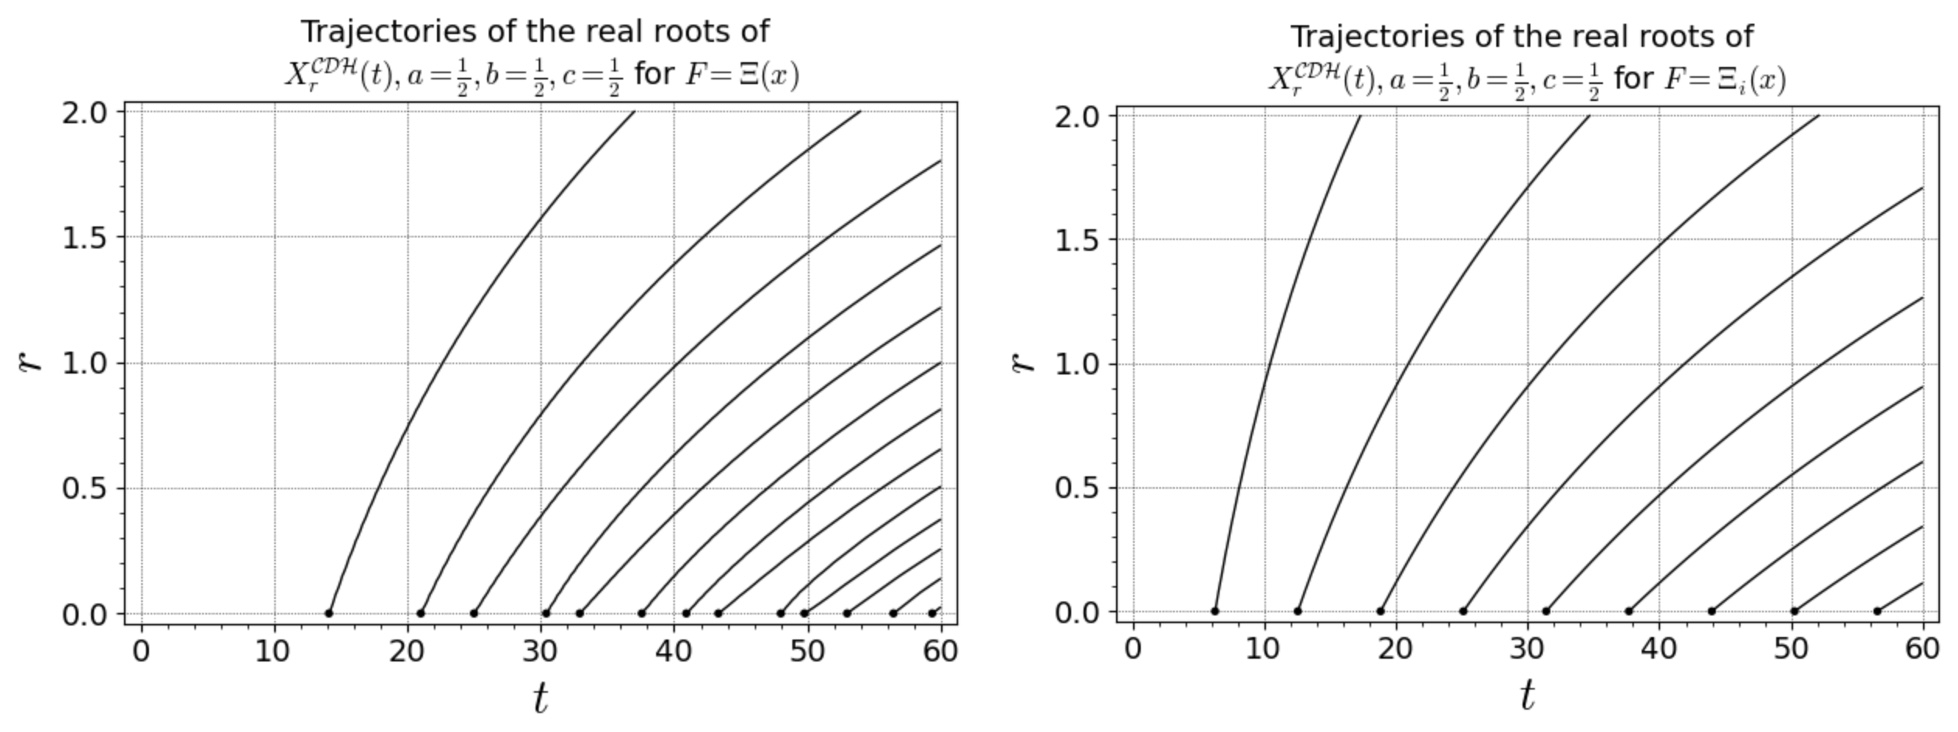
\includegraphics[width=1\linewidth]{ContDualHahnFlowdouble.jpg}
  \caption{The graphs show the Poisson flows of the Continuous Dual Hahn polynomial expansions for $\Xi(t)$ (left) and $\Xi_i(t)$ (right) for a fixed set of parameters. When $r$ increases the flows seem to eventually line up vertically into an arithmetic progression (for this specific value of $a,b,c$).}
  \label{fig:flowLCDH}
\end{figure}
\pagebreak
\noindent\fbox{\begin{minipage}{\textwidth}
\begin{align}
  \textbf{Poisson}&\textbf{ Flow for the Continuous Hahn polynomials} \notag \\
  \kappa_n &= n + a + b + c + d - 1 \\
  p_n(x;a,b,c,d) &\defeq g_n(a,b,c,d)\,{}_3F_2\left([-n, \kappa_n, a+ix],[a+c,a+d],1\right) \\
  g_n(a,b,c,d) &\verifiedeq i^n\,\frac{(a+c)_n\,(a+d)_n}{n!} \\
  M_n(a,b,c,d) &\defeq \frac{2\pi\,\Gamma(n+a+c)\,\Gamma(n+a+d)\,\Gamma(n+b+c)\,\Gamma(n+b+d)}{(n+\kappa_n)\,\Gamma(\kappa_n)\,n!} \\
  w_x(a,b,c,d) &\defeq \Gamma(a+ix)\,\Gamma(b+ix)\,\Gamma(c-ix),\Gamma(d-ix) \\
  f_n(a,b,c,d) &\verifiedeq \frac{\Gamma(n+a+c)\,\Gamma(n+a+d)\,\Gamma(\kappa_n)\,(n+\kappa_n)}{2\,\pi\,\Gamma(a+c)^2,\Gamma(a+d)^2\,\Gamma(n+1)\,\Gamma(n+b+c)\,\Gamma(n+b+d)} \\
 -n\,\kappa_n\,y(x) &\verifiedeq -B(x)\,y(x+i)+\left(B(x)+D(x)\right)\,y(x)-D(x)\,y(x-i) \\
  B(x)&\verifiedeq (c-ix)\,(d-ix) \\
  D(x)&\verifiedeq (a+ix)\,(b+ix) \\
  X^\mathcal{CH}_r(t;a,b,c,d)\left[F(t)\right] &\verifiedeq \sum_{n=0}^\infty \gamma_n(a,b,c,d)\,{}_3F_2\left([-n, \kappa_n, a+it],[a+c,a+d],1\right)\,\exp\left(-n\,\kappa_n\,r\right) \\ 
  \gamma_n(a,b,c,d) &\verifiedeq f_n(a,b,c,d)\,\int_{0}^{\infty} F(x)\,w_x(a,b,c,d) {}_3F_2\left([-n, \kappa_n, a+ix],[a+c,a+d],1\right)\,\mathrm{d}x \\
  \sum_{n=0}^\infty \gamma_n(a,b,c,d) &= F(ia) \\
  \frac{\mathrm{d}}{\mathrm{d} r} z_k(r)&\verifiedeq B\big(Z_k(r)\big)\,\prod_{j \ne k}^{'} \left(1+\frac{i}{z_k(r)-z_j(r)}\right)+D\big(Z_k(r)\big)\,\prod_{j \ne k}^{'} \left(1-\frac{i}{z_k(r)-z_j(r)}\right) \label{zerodiffch} \\
  \frac{\mathrm{d}}{\mathrm{d} r} z_k(0)&\verifiedeq B\big(2\,k\,\pi\big)\,ZP(k,i)+D\big(2\,k\,\pi)\,ZP(k,-i)\quad \text{when } F=\Xi_i 
\end{align}
\end{minipage}}
\begin{figure}[H]
  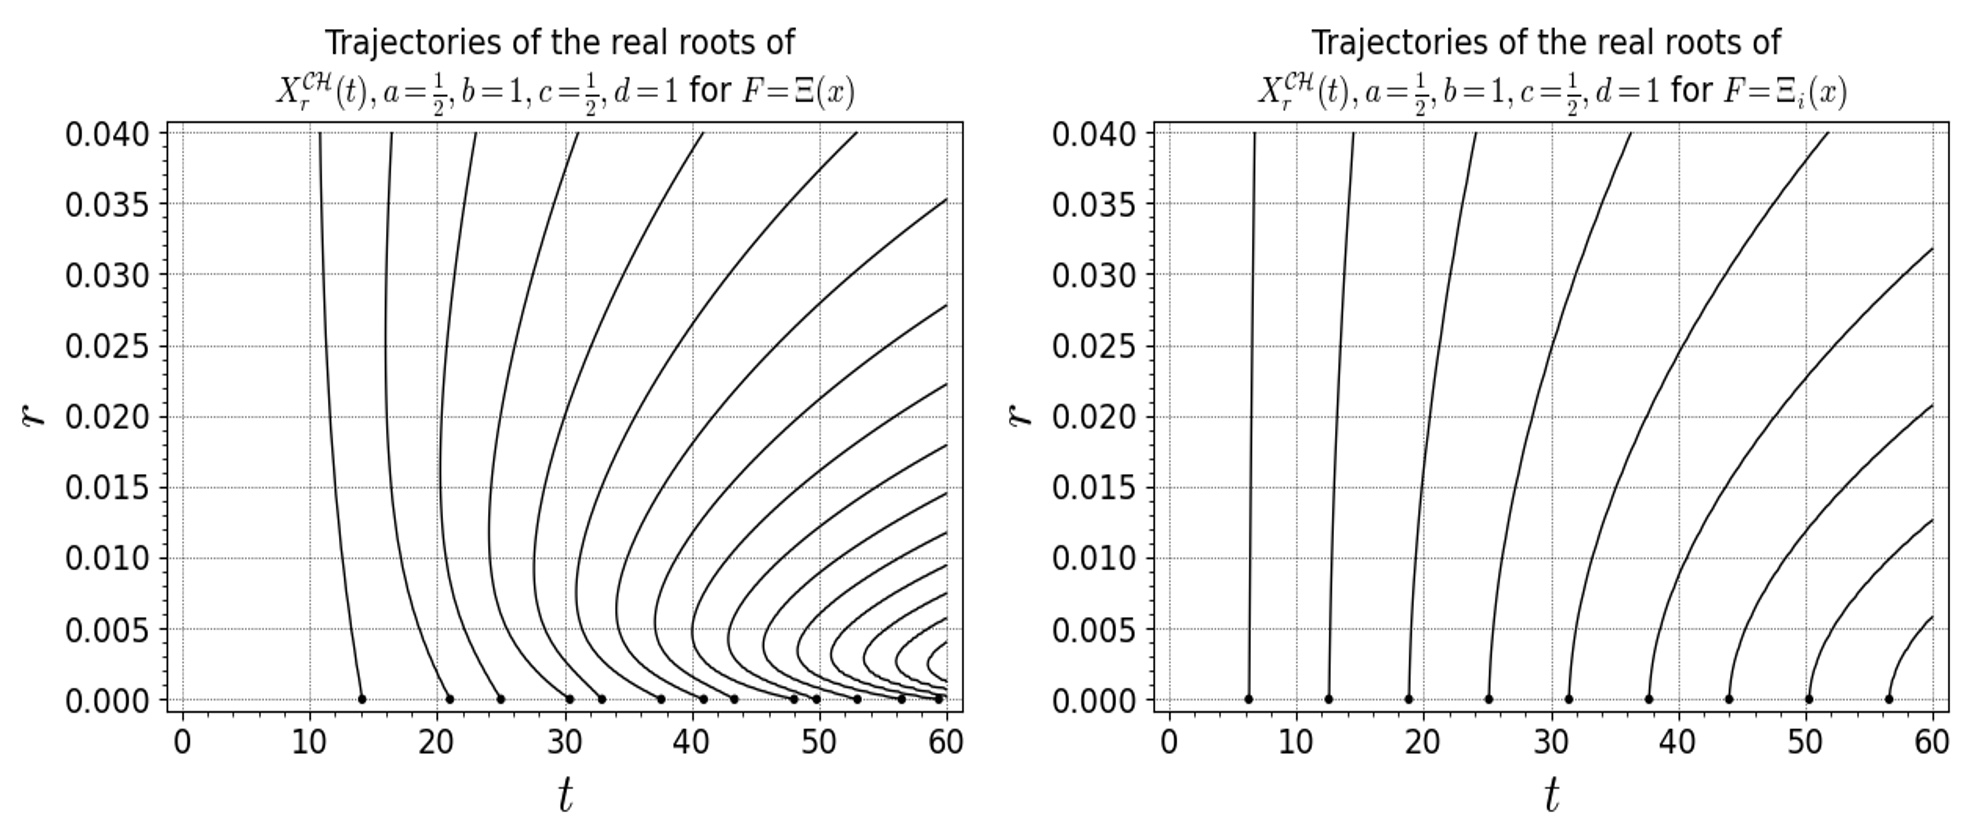
\includegraphics[width=1\linewidth]{ContHahnFlowdouble.jpeg}
  \caption{The graphs show the Poisson flows of the Continuous Hahn polynomial expansions for $\Xi(t)$ (left) and $\Xi_i(t)$ (right) for a fixed set of parameters. When $r$ increases the flows seem to eventually line up vertically into an arithmetic progression (for this specific value of $a,b,c,d$).}
  \label{fig:flowCH}
\end{figure}
\pagebreak
\noindent\fbox{\begin{minipage}{\textwidth}
\begin{align}
  \textbf{Poisson}&\textbf{ Flow for the Wilson polynomials} \notag \\  
  \kappa_n &\defeq n + a + b + c + d - 1 \\
  W_n(y^2;a,b,c,d) &\defeq  g_n(a,b,c,d) \, {}_4F_3([-n, \kappa_n,a+iy, a- iy], [a+b, a+c, a+d], 1) \\
  g_n(a,b,c,d) &\verifiedeq (a+b)_n\,(a+c)_n\,(a+d)_n \\
  M_n(a,b,c,d) &\defeq \frac{2\pi(\kappa_n)_nn!\Gamma(n+a+b)\Gamma(n+a+c)\Gamma(n+a+d)\Gamma(n+b+c)\Gamma(n+b+d)\Gamma(n+c+d)}{\Gamma(2n+a+b+c+d)}\\
  w_x(a,b,c,d) &\defeq \left|\frac{\Gamma(a+ix)\,\Gamma(b+ix)\,\Gamma(c+ix)\,\,\Gamma(d+ix)}{\Gamma(2ix)}\right|^2 \\
  f_n(a,b,c,d) &\verifiedeq \frac{(a+b)_n^2\,(a+c)_n^2\,(a+d)_n^2\,\Gamma(2n+a+b+c+d)}{2\pi\,(\kappa_n)_n\Gamma(n+a+b)\Gamma(n+a+c)\Gamma(n+a+d)n!\Gamma(n+b+c)\Gamma(n+b+d)\Gamma(n+c+d)}\\
  -n\,\kappa_n\,y(x) &\verifiedeq -B(x)\,y(x+i)+\left(B(x)+D(x)\right)\,y(x)-D(x)\,y(x-i)\label{wildde} \\ 
  B(x)&\verifiedeq \frac{(a-ix)\,(b-ix)\,(c-ix)\,(d-ix)}{2ix\,(2ix-1)} \\
  D(x)&\verifiedeq \frac{(a+ix)\,(b+ix)\,(c+ix)\,(d+ix)}{2ix\,(2ix+1)} \\
  X^\mathcal{W}_r(t;a,b,c,d)\left[F(t)\right] &\verifiedeq \sum_{n=0}^\infty \gamma_n(a,b,c,d)\,{}_4F_3\left(\left[-n, \kappa_n,a+it, a- it\right], \left[a+b, a+c, a+d\right], 1\right)\,\exp\left(-n\,\kappa_n\,r\right) \label{wilflow} \\
  \gamma_n(a,b,c,d) &\verifiedeq f_n(a,b,c,d)\int_{0}^{\infty} F(x)\,w_x(){}_4F_3\left(\left[-n, \kappa_n,a+ix, a- ix\right], \left[a+b, a+c, a+d\right], 1\right)\,\mathrm{d}x \\
  \sum_{n=0}^\infty \gamma_n(a,b,c,d) &\verifiedeq F(\pm ia) \\
  \frac{\mathrm{d}}{\mathrm{d} r} z_k(r)&\verifiedeq B\big(Z_k(r)\big)\,\prod_{j \ne k}^{'} \left(1+\frac{i}{z_k(r)-z_j(r)}\right)+D\big(Z_k(r)\big)\,\prod_{j \ne k}^{'} \left(1-\frac{i}{z_k(r)-z_j(r)}\right) \label{zerodiffw}\\
  \frac{\mathrm{d}}{\mathrm{d} r} z_k(0)&\verifiedeq B\big(2\,k\,\pi\big)\,ZP(k,i)+D\big(2\,k\,\pi)\,ZP(k,-i)\quad \text{when } F=\Xi_i 
\end{align}
\end{minipage}}
\begin{figure}[H]
  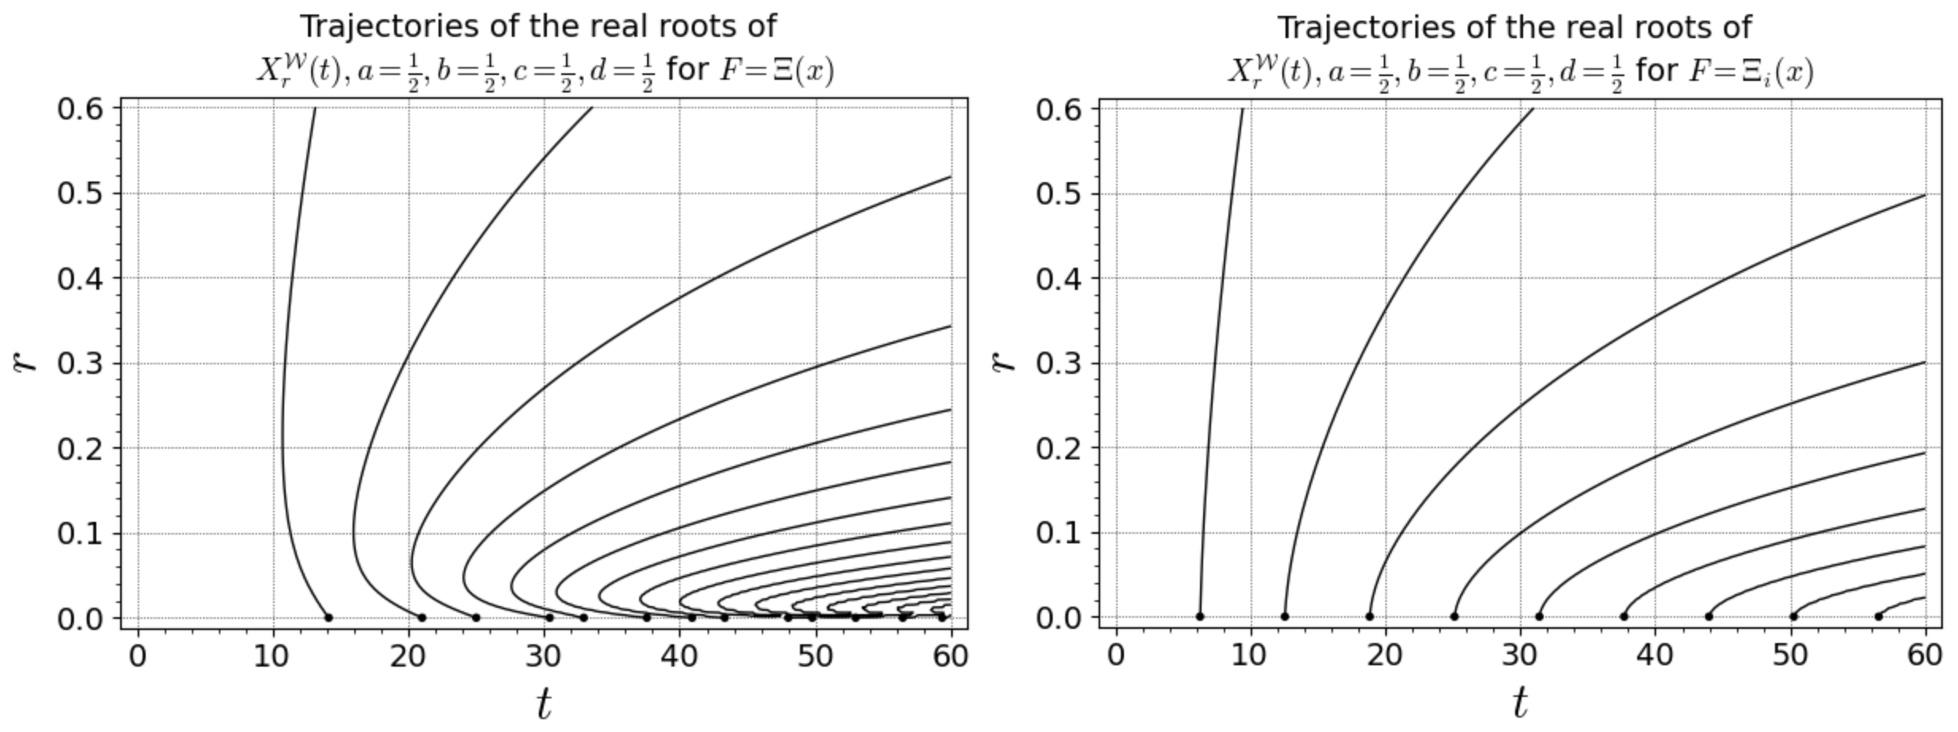
\includegraphics[width=1\linewidth]{WilsonFlowdouble.jpg}
  \caption{The graphs show the Poisson flows of the Wilson polynomial expansions for $\Xi(t)$ (left) and $\Xi_i(t)$ (right) for a fixed set of parameters. When $r$ increases the flows seem to eventually line up vertically into an arithmetic progression (for this specific value of $a,b,c,d$).}
  \label{fig:flowW2}
\end{figure}
\end{small}
\pagebreak

\renewcommand{\theequation}{B.\arabic{equation}}
\setcounter{equation}{0}
\section{A list of alternatives for the coefficients of various Riemann $\Xi-$ and $\Xi'-$function expansions}\label{specexpansions}

There is a limited set of orthogonal polynomial families whose generating functions can be directly associated with the kernel of the Fourier cosine transform of $\Xi(t)$ or the sine transform of $\Xi'(t)$ (see Table \ref{tab:tablefunc}). Such a connection arises from the closed form of the generating functions, which can be expressed using specific parameters and extended to a broader domain through an appropriate mapping.

Once this link is established, known relationships between different polynomial families can be utilized to progress within the Askey-scheme. In some cases, this transition is achieved through a straightforward equation involving a single parameter. However, when an additional parameter is required, a finite sum formula becomes necessary. The table below presents a streamlined version of our results for the expansions of $\Xi(t)$, displaying only the integral components of the simplified coefficients for easier comparison. The full expressions, including those for $\Xi'(t)/t$, along with detailed derivations, are provided in subsequent sections. 

These simplified expressions are particularly valuable for expediting computations and for analysing the asymptotics of the expansion's coefficients.

\begin{footnotesize}
\begin{table}[H]
  \begin{center}
    \caption{Simplified coefficients for specific parameter choices for expanding $\Xi(t)$}
    \label{tab:tablecoeff}
    \begin{tabular}{|l|l|l|} 
      Poisson Flow: & Expansion into orthogonal family: & Expansion coefficient:\\
      \hline
      $X^{\mathcal{H}}_r(t)\left[\Xi(t)\right]$ & $\displaystyle \sum_{n=0}^\infty H_{2n}(t)\,\gamma_{2n}\,r^{2n}$  &$\displaystyle\gamma_{2n}=\frac{i^{2n}}{2^{2n}\,(2n)!}\int_{-\infty}^{\infty} \Phi(x)\,x^{2n}\,\mathrm{e}^{-x^2/4}\,\mathrm{d}x$ \\
      $X^{\mathcal{L}}_r(t;-1/2)\left[\Xi(t)\right]$ & $\displaystyle \sum_{n=0}^\infty L^{-1/2}_n\left(t^2\right)\,\gamma_n\,r^n$  &$\displaystyle\gamma_n=\frac{n!}{(2n)!}\int_{-\infty}^{\infty} \Phi(x)\,x^{2n}\,\mathrm{e}^{-x^2/4}\mathrm{d}x$ \\
      $X^{\mathcal{L}}_r(t;\alpha)\left[\Xi(t)\right]$ & $\displaystyle \sum_{n=0}^\infty L^{\alpha}_n(t)\,\gamma_n\,r^n$  &$\displaystyle \gamma_n=\int_{-\infty}^{\infty} \Phi(x)\,\left(\frac{ix}{ix+1}\right)^n\,\left(\frac{1}{ix+1}\right)^{a+1}\,\mathrm{d}x $ \\
      $X^\mathcal{MP}_r(t;a)\left[\Xi(t)\right]$ & $\displaystyle \sum_{n=0}^\infty P_{2n}^{(a)}\left(t;\frac{\pi}{2}\right)\,\gamma_{2n},r^{2n}$  &$\displaystyle\gamma_{2n}=4^a\,i^{2n}\,\int_{-\infty}^{\infty} \Phi(x)\,T(x)^{2n}\,\frac{\textrm{e}^{a\,x}}{(\textrm{e}^x+1)^{2a}}\,\mathrm{d}x$ \\
      $X^\mathcal{CH}_r(t;a)\left[\Xi(t)\right]$ & $\displaystyle \sum_{n=0}^\infty p_{2n}\left(\frac{t}{2};\frac{a}{2},\frac{a+1}{2},\frac{a}{2},\frac{a+1}{2}\right) \gamma_{2n}\,r^{2n}$  &$\displaystyle\gamma_{2n}=\frac{2^{4n}\,4^a\,i^{2n}}{(2a+2n)_{2n}} \,\int_{-\infty}^{\infty} \Phi(x)\,T(x)^{2n}\,\frac{\textrm{e}^{a\,x}}{(\textrm{e}^{x}+1)^{2a}}\,\mathrm{d}x$ \\
      $X^\mathcal{CH}_r(t;a,b)\left[\Xi(t)\right]$ & $\displaystyle \sum_{n=0}^\infty\,p_{2n}\left(t;a,b,a,b\right)\, \gamma_{2n}\,r^{2n}$  &$\displaystyle\gamma_{2n}=\frac{2^{2n}\,4^a\,i^{2n}}{\left(2a+2b+2n-1\right)_{2n}} \,\int_{-\infty}^{\infty} \Phi(x)T(x)^{2n}\frac{\textrm{e}^{a\,x}}{(\textrm{e}^{x}+1)^{2a}}h_n(x)\,\mathrm{d}x$ \\
      $X^\mathcal{CDH}_r(t;a)\left[\Xi(t)\right]$ & $\displaystyle \sum_{n=0}^\infty \,S_{n}\left(t^2;a,\frac12,0\right)\,\gamma_n\,r^{n}$  &$\displaystyle\gamma_n=\frac{2^{2n}\,4^a}{(2n)!}\,\int_{-\infty}^{\infty} \Phi(x)\,T(x)^{2n}\,\frac{\textrm{e}^{a\,x}}{(\textrm{e}^x+1)^{2a}}\,\mathrm{d}x$ \\
      $X^\mathcal{CDH}_r(t;a,b)\left[\Xi(t)\right]$ & $\displaystyle \sum_{n=0}^\infty S_{n}\left(t^2;a,b,\frac12\right)\,\gamma_n\,r^{n}$  &$\displaystyle\gamma_n=\frac{2^{2n}\,4^a}{(2n)!}\,\int_{-\infty}^{\infty} \Phi(x)\,T(x)^{2n}\,\frac{\textrm{e}^{a\,x}}{(\textrm{e}^x+1)^{2a}}\, j_n(x)\,\mathrm{d}x$ \\
      $X^\mathcal{W}_r(t;a,b)\left[\Xi(t)\right]$ & $\displaystyle \sum_{n=0}^\infty W_n\left(t^2;a,b,\frac12,0\right)\,\gamma_n\,r^n$  &$\displaystyle\gamma_n=\frac{2^{2n}\,4^a}{(2n)!\left(a+b+n-\frac12\right)_n}\int_{-\infty}^{\infty} \Phi(x)T(x)^{2n}\frac{\mathrm{e}^{ax}}{(\mathrm{e}^x+1)^{2a}}\,h_n(x)\,\mathrm{d}x$ \\ 
      $X^\mathcal{W}_r(t;a)\left[\Xi(t)\right]$ & $\displaystyle \sum_{n=0}^\infty W_{n}\left(\frac{t^2}{4};\frac{a}{2},\frac{a+1}{2},\frac12,0\right)\,\gamma_n\,r^{n}$  &$\displaystyle\gamma_n=\frac{2^{4n}\,4^a\,i^{2n}\,}{\left(a+n\right)_{n}\,(2n)!}\,\int_{-\infty}^{\infty} \Phi(x)\,T(x)^{2n}\,\frac{\textrm{e}^{a\,x}}{(\textrm{e}^x+1)^{2a}}\,\mathrm{d}x$ \\  
      $X^\mathcal{W}_r(t;a,b)\left[\Xi(t)\right]$ & $\displaystyle \sum_{n=0}^\infty W_{n}\left(\frac{t^2}{4};\frac{a}{2},\frac{a+1}{2},\frac{b}{2},\frac{b+1}{2}\right)\,\gamma_n\,r^{n}$  &$\displaystyle\gamma_n=\frac{2^{4n}\,4^a}{\left(a+b+n\right)_n\,(2n)!}\,\int_{-\infty}^{\infty} \Phi(x)\,T(x)^{2n}\frac{\textrm{e}^{a\,x}}{(\textrm{e}^x+1)^{2a}}\,j_n(x)\,\mathrm{d}x$ \\  
      $X^\mathcal{W}_r(t)\left[\Xi(0)+\Xi(t)\right]$ & $\displaystyle \sum_{n=0}^\infty W_n\left(\frac{t^2}{4};\frac12,0,\frac12,0\right)\,\gamma_n\,r^n$  &$\displaystyle\gamma_n=\frac{2}{\left(\frac12\right)_n\left(\frac12\right)_n\,n!}\,\int_{-\infty}^\infty \Phi(x)\,T(x)^{2n}\, \mathrm{d}x$ \\  
      $X^\mathcal{W}_r(t)\left[\frac{(\Xi(0)-\Xi(t))}{t^2}\right]$ & $\displaystyle \sum_{n=0}^\infty W_n\left(\frac{t^2}{4};\frac12,1,\frac12,1\right)\,\gamma_n\,r^n$  &$\displaystyle\gamma_n=\frac{2}{\left(\frac32\right)_n\left(\frac32\right)_n\,n!}\,\int_{-\infty}^\infty \Phi(x)\,T(x)^{2n+2}\, \mathrm{d}x$ \\        
    \end{tabular}
  \end{center}
\end{table}
where $T(x) = \tanh\left(\dfrac{x}{2}\right)$ and $\Phi(x)$ is defined in table (\ref{tab:tablefunc}). Also:
\begin{align}
 h_n(x) &\defeq {}_2F_1\left(\left[a+n, a+n+\frac12\right],\left[a+b+2n+\frac12\right],\tanh\left(\frac{x}{2}\right)^2\right) \notag \\
 j_n(x) &\defeq {}_2F_1\left(\left[-b, a+n+\frac12\right],\left[n+\frac12\right],\tanh\left(\frac{x}{2}\right)^2\right) \notag \notag
\end{align} 
\end{footnotesize}

\pagebreak
For the function $\Xi_i$ further simplification of the coefficients is possible. In table \ref{tab:tablecoeffi} we summarise the closed forms for each of the expansions. We will not share the detailed proofs for each of them, since most can be easily found by transforming the integral (with limits now ranging from $-\frac12\cdots\frac12$ and setting $\Phi(x)=1$) into the integral of the incomplete Beta-function that in turn can be expressed a $2F1$-hypergeometric function. For the expansions already involving a hypergeometric function in their coefficients, we first express that function into its series form and then swap summation and integration. The latter typically induces a new closed form in terms of more complicated hypergeometric function.

Note that we can express the Hermite flow into a fully closed form. We start from Romik's observation in eq. (2.51) in \cite{rom} that $\displaystyle X^{\mathcal{H}}_r(t)\left[\Xi(t)\right] = \Xi_{\frac{r^2-1}{4}}(rt)$, that is also valid for $\Xi_i(t)$, and from equation \ref{cfbruijn}, we can derive that:

$$X^{\mathcal{H}}_r(t)\left[\Xi_i(t)\right] = -i\,\frac{\sqrt{\pi}}{\sqrt{r^2-1}}\,\exp\left(\frac{(rt)^2}{r^2-1}\right)\left(\erf\left(\frac{\frac{i}{4}\,(r^2-1)-rt)}{\sqrt{r^2-1}}\right)+\erf\left(\frac{\frac{i}{4}\,(r^2-1)+rt)}{\sqrt{r^2-1}}\right)\right)$$
 
\begin{footnotesize}
\begin{table}[H]
  \begin{center}
    \caption{Simplified coefficients for specific parameter choices for expanding $\Xi_i(t)$}
    \label{tab:tablecoeffi}
    \begin{tabular}{|l|l|l|} 
      Poisson Flow: & Expansion into orthogonal family: & Expansion coefficient:\\
      \hline
      $X^{\mathcal{H}}_r(t)\left[\Xi_i(t)\right]$ & $\displaystyle \sum_{n=0}^\infty H_{2n}(t)\,\gamma_{2n}\,r^{2n}$  &$\displaystyle\gamma_{2n}=\frac{i^{2n}}{2^{4n}\,(2n+1)!}\, \KummerM\left(n+\frac12,n+\frac32,-\frac{1}{16}\right)$ \\
      $X^{\mathcal{L}}_r(t;-1/2)\left[\Xi_i(t)\right]$ & $\displaystyle \sum_{n=0}^\infty L^{-1/2}_n\left(t^2\right)\,\gamma_n\,r^n$  &$\displaystyle\gamma_n=\frac{n!}{2^{2n}\,(2n+1)!}\,\KummerM\left(n+\frac12,n+\frac32,-\frac{1}{16}\right)$ \\
      $X^{\mathcal{L}}_r(t;\alpha)\left[\Xi_i(t)\right]$ & $\displaystyle \sum_{n=0}^\infty L^{\alpha}_n(t)\,\gamma_n\,r^n$  &$\displaystyle \gamma_n= \frac{i^n}{n+1}\,\left(\frac{h1_n(a)}{(2+i)^{n+1}}+(-1)^n\,\frac{h2_n(a)}{(2-i)^{n+1}}\right)$ \\
      $X^\mathcal{MP}_r(t;a)\left[\Xi_i(t)\right]$ & $\displaystyle \sum_{n=0}^\infty P_{2n}^{(a)}\left(t;\frac{\pi}{2}\right)\,\gamma_{2n},r^{2n}$  &$\displaystyle\gamma_{2n}=\frac{4\,i^{2n}\,T^{2n+1}}{2n+1}\,{}_2F_1\left(\left[1-a, n+\frac12\right],\left[n+\frac32\right],T^2\right)$ \\
      $X^\mathcal{CH}_r(t;a)\left[\Xi_i(t)\right]$ & $\displaystyle \sum_{n=0}^\infty p_{2n}\left(\frac{t}{2};\frac{a}{2},\frac{a+1}{2},\frac{a}{2},\frac{a+1}{2}\right) \gamma_{2n}\,r^{2n}$  &$\displaystyle\gamma_{2n}= \frac{2^{4n+2}\,i^{2n}\,T^{2n+1}}{(2a+2n)_{2n}\,(2n+1)}\,{}_2F_1\left(\left[1-a, n+\frac12\right],\left[n+\frac32\right],T^2\right)$ \\
      $X^\mathcal{CH}_r(t;a,b)\left[\Xi_i(t)\right]$ & $\displaystyle \sum_{n=0}^\infty\,p_{2n}\left(t;a,b,a,b\right)\, \gamma_{2n}\,r^{2n}$  &$\displaystyle\gamma_{2n}=\frac{2^{2n+2}\,i^{2n}\,T^{2n+1}}{\left(2a+2b+2n-1\right)_{2n}} \sum_{m=0}^{\infty} \frac{(1-a)_m\,h3_n(a,b)}{m!\,(2m+2n+1)}\,T^{2m}$ \\
      $X^\mathcal{CDH}_r(t;a)\left[\Xi_i(t)\right]$ & $\displaystyle \sum_{n=0}^\infty \,S_{n}\left(t^2;a,\frac12,0\right)\,\gamma_n\,r^{n}$  &$\displaystyle\gamma_n=\frac{2^{2n+2}\,T^{2n+1}}{(2n+1)!}\,2F_1\left(\left[1-a, n+\frac12\right],\left[n+\frac32\right],T^2\right)$ \\
      $X^\mathcal{CDH}_r(t;a,b)\left[\Xi_i(t)\right]$ & $\displaystyle \sum_{n=0}^\infty S_{n}\left(t^2;a,b,\frac12\right)\,\gamma_n\,r^{n}$  &$\displaystyle\gamma_n=\frac{2^{2n+2}\,T^{2n+1}}{(2n)!}\,\sum_{m=0}^{\infty} \frac{(1-a)_m\,h4_n(a,b)}{m!\,(2m+2n+1)}\,T^{2m}$ \\
      $X^\mathcal{W}_r(t;a,b)\left[\Xi_i(t)\right]$ & $\displaystyle \sum_{n=0}^\infty W_n\left(t^2;a,b,\frac12,0\right)\,\gamma_n\,r^n$  &$\displaystyle\gamma_n=\frac{2^{2n+2}\,T^{2n+1}}{\left(a+b+n-\frac12\right)_{n}\,(2n)!} \sum_{m=0}^{\infty} \frac{(1-a)_m\,h3_n(a,b)}{m!\,(2m+2n+1)}\,T^{2m}$ \\ 
      $X^\mathcal{W}_r(t;a)\left[\Xi_i(t)\right]$ & $\displaystyle \sum_{n=0}^\infty W_{n}\left(\frac{t^2}{4};\frac{a}{2},\frac{a+1}{2},\frac12,0\right)\,\gamma_n\,r^{n}$  &$\displaystyle\gamma_n=\frac{2^{4n+2}\,i^{2n}/,T^{2n+1}}{\left(a+n\right)_{n}\,(2n+1)!}\,2F_1\left(\left[1-a, n+\frac12\right],\left[n+\frac32\right],T^2\right)$ \\  
      $X^\mathcal{W}_r(t;a,b)\left[\Xi_i(t)\right]$ & $\displaystyle \sum_{n=0}^\infty W_{n}\left(\frac{t^2}{4};\frac{a}{2},\frac{a+1}{2},\frac{b}{2},\frac{b+1}{2}\right)\,\gamma_n\,r^{n}$  &$\displaystyle\gamma_n=\frac{2^{4n+2}\,T^{2n+1}}{\left(a+b+n\right)_n\,(2n)!}\,\sum_{m=0}^{\infty} \frac{(1-a)_m\,h4_n(a,b)}{m!\,(2m+2n+1)}\,T^{2m}$ \\  
      $X^\mathcal{W}_r(t)\left[\Xi_i(0)+\Xi_i(t)\right]$ & $\displaystyle \sum_{n=0}^\infty W_n\left(\frac{t^2}{4};\frac12,0,\frac12,0\right)\,\gamma_n\,r^n$  &$\displaystyle\gamma_n=\frac{4}{\left(\frac12\right)_n\left(\frac12\right)_n\,n!}\,\LerchPhi\left(T^2,1,n+\frac12\right)\,T^{2n+1}$ \\  
      $X^\mathcal{W}_r(t)\left[\frac{(\Xi_i(0)-\Xi_i(t))}{t^2}\right]$ & $\displaystyle \sum_{n=0}^\infty W_n\left(\frac{t^2}{4};\frac12,1,\frac12,1\right)\,\gamma_n\,r^n$  &$\displaystyle\gamma_n=\frac{4}{\left(\frac32\right)_n\left(\frac32\right)_n\,n!}\,\LerchPhi\left(T^2,1,n+\frac32\right)\,T^{2n+3}$ \\        
    \end{tabular}
  \end{center}
\end{table}
where $T = \tanh\left(\dfrac{1}{4}\right)$. Also:
\begin{align}
 h1_n(a) &\defeq {}_2F_1\left(\left[n+1, 1-a\right],\left[n+2\right],\frac{i}{2+i}\right) \notag \\
 h2_n(a) &\defeq {}_2F_1\left(\left[n+1, 1-a\right],\left[n+2\right],\frac{-i}{2-i}\right) \notag \\
 h3_n(a,b) &\defeq {}_3F_2\left(\left[a+n, a+n+\frac12,n+m+\frac12\right],\left[n+m+\frac32,a+b+2n+\frac12\right],T^2\right) \notag \\
 h4_n(a,b) &\defeq {}_3F_2\left(\left[-b, a+n+\frac12,n+m+\frac12\right],\left[n+\frac12,n+m+\frac32\right],T^2\right) \notag \notag
\end{align} 
\end{footnotesize}

\begin{proposition}
The coefficients of the Hermite polynomial expansion of $\Xi(t)$ and $\Xi'(t)$ can also be written as: 
\begin{align}
X^{\mathcal{H}}_r(t)\left[\Xi(t)\right] &\verifiedeq \sum_{n=0}^\infty \gamma_{2n}\,H_{2n}(t)\,r^{2n} \label{herm1}\\ 
\gamma_{2n} &\verifiedeq \frac{i^{2n}}{2^{2n}\,(2n)!}\int_{-\infty}^{\infty} \Phi(x)\,x^{2n}\,\mathrm{e}^{-x^2/4}\,\mathrm{d}x \\
X^{\mathcal{H}}_r(t)\left[\Xi'(t)\right] &\verifiedeq \sum_{n=0}^\infty \gamma_{2n+1}\,H_{2n+1}(t)\,r^{2n+1} \label{herm2}\\ 
\gamma_{2n+1} &\verifiedeq \frac{i^{2n+2}}{2^{2n+1}\,(2n+1)!}\int_{-\infty}^{\infty} \Phi(x)\,x^{2n+2}\,\mathrm{e}^{-x^2/4}\,\mathrm{d}x
\end{align}
\end{proposition}
\begin{proof}
We start from the formal definition of the Hermite polynomial family:
\begin{equation}
 H_n(t) \defeq (2t)^n\, {}_2F_1\left(\left[-\frac{n}{2}, \frac{1-n}{2}\right],[],-\frac{1}{t^2}\right) 
\end{equation}
Take its generating function for $2n$ and apply the mapping $x \mapsto \dfrac{ix}{2}$:
\begin{align}
 \sum_{n=0}^\infty \frac{H_{2n}(t)}{(2n)!}\, x^{2n} &\verifiedeq \mathrm{e}^{-x^2}\,\cosh(2xt) \ \qquad x \in \mathbb{R} \\
 \sum_{n=0}^\infty \frac{H_{2n}(t)}{(2n)!}\,\left(\frac{ix}{2}\right)^{2n} &\verifiedeq  \mathrm{e}^{x^2/4} \cos(tx)\qquad x \in \mathbb{R}
\end{align}
Our target integral representation of $\Xi(t) = \Xi(-t)$ is:
\begin{align}
 \Xi(t) &\verifiedeq \int_{-\infty}^\infty \Phi(x)\,\cos(tx)\, \mathrm{d}x \\
  & \verifiedeq \int_{-\infty}^\infty \Phi(x)\,\mathrm{e}^{x^2/4}\cos(tx)\,\mathrm{e}^{-x^2/4}\,\mathrm{d}x \\
  & \verifiedeq \int_{-\infty}^\infty \Phi(x)\,\left(\sum_{n=0}^\infty \frac{H_{2n}(t)}{(2n)!}\,\left(\frac{ix}{2}\right)^{2n} \right)\,\mathrm{e}^{-x^2/4}\,\mathrm{d}x \\
  & \verifiedeq \sum_{n=0}^\infty \frac{i^{2n}}{2^{2n}}\frac{H_{2n}(t)}{(2n)!}\,\int_{-\infty}^\infty \Phi(x)\,x^{2n}\,\mathrm{e}^{-x^2/4}\,\mathrm{d}x
\end{align}
and the result follows. Note that $\Phi(x)$ is defined in table (\ref{tab:tablefunc}).
\end{proof}
Similarly for $\Xi'(t)$. 
\begin{proof}
Take the generating function for $2n+1$ and apply the mapping $x \mapsto \dfrac{ix}{2}$:
\begin{align}
 \sum_{n=0}^\infty \frac{H_{2n+1}(t)}{(2n+1)!}\, x^{2n+1} &\verifiedeq \mathrm{e}^{-x^2}\,\sinh(2xt) \ \qquad x \in \mathbb{R} \\
 \sum_{n=0}^\infty \frac{H_{2n+1}(t)}{(2n+1)!}\,\left(\frac{ix}{2}\right)^{2n+1} &\verifiedeq  \mathrm{e}^{x^2/4}\,i\,\sin(tx)\qquad x \in \mathbb{R}
\end{align}
Our target integral representation of $\Xi'(t) = -\Xi'(-t)$ is:
\begin{align}
 \Xi'(t) &\verifiedeq -\int_{-\infty}^\infty \Phi(x)\,x\,\sin(tx)\, \mathrm{d}x \\
  & \verifiedeq -\int_{-\infty}^\infty \Phi(x)\,\mathrm{e}^{x^2/4}\,i\,\sin(tx)\,\frac{x}{i}\,\mathrm{e}^{-x^2/4}\,\mathrm{d}x \\
  & \verifiedeq -\int_{-\infty}^\infty \Phi(x)\,\left(\sum_{n=0}^\infty \frac{H_{2n+1}(t)}{(2n+1)!}\,\left(\frac{ix}{2}\right)^{2n+1} \right)\,\frac{x}{i}\,\mathrm{e}^{-x^2/4}\,\mathrm{d}x \\
  & \verifiedeq \sum_{n=0}^\infty \frac{i^{2n+2}}{2^{2n+1}}\frac{H_{2n+1}(t)}{(2n+1)!}\,\int_{-\infty}^\infty \Phi(x)\,x^{2n+2}\,\mathrm{e}^{-x^2/4}\,\mathrm{d}x
\end{align}
and the result follows. Note that $\Phi(x)$ is defined in table (\ref{tab:tablefunc}).
\end{proof}

\begin{proposition}
The coefficients of the Laguerre polynomial expansions of $\Xi(t)$ or $\Xi'(t)/t$ can also be written into the simpler form (note, for the third equation below, we use the traditional Laguerre polynomials, not the 'squared' version that we use in the body of this paper. The formula can be easily adopted by just taking injecting $t maps to t^2$ and $\Xi(\sqrt{t})$): 
\begin{align}
X^{\mathcal{L}}_r(t;-1/2)\left[\Xi(t)\right] &\verifiedeq \sum_{n=0}^\infty \gamma_n(\alpha)\,L^{-1/2}_n\left(t^2\right)\,r^n \\
\gamma_n(\alpha) &\verifiedeq \frac{n!}{(2n)!}\int_{-\infty}^{\infty} \Phi(x)\,x^{2n}\,\mathrm{e}^{-x^2/4}\mathrm{d}x \\
X^{\mathcal{L}}_r(t;1/2)\left[\Xi'(t)/t\right] &\verifiedeq \sum_{n=0}^\infty \gamma_n(\alpha)\,L^{1/2}_n\left(t^2\right)\,r^n \\
\gamma_n(\alpha) &\verifiedeq -\frac{n!}{(2n+1)!}\int_{-\infty}^{\infty} \Phi(x)\,x^{2n+2}\,\mathrm{e}^{-x^2/4}\mathrm{d}x \\
X^{\mathcal{L}}_r(t;\alpha)\left[\Xi(t)\right] &\verifiedeq \sum_{n=0}^\infty \gamma_n(\alpha)\,L^{\alpha}_n(t)\,r^n \\
\gamma_n(\alpha) &\verifiedeq \int_{-\infty}^{\infty} \Phi(x)\,\left(\frac{ix}{ix+1}\right)^n\,\left(\frac{1}{ix+1}\right)^{a+1}\,\mathrm{d}x
\end{align}
\end{proposition}
\begin{proof}
The first two flows simply follow from respectively substituting the connection equations 113 and 114 from \cite{koesup} into \ref{herm1} and \ref{herm2}.  
\end{proof}

\begin{proof}
For a proof of the third flow, we start from the definition of the generalised Laguerre polynomial family:
\begin{equation}
 L^{\alpha}_n(t) \defeq \frac{(\alpha+1)_n}{n!}\, {}_1F_1(-n, \alpha+1,t) 
\end{equation}
Take its generating function and apply the mapping $x \mapsto \dfrac{ix}{1+ix}$:
\begin{align}
 \sum_{n=0}^\infty L^{\alpha}_n(t)\, x^n &\verifiedeq \frac{1}{(1-x)^{\alpha+1}}\,\exp\left(-\frac{tx}{1-x}\right) \qquad |x| < 1 \\
 \sum_{n=0}^\infty L^{\alpha}_n(t)\,\left(\frac{ix}{1+ix}\right)^n &\verifiedeq \textrm{e}^{-itx}\,\left(\frac{1}{1+xi} \right)^{-\alpha-1} \qquad |x| \in \mathbb{R}
\end{align}
Our target integral representation of $\Xi(t) = \Xi(-t)$ is:
\begin{align}
 \Xi(t) &\verifiedeq \int_{-\infty}^\infty \Phi(x)\,\textrm{e}^{-itx}\, \mathrm{d}x \\
 & \verifiedeq \int_{-\infty}^\infty \Phi(x)\,\textrm{e}^{-itx}\,\left(\frac{1}{1+xi} \right)^{-\alpha-1}\,\left(\frac{1}{1+xi} \right)^{\alpha+1} \, \mathrm{d}x \\
 & \verifiedeq \int_{-\infty}^\infty \Phi(x)\,\left( \sum_{n=0}^\infty L^{\alpha}_n(t)\,\left(\frac{ix}{1+ix}\right)^n\right)\,\left(\frac{1}{1+xi} \right)^{\alpha+1} \, \mathrm{d}x \\
  &\verifiedeq \sum_{n=0}^\infty L^{\alpha}_n(t)\,\int_{-\infty}^\infty \Phi(x)\,\left(\frac{ix}{1+ix}\right)^n\,\left(\frac{1}{1+xi} \right)^{\alpha+1}\, \mathrm{d}x
\end{align}
where $\Phi(x)$ is defined in table (\ref{tab:tablefunc}).
\end{proof}

\begin{proposition}
Using the direct and finite sum connections between the Meixner Pollaczek and the Continuous Hahn, Continuous Dual Hahn, Wilson families, results in many simplified  expansions of $\Xi(t)$ and $\Xi'(t)$: 
\end{proposition}
\begin{proof}  
We start from the definitions of the Meixner-Pollaczek, Continuous Hahn, Continuous Dual Hahn and Wilson polynomial families:
\begin{align}
  P_n^{(a)}\left(t;\frac{\pi}{2}\right) &\defeq i^n\,\frac{(2a)_n}{n!}\,{}_2F_1\left([-n, a+i\,t],[2a],2\right) \notag \\ 
  p_n(t;a,b,c,d) &\defeq i^n\,\frac{(a+c)_n(a+d)_n}{n!}\, {}_3F_2([-n, n+ a+b+c+d-1,a+it], [a+c, a+d], 1) \notag \\
  S_n(t^2;a,b,c) &\defeq (a+b)_n(a+c)_n\, {}_3F_2([-n,a+it, a- it], [a+b, a+c], 1) \notag\\
  W_n(t^2;a,b,c,d) &\defeq (a+b)_n(a+c)_n(a+d)_n\,{}_4F_3([-n, n+ a+b+c+d-1,a+it, a- it], [a+b, a+c, a+d], 1) \notag
\end{align}
and collect the connection formulae between them from the literature.


A direct connection between the Meixner-Pollaczek and Continuous Hahn families is (see eq. 30 in \cite{koesup}):
\begin{align}
 P_n^{(a)}\left(t;\frac{\pi}{2}\right) \defeq \frac{(2a)_n}{(a)_n\,\left(a+\frac12\right)_n}\,p_n\left(\frac{t}{2},\frac{a}{2},\frac{a+1}{2},\frac{a}{2},\frac{a+1}{2}\right) \label{con1}
\end{align}

A finite sum connection between the Meixner-Pollaczek and Continuous Hahn families with one free parameter $b$ is: 
\begin{align}
 p^*_n(t;a,b,c,d) &\defeq \frac{(a+b+c+d-1)_n}{(a+c)_n\,(a+d)_n}\,p_n(t;a,b,c,d) \\
p^*_n(t;a,b,a,b) &\defeq \sum_{k=0}^{\lfloor n/2\rfloor} \frac{2^{n-2k}\,\left(a+b-\frac12\right)_{n-k}}{k!\,(2a)_{n-2k}}\,P_{n-2k}^{(a)}\left(t,\frac{\pi}{2}\right) \\ 
P_n^{(a)}\left(t;\frac{\pi}{2}\right) &\defeq \frac{(2a)_n}{2^n\,\left(a+b-\frac12\right)_{n+1}}\,\sum_{k=0}^{\lfloor n/2\rfloor} (-1)^k\,\left(n-2k+a+b-\frac12\right)\,\binom{n+a+b-\frac12}{k}\,p^*_{n-2k}(t;a,b,a,b) \label{con2}
\end{align}
The proof of the above relations follows the same steps as the proof for the special case $a=\frac34$ in appendix (A.6) of Romik's extended paper \cite{rom}. In his analysis, he uses a slightly different definition and since we will be building on his work we will also introduce $p^*_n(t;a,b,c,d)$ in the above to make the proof easier to follow. The steps of the proof are not repeated here, since the only difference is that in equation (A.45) we have to start with $p\verifiedeq n-m$ and $q\verifiedeq m+a+b-\frac32$ and in equation (A.49) we have to use $N \verifiedeq n + a+b - \frac12, m \verifiedeq m +a+b-\frac32$ (note there is an innocent typo in (A.49), the last factor in the RHS should be $2^{n-m-1}$ instead of $2^{n-m+1}$).

A direct quadratic connection between the Continuous Hahn and Wilson families is (see eq. 22, 27 and 28, in \cite{koesup}.
\begin{align}
 p_{2n}(t;a,b,a,b) &\defeq \frac{(-1)^n\,2^{2n}\,(a+b+n)_n}{(2n)!} W_n\left(t^2;a,b,\frac12,0\right) \label{con3} \\
 p_{2n+1}(t;a,b,a,b) &\defeq \frac{(-1)^n\,2^{2n+1}\,(a+b+n)_{n+1}}{(2n+1)!}\,t\, W_n\left(t^2;a,b,\frac12,1\right) \label{con31}
\end{align}

Direct quadratic connections between the Meixner-Pollaczek and Continuous Dual Hahn families are (see eq. 24, 48 and 50 in \cite{koesup}).
\begin{align}
 P_{2n}^{(a)}\left(t;\frac{\pi}{2}\right) &\defeq \frac{(-1)^n\,2^{2n}}{(2n)!}\,S_n\left(t^2;a,\frac12,0\right) \label{con4} \\
 P_{2n+1}^{(a)}\left(t;\frac{\pi}{2}\right) &\defeq \frac{(-1)^n\,2^{2n+1}}{(2n+1)!}\,t\,S_n\left(t^2;a,\frac12,1\right) \label{con41}
\end{align}

A  finite sum connection between Continuous Dual Hahn families to add free parameter is (see eq. 3.3 in \cite{connex}):
\begin{align}
 S_n\left(t^2;a,b,c\right) \defeq \sum_{k=0}^n \binom{n}{k}\,(k+a+b)_{n-k}\,(c-d)_{n-k}\,S_k(t^2;a,b,d) \label{con5}
\end{align}

A direct connection between Continuous Dual Hahn and Wilson families is (see eq. 25 in \cite{koesup}):
\begin{align}
 S_n\left(t^2;a,b,\frac12\right) \defeq \frac{4^n}{(a+b+n)_n}\, W_n\left(\frac{t^2}{4};\frac{a}{2},\frac{a+1}{2},\frac{b}{2},\frac{b+1}{2}\right) \label{con6}
\end{align}


These connection formulae allow us to define different conversion paths from Meixner-Pollaczek into families higher up in the Askey scheme (D is a 'direct' connection and $\sum$ indicates a 'finite sum'):
\begin{align}
P_{n}^{(a)}\left(t;\frac{\pi}{2}\right) &\overset{D}{\underset{(\ref{con1})}{\longleftrightarrow}} p_n\left(\frac{t}{2};\frac{a}{2},\frac{a+1}{2},\frac{a}{2},\frac{a+1}{2}\right) \label{path1}\\
P_{n}^{(a)}\left(t;\frac{\pi}{2}\right) &\overset{\sum}{\underset{(\ref{con2})}{\longleftrightarrow}} p_n(t;a,b,a,b)\label{path2} \\
P_{2n}^{(a)}\left(t;\frac{\pi}{2}\right) &\overset{D}{\underset{(\ref{con4})}{\longleftrightarrow}} S_n\left(t^2;a,\frac12,0\right) \label{path3}\\
P_{2n}^{(a)}\left(t;\frac{\pi}{2}\right) &\overset{D}{\underset{(\ref{con4})}{\longleftrightarrow}} S_n\left(t^2;a,\frac12,0\right) \overset{\sum}{\underset{(\ref{con5})}{\longleftrightarrow}} S_n\left(t^2;a,b,\frac12\right) \label{path4}\\
P_{2n}^{(a)}\left(t;\frac{\pi}{2}\right) &\overset{\sum}{\underset{(\ref{con2})}{\longleftrightarrow}} p_{2n}(t;a,b,a,b)  \overset{D}{\underset{(\ref{con3})}{\longleftrightarrow}} W_n\left(t^2;a,b,\frac12,0\right) \label{path5} \\
P_{2n}^{(a)}\left(t;\frac{\pi}{2}\right) &\overset{D}{\underset{(\ref{con4})}{\longleftrightarrow}} S_n\left(t^2;a,\frac12,0\right) \overset{D}{\underset{(\ref{con6})}{\longleftrightarrow}} W_n\left(\left(\frac{t}{2}\right)^2;\frac{a}{2},\frac{a+1}{2},\frac12,0\right)\label{path6}\\
P_{2n}^{(a)}\left(t;\frac{\pi}{2}\right) &\overset{D}{\underset{(\ref{con4})}{\longleftrightarrow}} S_n\left(t^2;a,\frac12,0\right) \overset{\sum}{\underset{(\ref{con5})}{\longleftrightarrow}} S_n\left(t^2;a,b,\frac12\right) \overset{D}{\underset{(\ref{con6})}{\longleftrightarrow}} W_n\left(\left(\frac{t}{2}\right)^2;\frac{a}{2},\frac{a+1}{2},\frac{b}{2},\frac{b+1}{2}\right) \label{path7}
\end{align}

Our approach is to equate the generating functions of $P_{n}^{(a)}\left(t;\frac{\pi}{2}\right)$ and the family at the end of the conversion path. The closed forms of the generating functions for the Meixner-Pollaczek polynomials are: 

\begin{align}
\sum_{n=0}^\infty P_n^{(a)}\left(t;\frac{\pi}{2}\right)\,x^n &\verifiedeq (1-i\,x)^{-a+i\,t}\,(1+i\,x)^{-a-i\,t} \qquad |x| < 1 \\
\sum_{n=0}^\infty P_{2n}^{(a)}\left(t;\frac{\pi}{2}\right)\,x^{2n} &\verifiedeq \frac{1}{\left(1+x^2\right)^a}\, \cos\left(t\log\left(\frac{1-ix}{1+ix}\right)\right) \qquad |x| < 1 \\
\sum_{n=0}^\infty P_{2n+1}^{(a)}\left(t;\frac{\pi}{2}\right)\,x^{2n+1} &\verifiedeq \frac{1}{\left(1+x^2\right)^a}\,i\, \sin\left(t\log\left(\frac{1-ix}{1+ix}\right)\right) \qquad |x| < 1
\end{align}

To illustrate how this works, we firstly show the steps towards the expansion of $\Xi(t)$ for path \ref{path5}: 
\begin{align}
\sum_{n=0}^\infty P_{2n}^{(a)}\left(t;\frac{\pi}{2}\right)\,x^{2n} &\defeq\sum_{n=0}^\infty \frac{(2a)_{2n}}{2^{2n}\,\left(a+b-\frac12\right)_{2n+1}} \sum_{m=0}^n (-1)^m\,\left(2n-2m+a+b-\frac12\right)\,\binom{2n+a+b-\frac12}{m}\, \notag \\ &\quad\times \frac{(2a+2b-1)_{2n-2m}}{(2a)_{2n-2m}(a+b)_{2n-2m}} p_{2n-2m}(t;a,b,a,b)\,x^{2n} \notag \\
 &\defeq\sum_{n=0}^\infty \frac{(2a)_{2n}}{2^{2n}\,\left(a+b-\frac12\right)_{2n+1}} \sum_{m=0}^n (-1)^m\,\left(2n-2m+a+b-\frac12\right)\,\binom{2n+a+b-\frac12}{m}\,  \notag\\ &\quad\times \frac{(2a+2b-1)_{2n-2m}}{(2a)_{2n-2m}(a+b)_{2n-2m}} \frac{(-1)^{n-m}\,2^{2n-2m}\,\Gamma(a+b+2n-2m)}{(2n-2m)!\,\Gamma(a+b+n-m)}\,W_{n-m}\left(t^2;a,b,\frac12,0\right)\,x^{2n}\notag\\
 &\defeq\sum_{k=0}^\infty \frac{(-1)^k\,2^{2k}}{(2k)!\,\left(a+b+k-\frac12\right)_{k}}\,W_k\left(t^2;a,b,\frac12,0\right)\,x^{2k}\,{}_2F_1\left(\left[a+k, a+k+\frac12\right],\left[a+b+2k+\frac12\right],-x^2\right) \\
 &\defeq \frac{1}{\left(1+x^2\right)^a}\, \cos\left(t\log\left(\frac{1-ix}{1+ix}\right)\right)
\end{align}
To obtain the hypergeometric function in the third step, we introduced the new summation index $2k = 2n-2m$ and followed the same steps as in Romik's extended paper (Lemma 5.7. and its proof on p50). 

Apply the mapping $x \mapsto \left(i\,\dfrac{\textrm{e}^{x}-1}{\textrm{e}^{x}+1}\right)$ to the last two equations to make it converge for $x \in \mathbb{R}$ and change $k$ into $n$:
\begin{align}
\sum_{n=0}^\infty \frac{2^{2n}\,W_n\left(t^2;a,b,\frac12,0\right)}{(2n)!\left(a+b+n-\frac12\right)_n}\, \,h1_n(x,a,b)\,\left(\frac{\textrm{e}^{x}-1}{\textrm{e}^{x}+1}\right)^{2n} \verifiedeq 4^{-a}\cos(tx)\,\mathrm{e}^{-ax}\left(\mathrm{e}^x+1\right)^{2a} 
\end{align}

where $$h1_n(x,a,b) \defeq {}_2F_1\left(\left[a+n, a+n+\frac12\right],\left[a+b+2n+\frac12\right],\tanh\left(\frac{x}{2}\right)^2\right)$$

Our target integral representation of $\Xi(t) = \Xi(-t)$ is:
\begin{align}
 \Xi(t) &\verifiedeq \int_{-\infty}^\infty \Phi(x)\cos(tx)\, \mathrm{d}x \\
 &\verifiedeq 4^a\,\int_{-\infty}^\infty \Phi(x)\,\cos(tx)\,4^{-a}\,(\mathrm{e}^x+1)^{2a}\,\mathrm{e}^{-ax} \,\frac{\mathrm{e}^{ax}}{(\mathrm{e}^x+1)^{2a}} \mathrm{d}x \\
 &\verifiedeq 4^a\,\int_{-\infty}^\infty \Phi(x)\,\left(\sum_{n=0}^\infty \frac{2^{2n}\,W_n\left(t^2;a,b,\frac12,0\right)}{(2n)!\left(a+b+n-\frac12\right)_n}\, \,h1_n(x,a,b)\,\left(\frac{\textrm{e}^{x}-1}{\textrm{e}^{x}+1}\right)^{2n}\right)\,\frac{\mathrm{e}^{ax}}{(\mathrm{e}^x+1)^{2a}}\, \mathrm{d}x \\
 &\verifiedeq 4^a\,\,\sum_{n=0}^\infty \frac{2^{2n}\,W_n\left(t^2;a,b,\frac12,0\right)}{(2n)!\left(a+b+n-\frac12\right)_n}\,\int_{-\infty}^{\infty} \Phi(x)\,\tanh\left(\frac{x}{2}\right)^{2n}\,\frac{\mathrm{e}^{ax}}{(\mathrm{e}^x+1)^{2a}}\,h1_n(x,a,b)\,\mathrm{d}x
\end{align}
where $\Phi(x)$ is defined in table (\ref{tab:tablefunc}). A simple rearranging of the factors yields the desired expansion of $\Xi(t)$:
\begin{align}
X^\mathcal{W}_r(t;a,b)\left[\Xi(t)\right] &\verifiedeq \sum_{n=0}^\infty \gamma_n(a,b)\,W_n\left(t^2;a,b,\frac12,0\right)\,r^n \\
  \gamma_n(a,b) &\verifiedeq \frac{2^{2n+2a}}{(2n)!\left(a+b+n-\frac12\right)_n}\,\int_{-\infty}^{\infty} \Phi(x)\,\tanh\left(\frac{x}{2}\right)^{2n}\,\frac{\mathrm{e}^{ax}}{(\mathrm{e}^x+1)^{2a}}\,h1_n(x,a,b)\,\mathrm{d}x
\end{align}

Secondly, we illustrate the steps towards the expansion of $\Xi'(t)/t$ also for path \ref{path5}: 
\begin{align}
 \sum_{n=0}^\infty P_{2n+1}^{(a)}\left(t;\frac{\pi}{2}\right)\,x^{2n+1} &\defeq\sum_{n=0}^\infty \frac{(2a)_{2n+1}}{2^{2n+1}\,\left(a+b-\frac12\right)_{2n+2}} \sum_{m=0}^{\lfloor n+\frac12 \rfloor} (-1)^m\,\left(2n-2m+a+b+\frac12\right)\,\binom{2n+a+b+\frac12}{m}\, \notag\\ &\quad\times \frac{(2a+2b-1)_{2n+1-2m}}{(2a)_{2n+1-2m}(a+b)_{2n+1-2m}}  p_{2n+1-2m}(t;a,b,a,b)\,x^{2n+1} \notag \\
 &\defeq\sum_{n=0}^\infty \frac{(2a)_{2n+1}}{2^{2n+1}\,\left(a+b-\frac12\right)_{2n+2}} \sum_{m=0}^{\lfloor n+\frac12 \rfloor} (-1)^m\,\left(2n-2m+a+b+\frac12\right)\,\binom{2n+a+b+\frac12}{m}\, \notag \\ &\quad\times\frac{(2a+2b-1)_{2n+1-2m}}{(2a)_{2n+1-2m}(a+b)_{2n+1-2m}} \frac{(-1)^{n-m}\,2^{2n+1-2m}\,\Gamma(a+b+2n+1-2m)}{(2n+1-2m)!\,\Gamma(a+b+n-m)}\,t\,W_{n-m}\left(t^2;a,b,\frac12,1\right)\,x^{2n+1}\notag \\
 &\defeq t\,\sum_{k=0}^\infty \frac{(-1)^k\,2^{2k+1}}{(2k+1)!\,\left(a+b+k+\frac12\right)_{k}}\,W_k\left(t^2;a,b,\frac12,1\right)\,x^{2k+1}\,\\ &\quad \times{}_2F_1\left(\left[a+k+\frac12, a+k+1\right],\left[a+b+2k+\frac32\right],-x^2\right) \notag \\
 &\defeq \frac{1}{\left(1+x^2\right)^a}\, i\,\sin\left(t\log\left(\frac{1-ix}{1+ix}\right)\right) 
\end{align}
To obtain the hypergeometric function in the third step, we introduced the new summation index $2k = 2n-2m$ and followed the same steps as in Romik's extended paper (Lemma 5.7. and its proof on p50). 

Apply the mapping $x \mapsto \left(i\,\dfrac{\textrm{e}^{x}-1}{\textrm{e}^{x}+1}\right)$ to the last two equations to make it converge for $x \in \mathbb{R}$ and change $k$ into $n$. This gives: 
\begin{align}
t\,\sum_{n=0}^\infty \frac{2^{2n+1}\,W_n\left(t^2;a,b,\frac12,1\right)}{(2n+1)!\left(a+b+n+\frac12\right)_n}\, \,h2_n(x,a,b)\,\left(\frac{\textrm{e}^{x}-1}{\textrm{e}^{x}+1}\right)^{2n+1} \verifiedeq 4^{-a}\,\sin(tx)\,\mathrm{e}^{-ax}\left(\mathrm{e}^x+1\right)^{2a} 
\end{align}

where $$h2_n(x,a,b) \defeq {}_2F_1\left(\left[a+n+\frac12, a+n+1\right],\left[a+b+2n+\frac32\right],\tanh\left(\frac{x}{2}\right)^2\right)$$

Our target integral representation of $\Xi'(t) = -\Xi'(-t)$ is:
\begin{align}
 \Xi'(t) &\verifiedeq -\int_{-\infty}^\infty \Phi(x)\,x\sin(tx)\, \mathrm{d}x \\
 &\verifiedeq -4^a\,\int_{-\infty}^\infty \Phi(x)\,\sin(tx)\,4^{-a}\,(\mathrm{e}^x+1)^{2a}\,\mathrm{e}^{-ax} \,\frac{x\,\mathrm{e}^{ax}}{(\mathrm{e}^x+1)^{2a}} \mathrm{d}x \\
 &\verifiedeq -4^a\,t\,\int_{-\infty}^\infty \Phi(x)\,\left(\sum_{n=0}^\infty \frac{2^{2n+1}\,W_n\left(t^2;a,b,\frac12,1\right)}{(2n+1)!\left(a+b+n+\frac12\right)_n}\, \,h2_n(x,a,b)\,\left(\frac{\textrm{e}^{x}-1}{\textrm{e}^{x}+1}\right)^{2n+1}\right)\,\frac{x\,\mathrm{e}^{ax}}{(\mathrm{e}^x+1)^{2a}}\, \mathrm{d}x \\
 &\verifiedeq -4^a\,t\,\sum_{n=0}^\infty \frac{2^{2n+1}\,W_n\left(t^2;a,b,\frac12,1\right)}{(2n+1)!\left(a+b+n+\frac12\right)_n}\,\int_{-\infty}^{\infty} \Phi(x)\,\tanh\left(\frac{x}{2}\right)^{2n+1}\,\frac{x\,\mathrm{e}^{ax}}{(\mathrm{e}^x+1)^{2a}}\,h2_n(x,a,b)\,\mathrm{d}x
\end{align}
where $\Phi(x)$ is defined in table (\ref{tab:tablefunc}). A simple rearranging of the factors yields the desired Flow of $\Xi'(t)/t$:
\begin{align}
X^\mathcal{W}_r(t,a,b)\left[\Xi'(t)/t\right] &\verifiedeq \sum_{n=0}^\infty \gamma_n(a,b)\,W_n\left(t^2;a,b,\frac12,1\right)\,r^n \\
  \gamma_n(a,b) &\verifiedeq \frac{-2^{2n+2a+1}}{(2n+1)!\left(a+b+n+\frac12\right)_n}\,\int_{-\infty}^{\infty} \Phi(x)\,\tanh\left(\frac{x}{2}\right)^{2n+1}\,\frac{x\,\mathrm{e}^{ax}}{(\mathrm{e}^x+1)^{2a}}\,h2_n(x,a,b)\,\mathrm{d}x
\end{align}

We can now summarise all expansions that can be derived in a similar manner using the various paths:

Poisson flows for expansions into \textbf{Meixner-Pollaczek polynomials themselves}:
\begin{align}
X^\mathcal{MP}_r(t;a)\left[\Xi(t)\right] &\verifiedeq \sum_{n=0}^\infty \gamma_{2n}(a)\,P_{2n}^{(a)}\left(t;\frac{\pi}{2}\right)\,r^{2n} \\
\gamma_{2n}(a) &\verifiedeq 4^a\,i^{2n}\,\int_{-\infty}^{\infty} \Phi(x)\,\tanh\,\left(\frac{x}{2}\right)^{2n}\,\frac{\textrm{e}^{a\,x}}{(\textrm{e}^x+1)^{2a}}\,\mathrm{d}x \\
X^\mathcal{MP}_r(t;a)\left[\Xi'(t)\right] &\verifiedeq \sum_{n=0}^\infty \gamma_{2n+1}(a)\,P_{2n+1}^{(a)}\left(t;\frac{\pi}{2}\right)\,r^{2n+1} \\
\gamma_{2n+1}(a) &\verifiedeq 4^a\,i^{2n+2}\,\int_{-\infty}^{\infty} \Phi(x)\,\tanh\,\left(\frac{x}{2}\right)^{2n+1}\,\frac{x\,\textrm{e}^{a\,x}}{(\textrm{e}^x+1)^{2a}}\,\mathrm{d}x
\end{align}

Poisson flows for expansions into \textbf{Continuous Hahn polynomials}:
\begin{align}
 X^\mathcal{CH}_r(t;a)\left[\Xi(t)\right] &\verifiedeq \sum_{n=0}^\infty \gamma_{2n}(a)\,p_{2n}\left(\frac{t}{2};\frac{a}{2},\frac{a+1}{2},\frac{a}{2},\frac{a+1}{2}\right)\, r^{2n} \\
\gamma_{2n}(a) &\verifiedeq \,\frac{2^{4n}\,4^a\,i^{2n}}{(2a+2n)_{2n}} \,\int_{-\infty}^{\infty} \Phi(x)\,\tanh\,\left(\frac{x}{2}\right)^{2n}\,\frac{\textrm{e}^{a\,x}}{(\textrm{e}^{x}+1)^{2a}}\,\mathrm{d}x\\
 X^\mathcal{CH}_r(t;a)\left[\Xi'(t)\right] &\verifiedeq \sum_{n=0}^\infty \gamma_{2n+1}(a)\,p_{2n+1}\left(\frac{t}{2};\frac{a}{2},\frac{a+1}{2},\frac{a}{2},\frac{a+1}{2}\right)\, r^{2n+1} \\
\gamma_{2n+1}(a) &\verifiedeq \,\frac{2^{4n+2}\,4^a\,i^{2n+1}}{(2a+2n+1)_{2n+1}} \,\int_{-\infty}^{\infty} \Phi(x)\,\tanh\,\left(\frac{x}{2}\right)^{2n+1}\,\frac{x\,\textrm{e}^{a\,x}}{(\textrm{e}^{x}+1)^{2a}}\,\mathrm{d}x
\end{align} 

\begin{align}
 X^\mathcal{CH}_r(t;a,b)\left[\Xi(t)\right] &\verifiedeq \sum_{n=0}^\infty \gamma_{2n}(a,b)\,p_{2n}\left(t;a,b,a,b\right)\, r^{2n} \\
\gamma_{2n}(a,b) &\verifiedeq \,\frac{2^{2n}\,4^a\,i^{2n}}{\left(2a+2b+2n-1\right)_{2n}} \,\int_{-\infty}^{\infty} \Phi(x)\,\tanh\,\left(\frac{x}{2}\right)^{2n}\,\frac{\textrm{e}^{a\,x}}{(\textrm{e}^{x}+1)^{2a}}\\ &\quad \times{}_2F_1\left(\left[a+n, a+n+\frac12\right],\left[a+b+2n+\frac12\right],\tanh\left(\frac{x}{2}\right)^2\right)\,\mathrm{d}x \notag\\
 X^\mathcal{CH}_r(t;a,b)\left[\Xi'(t)\right] &\verifiedeq \sum_{n=0}^\infty \gamma_{2n+1}(a,b)\,p_{2n+1}\left(t;a,b,a,b\right)\, r^{2n+1} \\
\gamma_{2n+1}(a,b) &\verifiedeq \,\frac{2^{2n+1}\,4^a\,i^{2n+2}}{\left(2a+2b+2n\right)_{2n+1}} \,\int_{-\infty}^{\infty} \Phi(x)\,\tanh\,\left(\frac{x}{2}\right)^{2n+1}\,\frac{x\,\textrm{e}^{a\,x}}{(\textrm{e}^{x}+1)^{2a}}\\ &\quad \times{}_2F_1\left(\left[a+n+\frac12, a+n+1\right],\left[a+b+2n+\frac32\right],\tanh\left(\frac{x}{2}\right)^2\right)\,\mathrm{d}x \notag
\end{align} 

Poisson flows for expansions into \textbf{Continuous Dual Hahn polynomials}:
\begin{align}
X^\mathcal{CDH}_r(t;a)\left[\Xi(t)\right] &\verifiedeq \sum_{n=0}^\infty \gamma_{n}(a)\,S_{n}\left(t^2;a,\frac12,0\right)\,r^{n} \\
\gamma_n(a) &\verifiedeq \frac{2^{2n}\,4^a}{(2n)!}\,\int_{-\infty}^{\infty} \Phi(x)\,\tanh\,\left(\frac{x}{2}\right)^{2n}\,\frac{\textrm{e}^{a\,x}}{(\textrm{e}^x+1)^{2a}}\,\mathrm{d}x \\
X^\mathcal{CDH}_r(t;a)\left[\Xi'(t)/t\right] &\verifiedeq \sum_{n=0}^\infty \gamma_{n}(a)\,S_{n}\left(t^2;a,\frac12,1\right)\,r^{n} \\
\gamma_n(a) &\verifiedeq -\frac{2^{2n+1}\,4^a}{(2n+1)!}\,\int_{-\infty}^{\infty} \Phi(x)\,\tanh\,\left(\frac{x}{2}\right)^{2n+1}\,\frac{x\,\textrm{e}^{a\,x}}{(\textrm{e}^x+1)^{2a}}\,\mathrm{d}x
\end{align}

\begin{align}
X^\mathcal{CDH}_r(t;a,b)\left[\Xi(t)\right] &\verifiedeq \sum_{n=0}^\infty \gamma_{n}(a,b)\,S_{n}\left(t^2;a,b,\frac12\right)\,r^{n} \\
\gamma_n(a,b) &\verifiedeq \frac{2^{2n}\,4^a}{(2n)!}\,\int_{-\infty}^{\infty} \Phi(x)\,\tanh\,\left(\frac{x}{2}\right)^{2n}\,\frac{\textrm{e}^{a\,x}}{(\textrm{e}^x+1)^{2a}} \\ &\quad \times {}_2F_1\left(\left[-b, n+a+\frac12\right],\left[n+\frac12\right],\tanh\left(\frac{x}{2}\right)^2\right)\,\mathrm{d}x \notag \\
X^\mathcal{CDH}_r(t;a)\left[\Xi'(t)/t\right] &\verifiedeq \sum_{n=0}^\infty \gamma_{n}(a,b)\,S_{n}\left(t^2;a,b,\frac12\right)\,r^{n} \\
\gamma_n(a,b) &\verifiedeq -\frac{2^{2n+1}\,4^a}{(2n+1)!}\,\int_{-\infty}^{\infty} \Phi(x)\,\tanh\,\left(\frac{x}{2}\right)^{2n+1}\,\frac{x\,\textrm{e}^{a\,x}}{(\textrm{e}^x+1)^{2a}}\\\ &\quad\times{}_2F_1\left(\left[1-b, n+\frac12+a\right],\left[n+\frac32\right],\tanh\left(\frac{x}{2}\right)^2\right)\,\mathrm{d}x \notag
\end{align}

Poisson flows for expansions into \textbf{Wilson polynomials}:
\begin{align}
X^\mathcal{W}_r(t;a,b)\left[\Xi(t)\right] &\verifiedeq \sum_{n=0}^\infty \gamma_n(a,b)\,W_n\left(t^2;a,b,\frac12,0\right)\,r^n \\
  \gamma_n(a,b) &\verifiedeq \frac{2^{2n}\,4^a}{(2n)!\left(a+b+n-\frac12\right)_n}\,\int_{-\infty}^{\infty} \Phi(x)\,\tanh\left(\frac{x}{2}\right)^{2n}\,\frac{\mathrm{e}^{ax}}{(\mathrm{e}^x+1)^{2a}}\\ &\quad \times {}_2F_1\left(\left[a+n, a+n+\frac12\right],\left[a+b+2n+\frac12\right],\tanh\left(\frac{x}{2}\right)^2\right)\,\mathrm{d}x \notag\\
X^\mathcal{W}_r(t;a,b)\left[\Xi'(t)/t\right] &\verifiedeq \sum_{n=0}^\infty \gamma_n(a,b)\,W_n\left(t^2;a,b,\frac12,1\right)\,r^n \\
  \gamma_n(a,b) &\verifiedeq \frac{-2^{2n+1}\,4^a}{(2n+1)!\left(a+b+n+\frac12\right)_n}\,\int_{-\infty}^{\infty} \Phi(x)\,\tanh\left(\frac{x}{2}\right)^{2n+1}\,\frac{x\,\mathrm{e}^{ax}}{(\mathrm{e}^x+1)^{2a}}\\ &\quad \times {}_2F_1\left(\left[a+n+\frac12, a+n+1\right],\left[a+b+2n+\frac32\right],\tanh\left(\frac{x}{2}\right)^2\right)\,\mathrm{d}x \notag
\end{align}

\begin{align}
X^\mathcal{W}_r(t;a)\left[\Xi(t)\right] &\verifiedeq \sum_{n=0}^\infty \gamma_{n}(a)\,W_{n}\left(\left(\frac{t}{2}\right)^2;\frac{a}{2},\frac{a+1}{2},\frac12,0\right)\,r^{n} \\
\gamma_n(a) &\verifiedeq \frac{2^{4n}\,4^a\,(i)^{2n}}{\left(a+n\right)_{n}\,(2n)!}\,\int_{-\infty}^{\infty} \Phi(x)\,\tanh\,\left(\frac{x}{2}\right)^{2n}\,\frac{\textrm{e}^{a\,x}}{(\textrm{e}^x+1)^{2a}}\,\mathrm{d}x \\
X^\mathcal{W}_r(t;a)\left[\Xi'(t)/t\right] &\verifiedeq \sum_{n=0}^\infty \gamma_{n}(a)\,W_{n}\left(\left(\frac{t}{2}\right)^2;\frac{a}{2},\frac{a+1}{2},\frac12,1\right)\,r^{n} \\
\gamma_n(a) &\verifiedeq -\frac{2^{4n+1}\,4^a}{\left(a+n+1\right)_{n}\,(2n+1)!}\,\int_{-\infty}^{\infty} \Phi(x)\,\tanh\,\left(\frac{x}{2}\right)^{2n+1}\,\frac{x\,\textrm{e}^{a\,x}}{(\textrm{e}^x+1)^{2a}}\,\mathrm{d}x
\end{align}

\begin{align}
X^\mathcal{W}_r(t;a,b)\left[\Xi(t)\right] &\verifiedeq \sum_{n=0}^\infty \gamma_{n}(a,b)\,W_{n}\left(\left(\frac{t}{2}\right)^2;\frac{a}{2},\frac{a+1}{2},\frac{b}{2},\frac{b+1}{2}\right)\,r^{n} \\
\gamma_n(a,b) &\verifiedeq \frac{2^{4n}\,4^a}{\left(a+b+n\right)_n\,(2n)!}\,\int_{-\infty}^{\infty} \Phi(x)\,\tanh\,\left(\frac{x}{2}\right)^{2n}\,\frac{\textrm{e}^{a\,x}}{(\textrm{e}^x+1)^{2a}} \\ &\quad \times {}_2F_1\left(\left[-b, a+n+\frac12\right],\left[n+\frac12\right],\tanh\left(\frac{x}{2}\right)^2\right)\,\mathrm{d}x \notag \\
X^\mathcal{W}_r(t;a,b)\left[\Xi'(t)/t\right] &\verifiedeq \sum_{n=0}^\infty \gamma_{n}(a,b)\,W_{n}\left(\left(\frac{t}{2}\right)^2;\frac{a}{2},\frac{a+1}{2},\frac{b}{2},\frac{b+1}{2}\right)\,r^{n} \\
\gamma_n(a,b) &\verifiedeq -\frac{2^{4n+1}\,4^a}{\left(a+b+n\right)_n\,(2n+1)!}\,\int_{-\infty}^{\infty} \Phi(x)\,\tanh\,\left(\frac{x}{2}\right)^{2n+1}\,\frac{x\,\textrm{e}^{a\,x}}{(\textrm{e}^x+1)^{2a}}\\\ &\quad\times{}_2F_1\left(\left[1-b, n+a+\frac12\right],\left[n+\frac32\right],\tanh\left(\frac{x}{2}\right)^2\right)\,\mathrm{d}x \notag
\end{align}
\end{proof}

\begin{proposition}
The coefficients of the Wilson polynomial expansion of $\Xi(0) +\Xi(t)$ with parameters $(\frac12,0,\frac12,0)$, can be written as:   
\begin{align}
X^\mathcal{W}_r(t)\left[\Xi(0)+\Xi(t)\right] &\verifiedeq \sum_{n=0}^\infty \gamma_n\,W_n\left(\left(\frac{t}{2}\right)^2;\frac12,0,\frac12,0\right)\,r^n \\
\gamma_n &\verifiedeq \frac{2}{\left(\frac12\right)_n\left(\frac12\right)_n\,n!}\,\int_{-\infty}^\infty \Phi(x)\,\tanh\left(\frac{x}{2}\right)^{2n}\, \mathrm{d}x \notag
\end{align}
\end{proposition}
\begin{proof}
We start from the definition of the Wilson family of polynomials:
\begin{align}
 W_n(t^2;a,b,c,d) &\defeq (a+b)_n(a+c)_n(a+d)_n\, \\
  &\times\, {}_4F_3([-n, n+ a+b+c+d-1,a+it, a- it], [a+b, a+c, a+d], 1) \notag
\end{align}
Its generating function valid for $|x| < 1$. We set $a=\frac12,b=0,c=\frac12,d=0$ and obtain a simpler form (note that formally all parameters should be larger than $0$, however putting two to $0$ does work numerically). Using Mathematica we find:
\begin{align}
 \sum_{n=0}^\infty \frac{W_n(\left(\frac{t}{2}\right)^2;a,b,c,d)}{(a+b)_n(c+d)_n\,n!}\, x^n &\verifiedeq {}_2F_1\left([a+it/2, b+it/2],[a+b] ;x\right)\,{}_2F_1\left(c-it/2, c-it/2],[c+d],x\right) \\
 \sum_{n=0}^\infty \frac{W_n\left(\left(\frac{t}{2}\right)^2;\frac12,0,\frac12,0\right)}{\left(\frac12\right)_n\left(\frac12\right)_n\,n!}\,x^n&\verifiedeq \frac14\,\left((1-\sqrt{x})^{-it}+(1+\sqrt{x})^{-it}\right)\,\left((1-\sqrt{x})^{it}+(1+\sqrt{x})^{it}\right)
\end{align} 
We apply the mapping $x \mapsto \left(\dfrac{\textrm{e}^x-1}{\textrm{e}^x+1}\right)^2$ to make it converge for $x \in \mathbb{R}$ and obtain: 
\begin{align}
 &\sum_{n=0}^\infty \frac{W_n\left(\left(\frac{t}{2}\right)^2;\frac12,0,\frac12,0\right)}{\left(\frac12\right)_n\left(\frac12\right)_n\,n!}\, \left(\frac{\textrm{e}^x-1}{\textrm{e}^x+1}\right)^{2n} \verifiedeq \frac{\cos(tx)+1}{2}
\end{align}
Our target integral representation of $\Xi(t) = \Xi(-t)$ is:
\begin{align}
 \Xi(t) &\verifiedeq \int_{-\infty}^\infty \Phi(x)\,\cos(t\,x)\, \mathrm{d}x \\
  &\verifiedeq -\Xi(0) +2\,\int_{-\infty}^\infty \Phi(x)\, \frac{\cos(tx)+1}{2}  \mathrm{d}x\\
  &\verifiedeq -\Xi(0)+2\,\int_{-\infty}^\infty \Phi(x)\,\left(\sum_{n=0}^\infty \frac{W_n\left(\left(\frac{t}{2}\right)^2;\frac12,0,\frac12,0\right)}{\left(\frac12\right)_n\left(\frac12\right)_n\,n!}\, \left(\frac{\textrm{e}^x-1}{\textrm{e}^x+1}\right)^{2n}\right) \mathrm{d}x \\
  &\verifiedeq -\Xi(0)+2\, \sum_{n=0}^\infty \frac{W_n\left(\left(\frac{t}{2}\right)^2;\frac12,0,\frac12,0\right)}{\left(\frac12\right)_n\left(\frac12\right)_n\,n!}\,\int_{-\infty}^\infty \Phi(x)\,\tanh\left(\frac{x}{2}\right)^{2n} \mathrm{d}x
\end{align}
where $\Phi(x)$ is defined in table (\ref{tab:tablefunc}).
\end{proof}

\begin{proposition}
The coefficients of the Wilson polynomial expansion of $\left(\Xi(0) -\Xi(t)\right/t^2$ with parameters $(\frac12,1,\frac12,1)$, can also be written into a simpler form: \notag \\  
\begin{align}
X^\mathcal{W}_r(t)\left[(\Xi(0)-\Xi(t))/t^2\right] &\verifiedeq \sum_{n=0}^\infty \gamma_n\,W_n\left(\left(\frac{t}{2}\right)^2;\frac12,1,\frac12,1\right)\,r^n \\
\gamma_n &\verifiedeq \frac{2}{\left(\frac32\right)_n\left(\frac32\right)_n\,n!}\,\int_{-\infty}^\infty \Phi(x)\,\tanh\left(\frac{x}{2}\right)^{2n+2}\, \mathrm{d}x \notag
\end{align}
\end{proposition}
\begin{proof}
We start from the definition of the Wilson family of polynomials:
\begin{align}
 W_n(t^2;a,b,c,d) &\defeq (a+b)_n(a+c)_n(a+d)_n\, \\
  &\times\, {}_4F_3([-n, n+ a+b+c+d-1,a+it, a- it], [a+b, a+c, a+d], 1) \notag
\end{align}
Its generating function is valid for $|x| < 1$. We set $a=\frac12,b=1,c=\frac12,d=1$ and using Mathematica we obtain a simpler form: 
\begin{align}
 \sum_{n=0}^\infty \frac{W_n(\left(\frac{t}{2}\right)^2;a,b,c,d)}{(a+b)_n(c+d)_n\,n!}\, x^n &\verifiedeq {}_2F_1\left([a+it/2, b+it/2],[a+b] ;x\right)\,{}_2F_1\left(c-it/2, d-it/2],[c+d],x\right) \\
 \sum_{n=0}^\infty \frac{W_n\left(\left(\frac{t}{2}\right)^2;\frac12,1,\frac12,1\right)}{\left(\frac32\right)_n\left(\frac32\right)_n\,n!}\,x^n&\verifiedeq \left(\frac{(1-\sqrt{x})^{-it}-(1+\sqrt{x})^{-it}}{8\,t\sqrt{x}}\right)\,\left(\frac{(1-\sqrt{x})^{it}-(1+\sqrt{x})^{it}}{8\,t\sqrt{x}}\right)
\end{align} 
We apply the mapping $x \mapsto \left(\dfrac{\textrm{e}^x-1}{\textrm{e}^x+1}\right)^2$ to make it converge for $x \in \mathbb{R}$ and obtain: 
\begin{align}
 &\sum_{n=0}^\infty \frac{W_n\left(\left(\frac{t}{2}\right)^2;1,\frac12,1,\frac12\right)}{\left(\frac32\right)_n\left(\frac32\right)_n\,n!}\, \left(\frac{\textrm{e}^x-1}{\textrm{e}^x+1}\right)^{2n} \verifiedeq \frac{\left(1-\cos(tx)\right)}{2\,t^2}\,\left(\frac{\textrm{e}^x+1}{\textrm{e}^x-1}\right)^2
\end{align}
Our target integral representation of $\Xi(t) = \Xi(-t)$ is:
\begin{align}
 \Xi(t) &\verifiedeq \int_{-\infty}^\infty \Phi(x)\,\cos(t\,x)\, \mathrm{d}x \\
  &\verifiedeq\Xi(0)- 2\,t^2\, \int_{-\infty}^\infty \Phi(x)\, \frac{(1-\cos(tx))}{2\,t^2}\,\left(\frac{\textrm{e}^x+1}{\textrm{e}^x-1}\right)^2\,\left(\frac{\textrm{e}^x-1}{\textrm{e}^x+1}\right)^2 \mathrm{d}x\\
  &\verifiedeq\Xi(0)- 2\,t^2\, \int_{-\infty}^\infty \Phi(x)\,\left(\sum_{n=0}^\infty\frac{W_n\left(\left(\frac{t}{2}\right)^2;\frac12,1,\frac12,1\right)}{\left(\frac32\right)_n\left(\frac32\right)_n\,n!}\, \left(\frac{\textrm{e}^x-1}{\textrm{e}^x+1}\right)^{2n}\right)\,\left(\frac{\textrm{e}^x-1}{\textrm{e}^x+1}\right)^2 \mathrm{d}x \\
  &\verifiedeq\Xi(0)- 2\,t^2\, \sum_{n=0}^\infty \frac{W_n\left(\left(\frac{t}{2}\right)^2;\frac12,1,\frac12,1\right)}{\left(\frac32\right)_n\left(\frac32\right)_n\,n!}\,\int_{-\infty}^\infty \Phi(x)\,\tanh\left(\frac{x}{2}\right)^{2n+2} \mathrm{d}x
\end{align}
where $\Phi(x)$ is defined in table (\ref{tab:tablefunc}).
\end{proof} 
\textit{Note:} The RH would follow when (at $r=0$) there exist only real solutions for:
\begin{equation}
  t^2\,\sum_{n=0}^{\infty} \gamma_n\, {}_4F_3\left(\left[-n, n+2,\frac12+ix, \frac12- ix\right],\left[\frac32, 1, \frac32\right], 1\right) \verifiedeq \Xi(0)
\end{equation}
An infinite number of solutions for $t$ real must exist, however for solutions for $t$ complex (i.e. zeros off the critical line) things are much more complicated. The factor $t^2$ will always be complex for $t=a+bi, a,b \ne 0$, hence the factor $\sum_{n=0}^{\infty} \gamma_n\, {}_4F_3\left(\left[-n, n+2,\frac12+it, \frac12- it\right],\left[\frac32, 1, \frac32\right], 1\right)$ must be the exact conjugate of $t^2$ to become real and equal to $\Xi(0)$. The existence of such exact conjugate is equivalent to the RH and obviously very hard to prove.  
\end{document}
